\appendix
\section{Fit results for all \pt and $\eta$ bins}\label{sec:ResFit:App:AllResults}
\subsection{Gaussian response function}\label{sec:ResFit:App:AllResults:Gauss}

% ----- Gauss Eta0 Spectra -----
\begin{figure}[ht]
  \centering
  \begin{tabular}{ccc}
    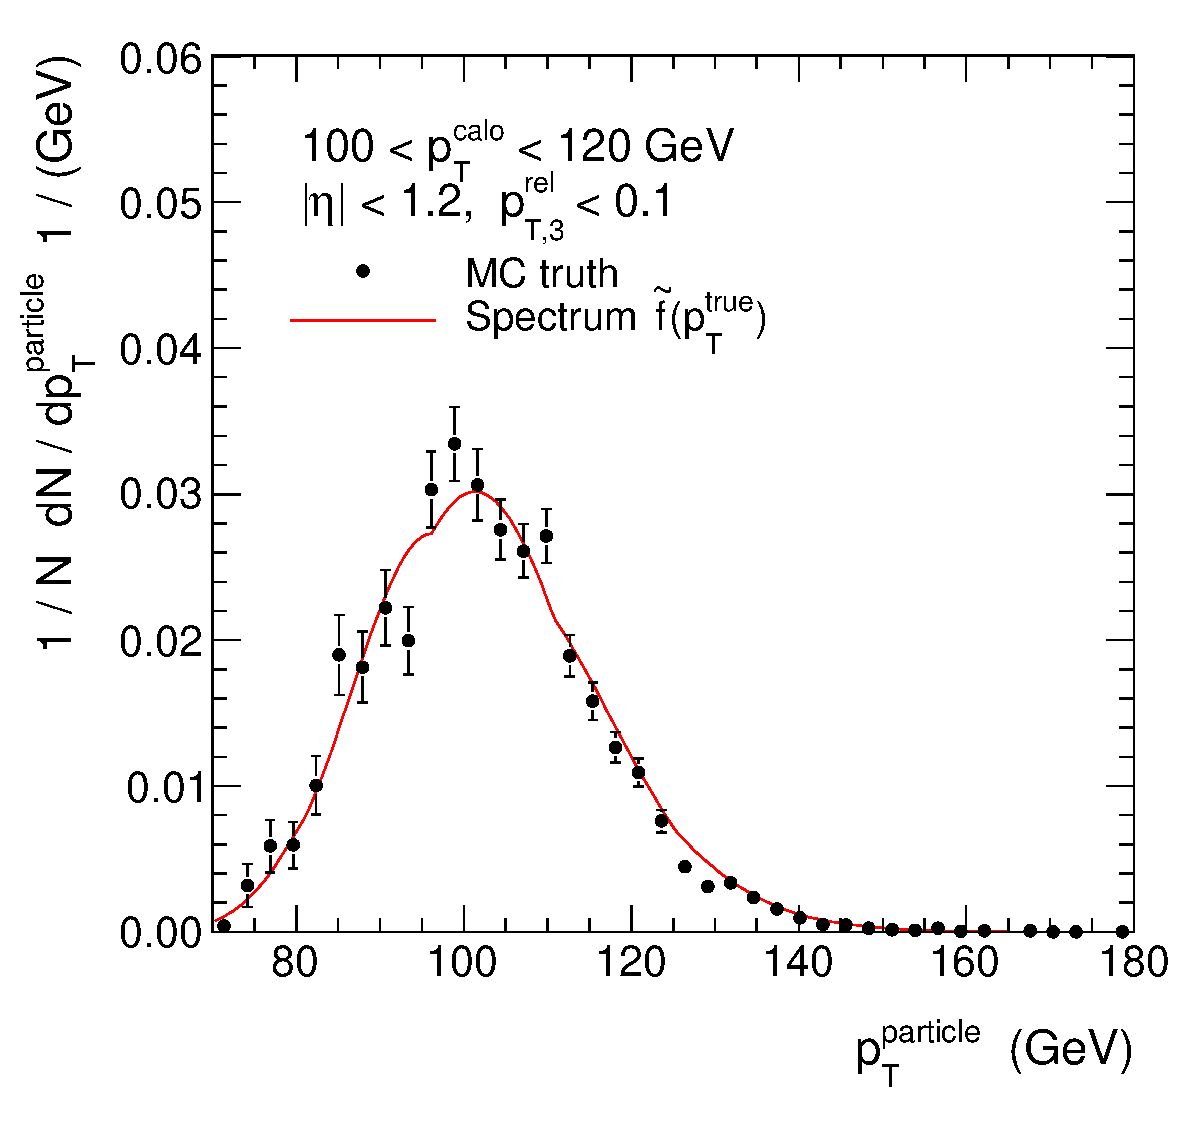
\includegraphics[width=0.3\textwidth]{figures/ResFit_Spring10QCDFlat_Gauss_Eta0_Spectrum_PtBin1} &
    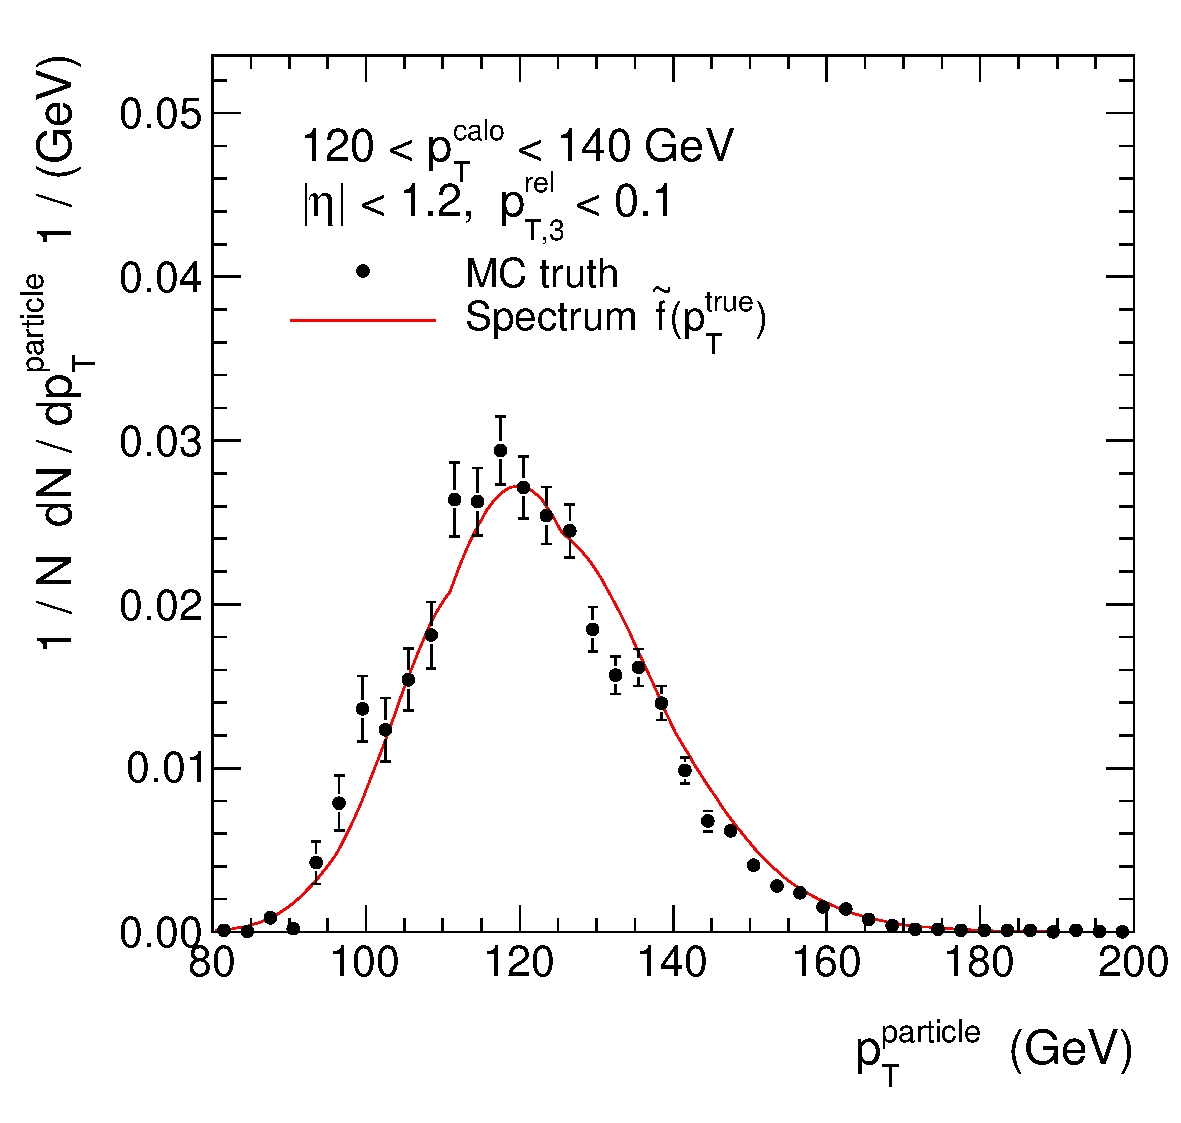
\includegraphics[width=0.3\textwidth]{figures/ResFit_Spring10QCDFlat_Gauss_Eta0_Spectrum_PtBin2} &
    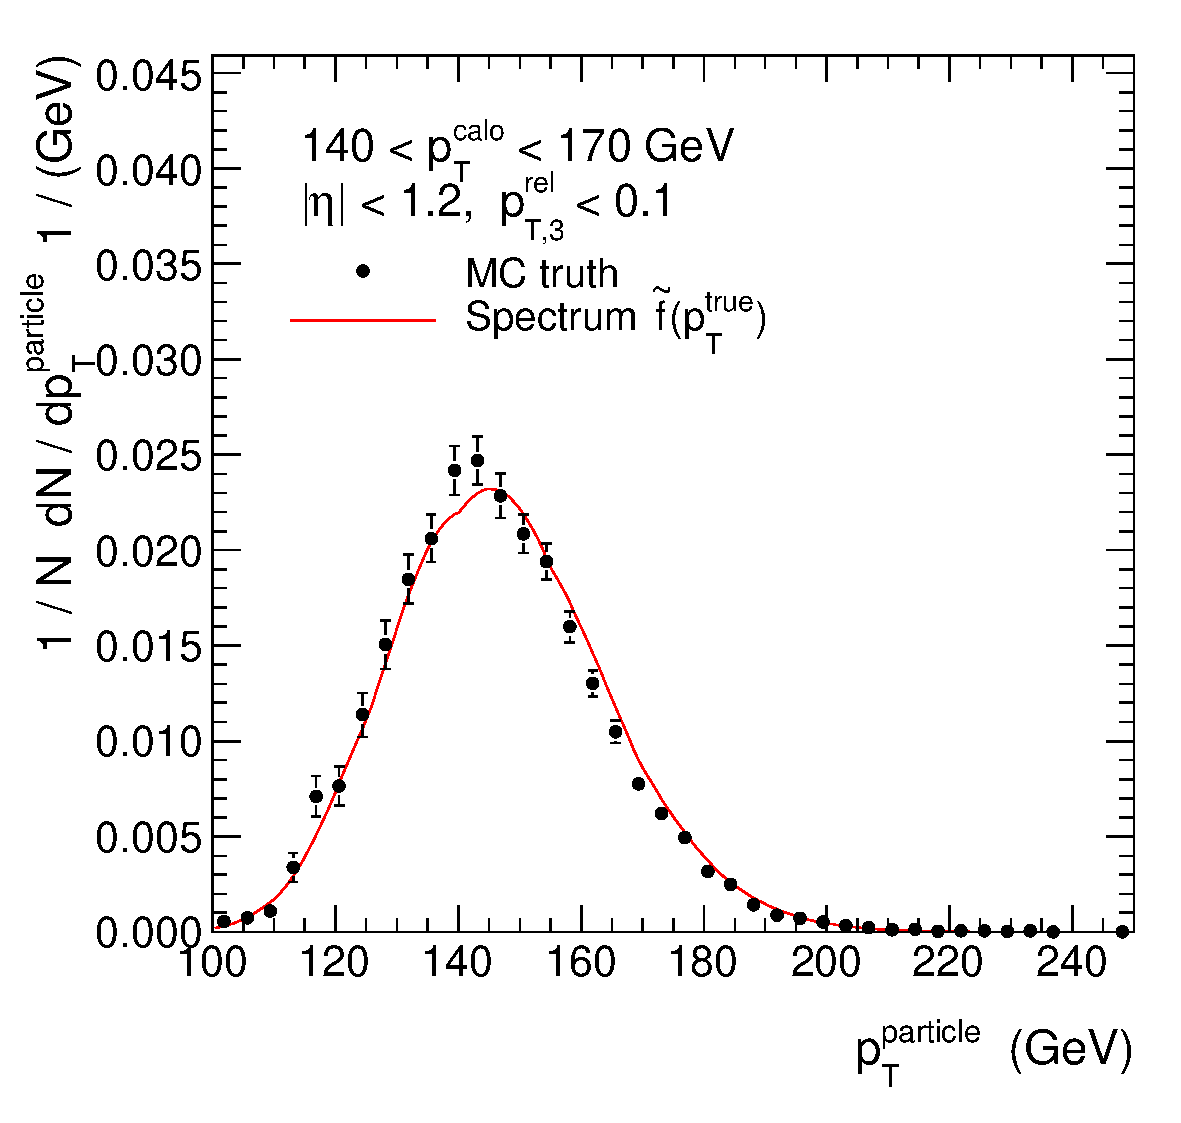
\includegraphics[width=0.3\textwidth]{figures/ResFit_Spring10QCDFlat_Gauss_Eta0_Spectrum_PtBin3} \\

    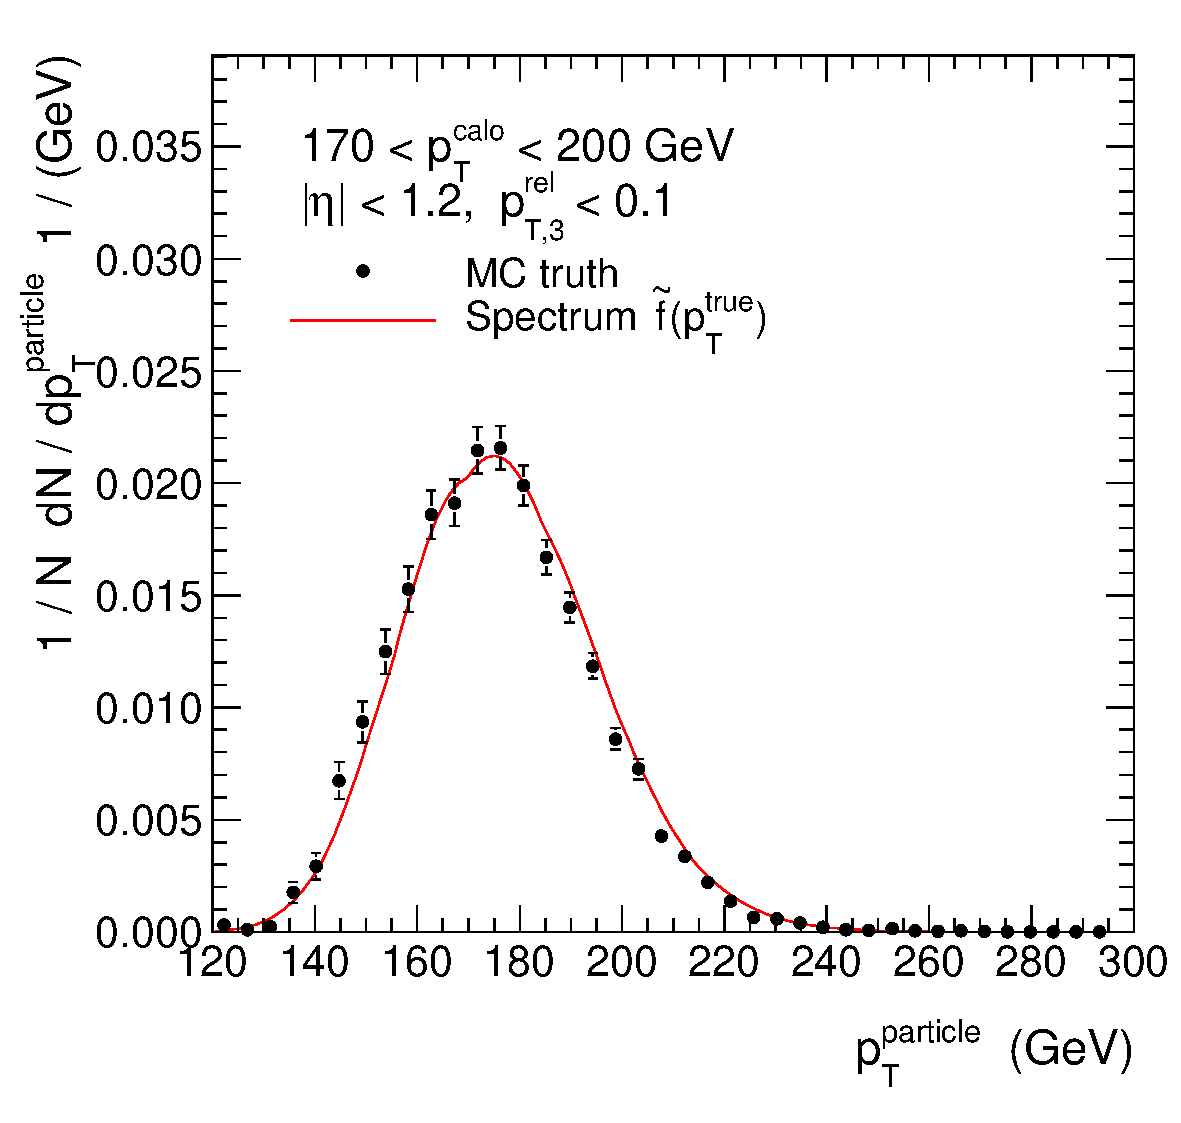
\includegraphics[width=0.3\textwidth]{figures/ResFit_Spring10QCDFlat_Gauss_Eta0_Spectrum_PtBin4} &
    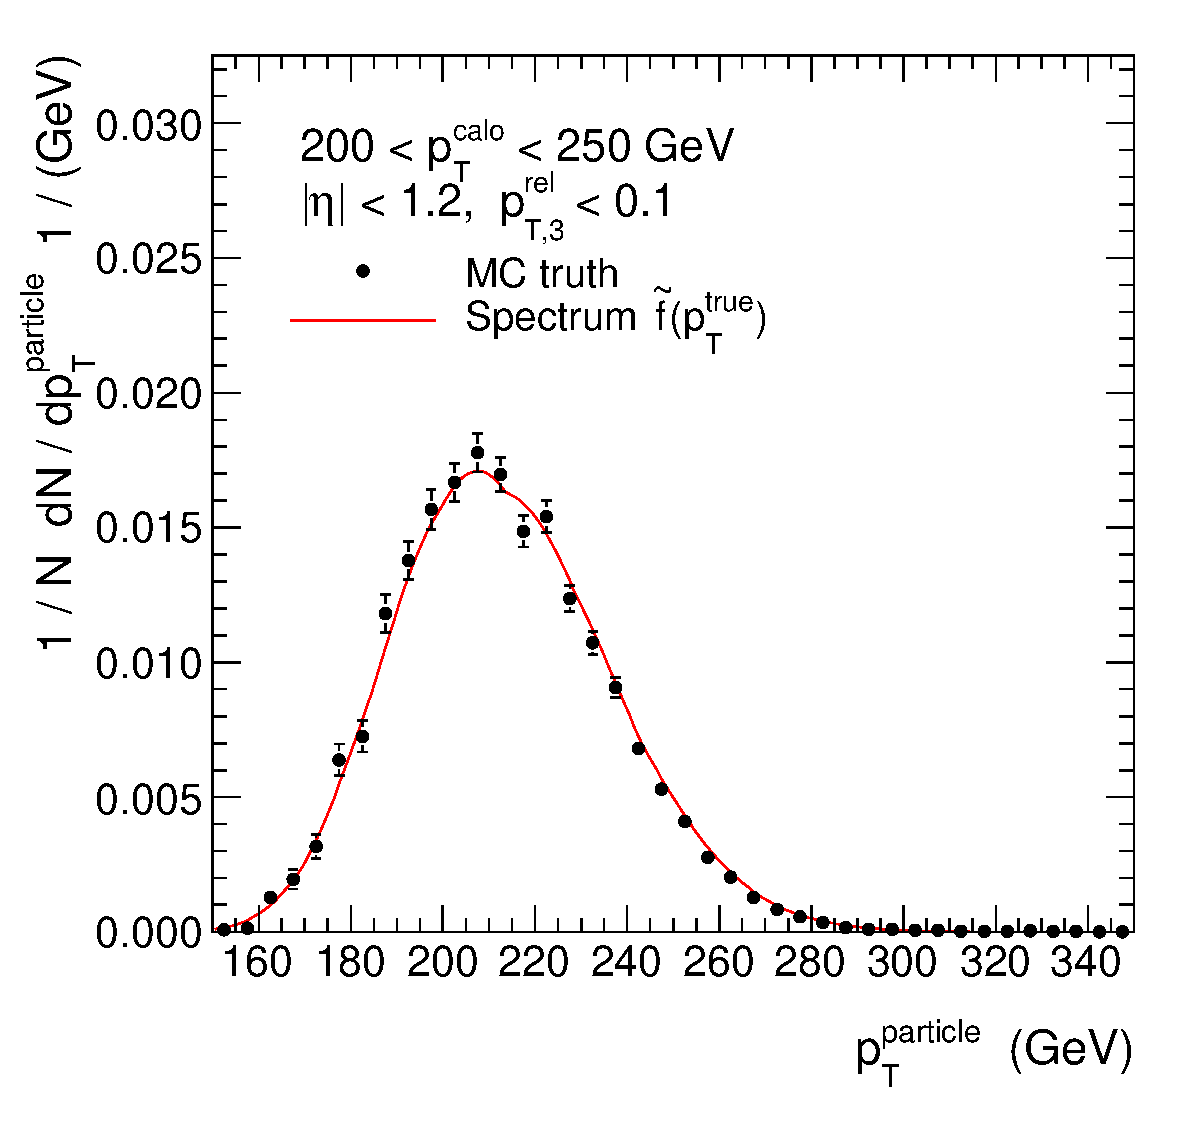
\includegraphics[width=0.3\textwidth]{figures/ResFit_Spring10QCDFlat_Gauss_Eta0_Spectrum_PtBin5} &
    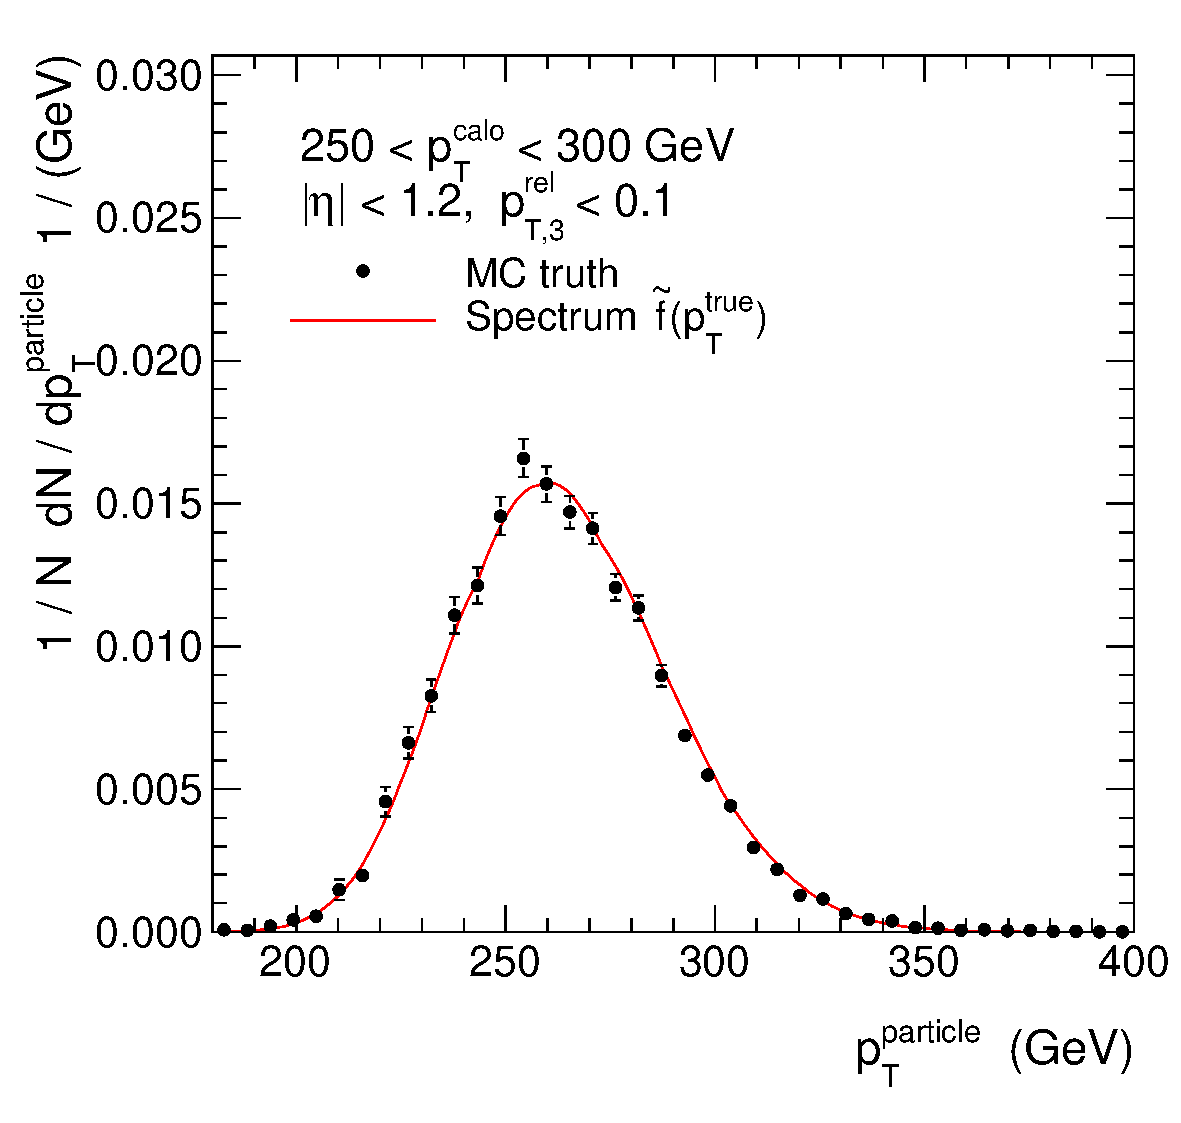
\includegraphics[width=0.3\textwidth]{figures/ResFit_Spring10QCDFlat_Gauss_Eta0_Spectrum_PtBin6} \\

    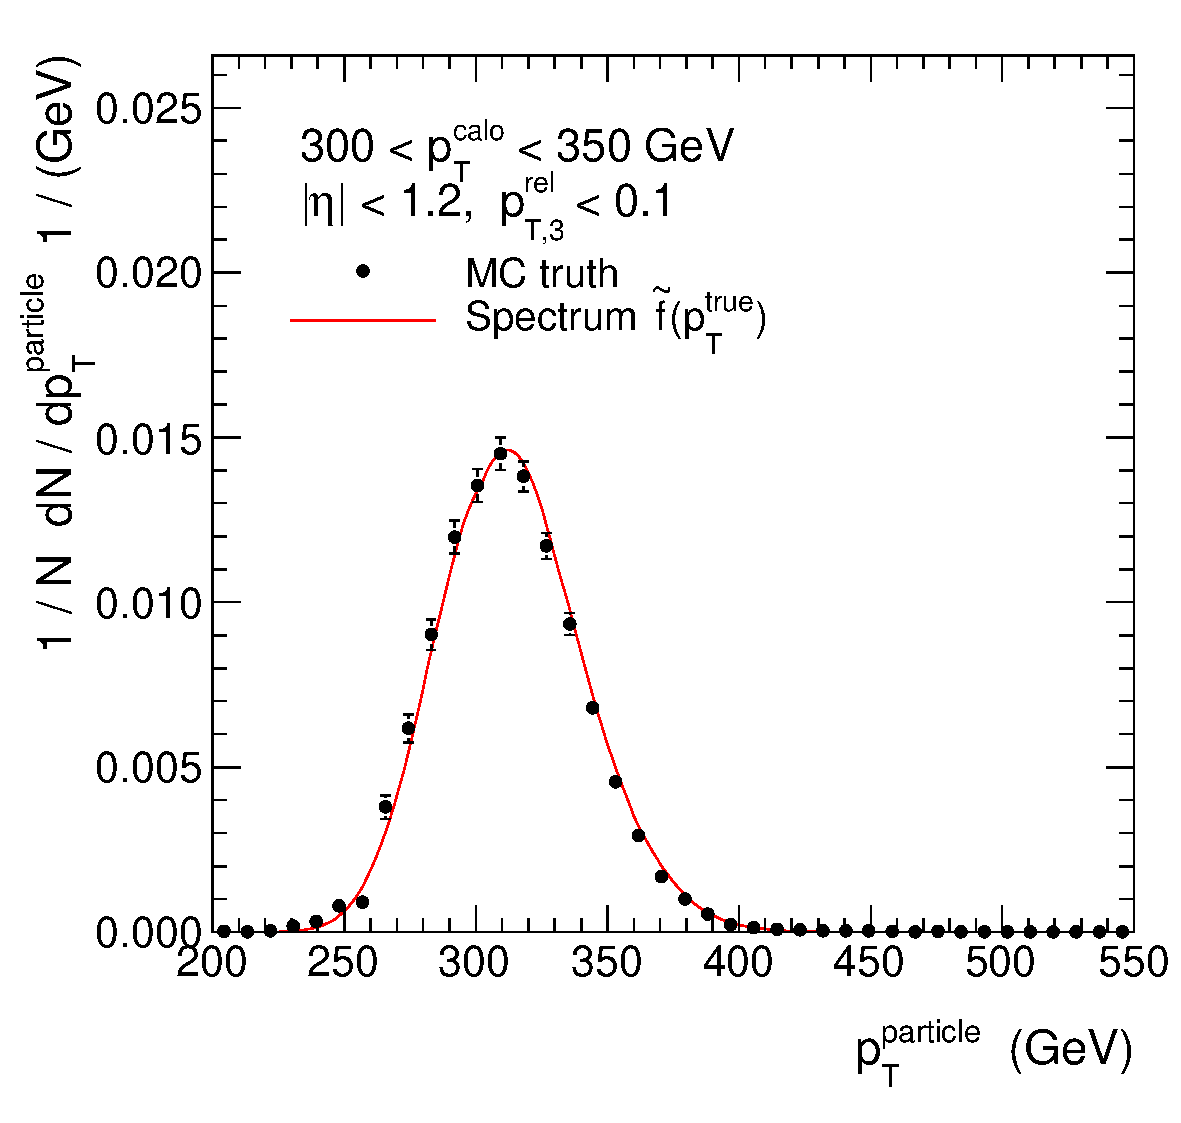
\includegraphics[width=0.3\textwidth]{figures/ResFit_Spring10QCDFlat_Gauss_Eta0_Spectrum_PtBin7} &
    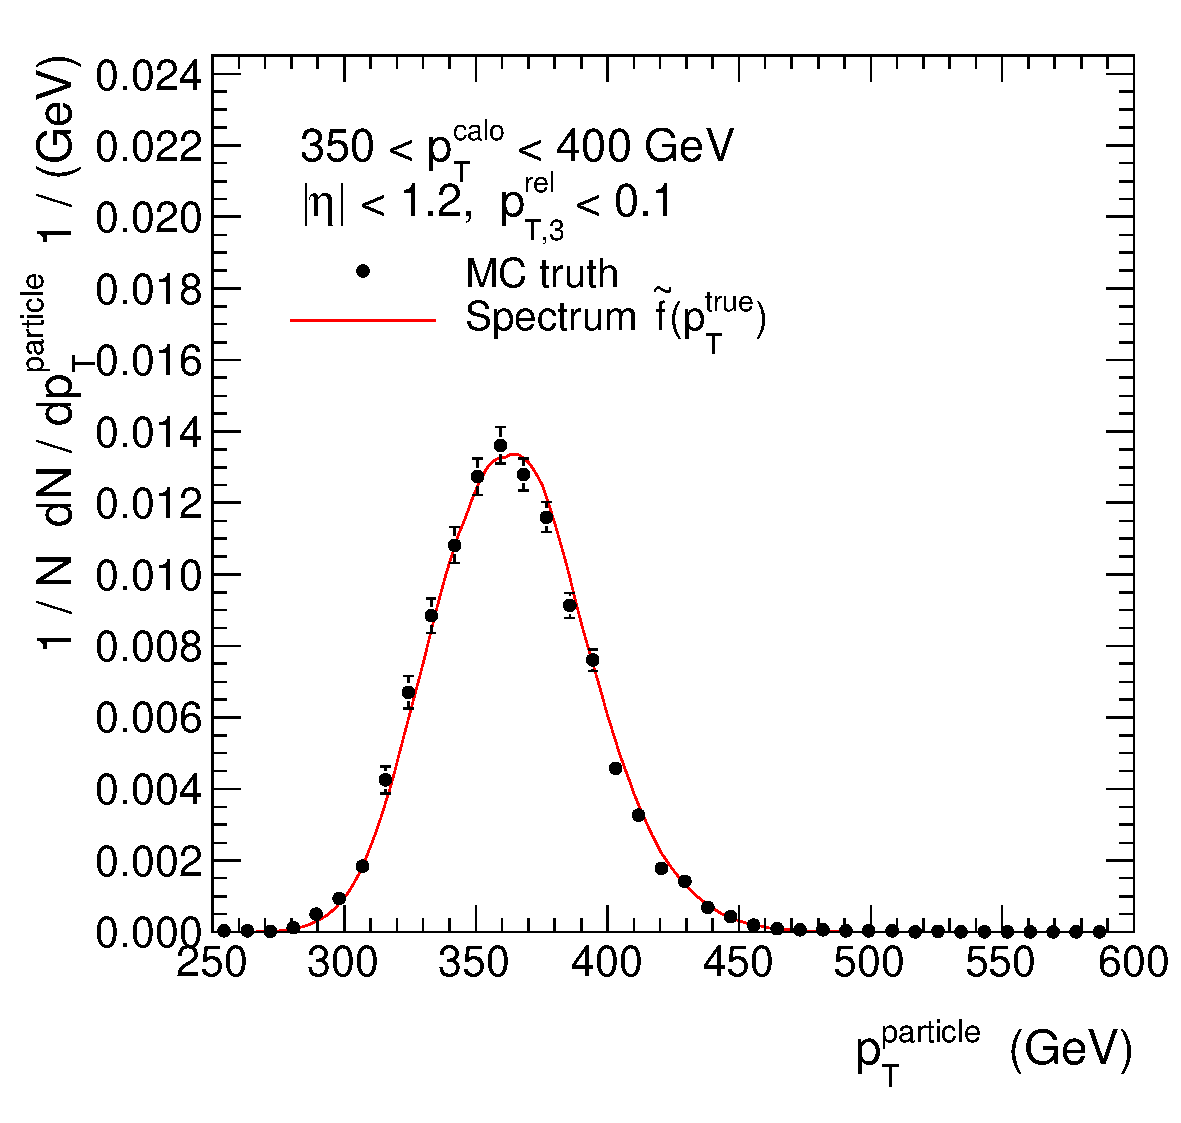
\includegraphics[width=0.3\textwidth]{figures/ResFit_Spring10QCDFlat_Gauss_Eta0_Spectrum_PtBin8} &
    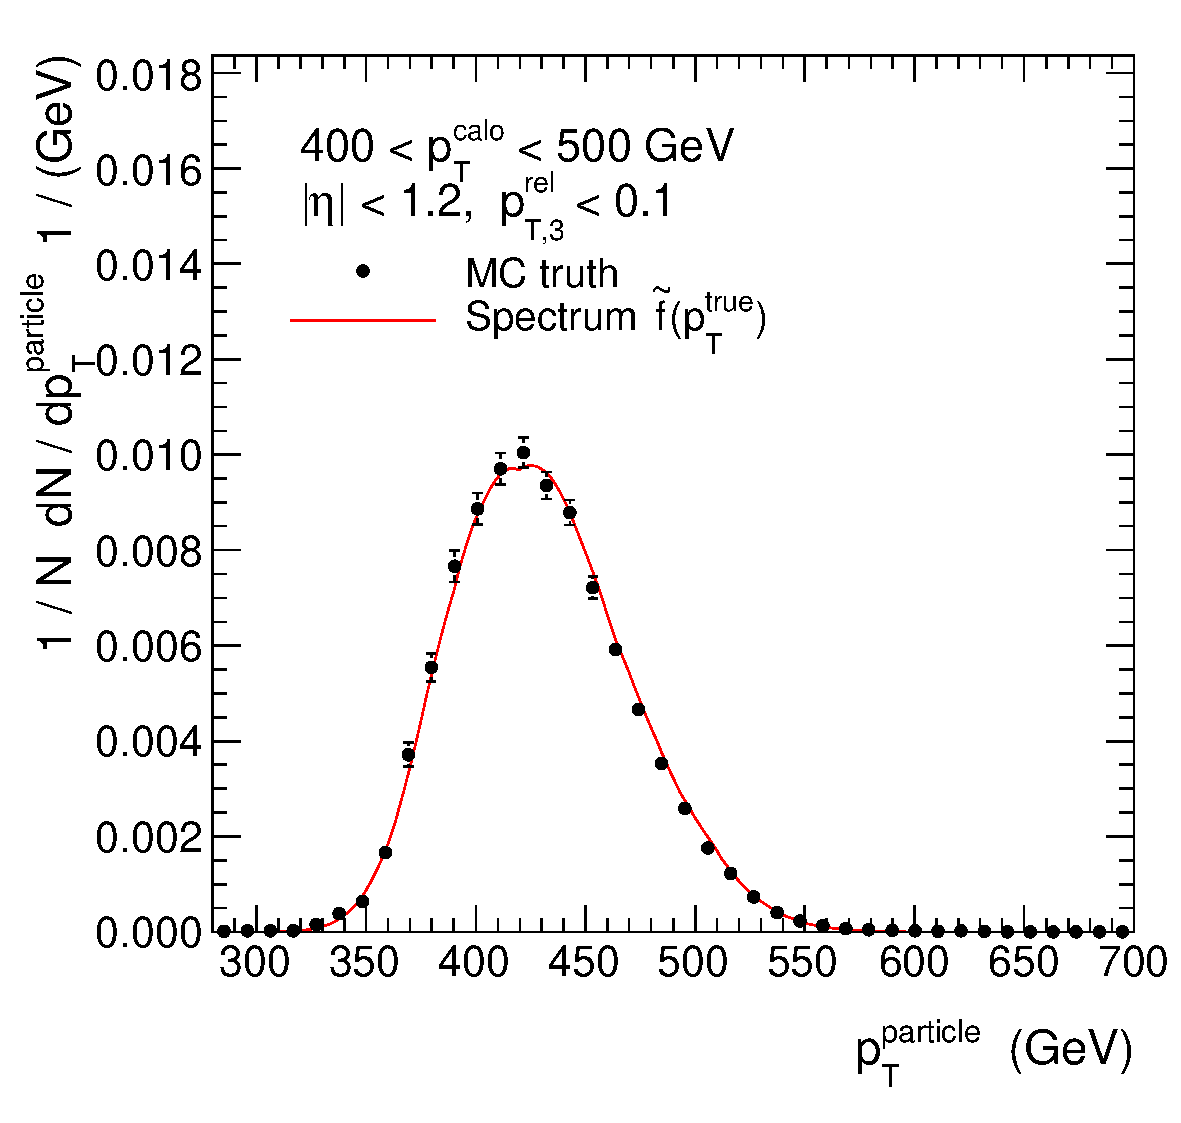
\includegraphics[width=0.3\textwidth]{figures/ResFit_Spring10QCDFlat_Gauss_Eta0_Spectrum_PtBin9} \\

    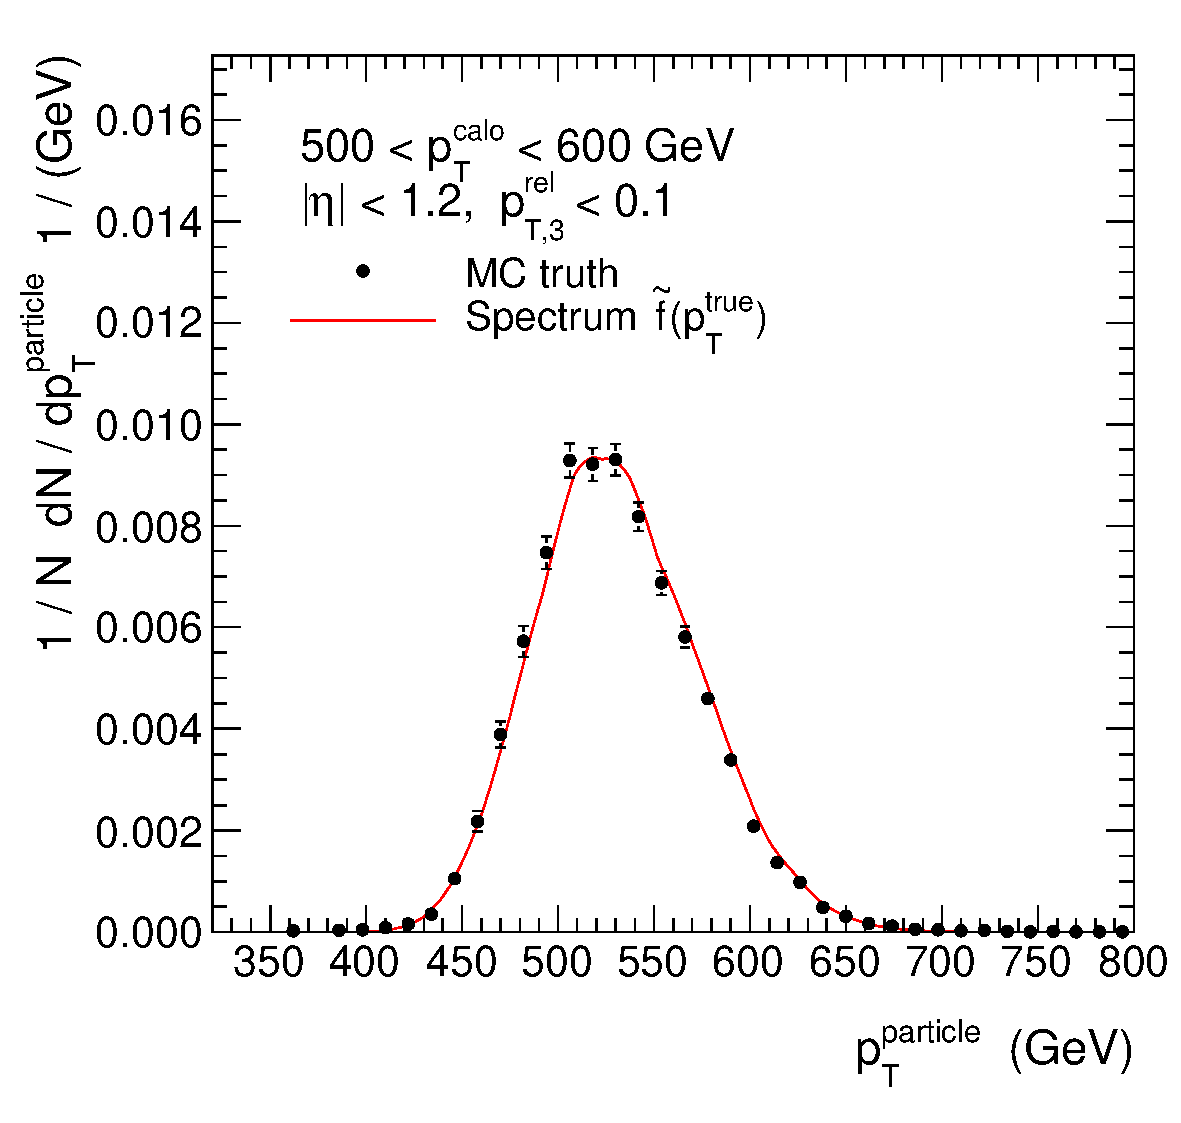
\includegraphics[width=0.3\textwidth]{figures/ResFit_Spring10QCDFlat_Gauss_Eta0_Spectrum_PtBin10} &
    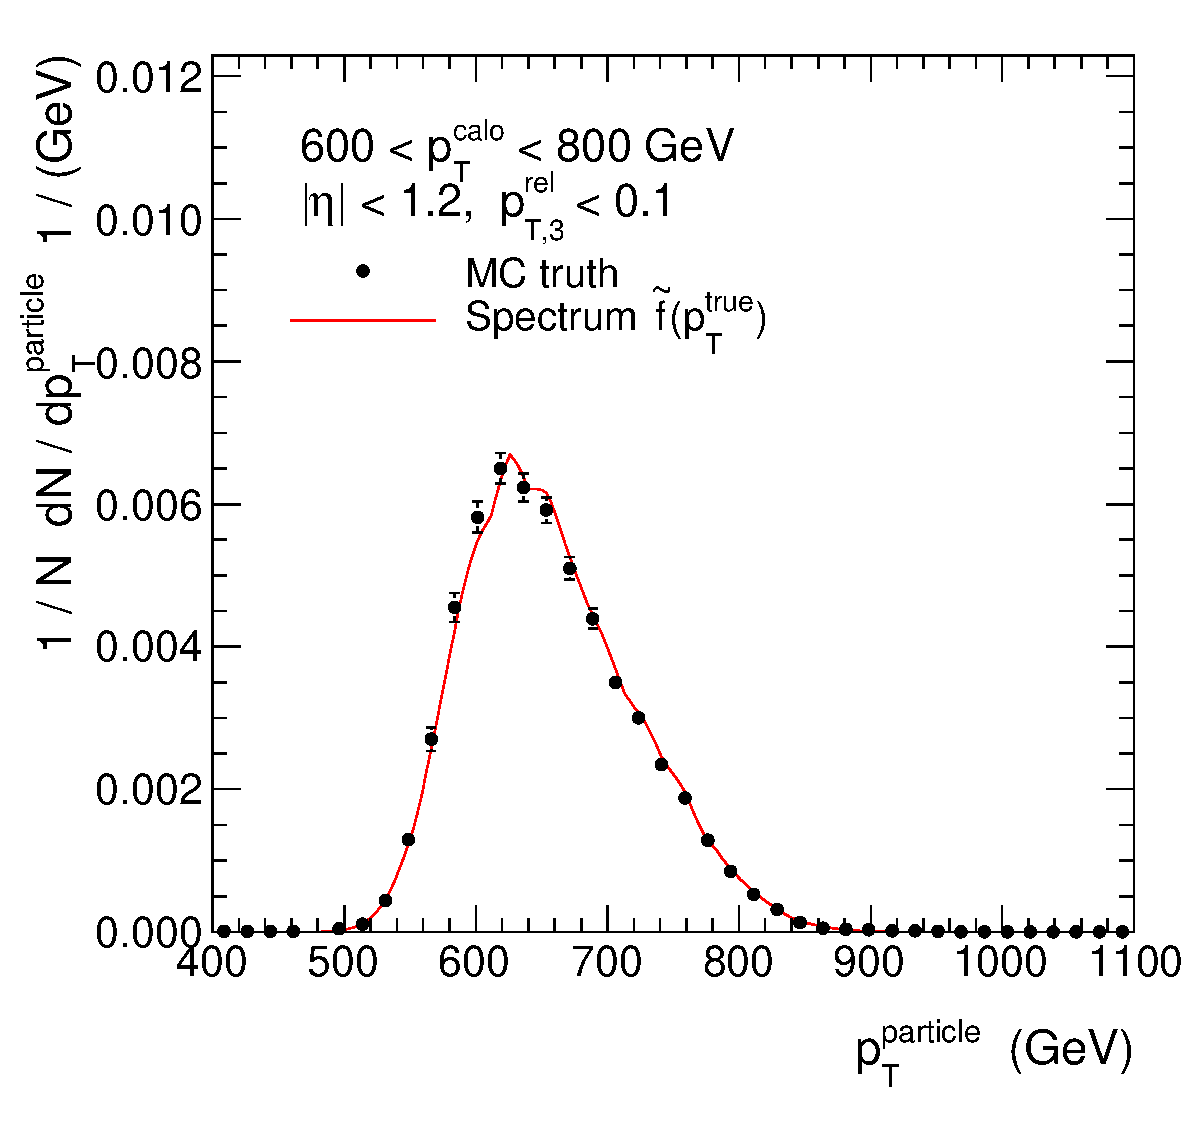
\includegraphics[width=0.3\textwidth]{figures/ResFit_Spring10QCDFlat_Gauss_Eta0_Spectrum_PtBin11} &
    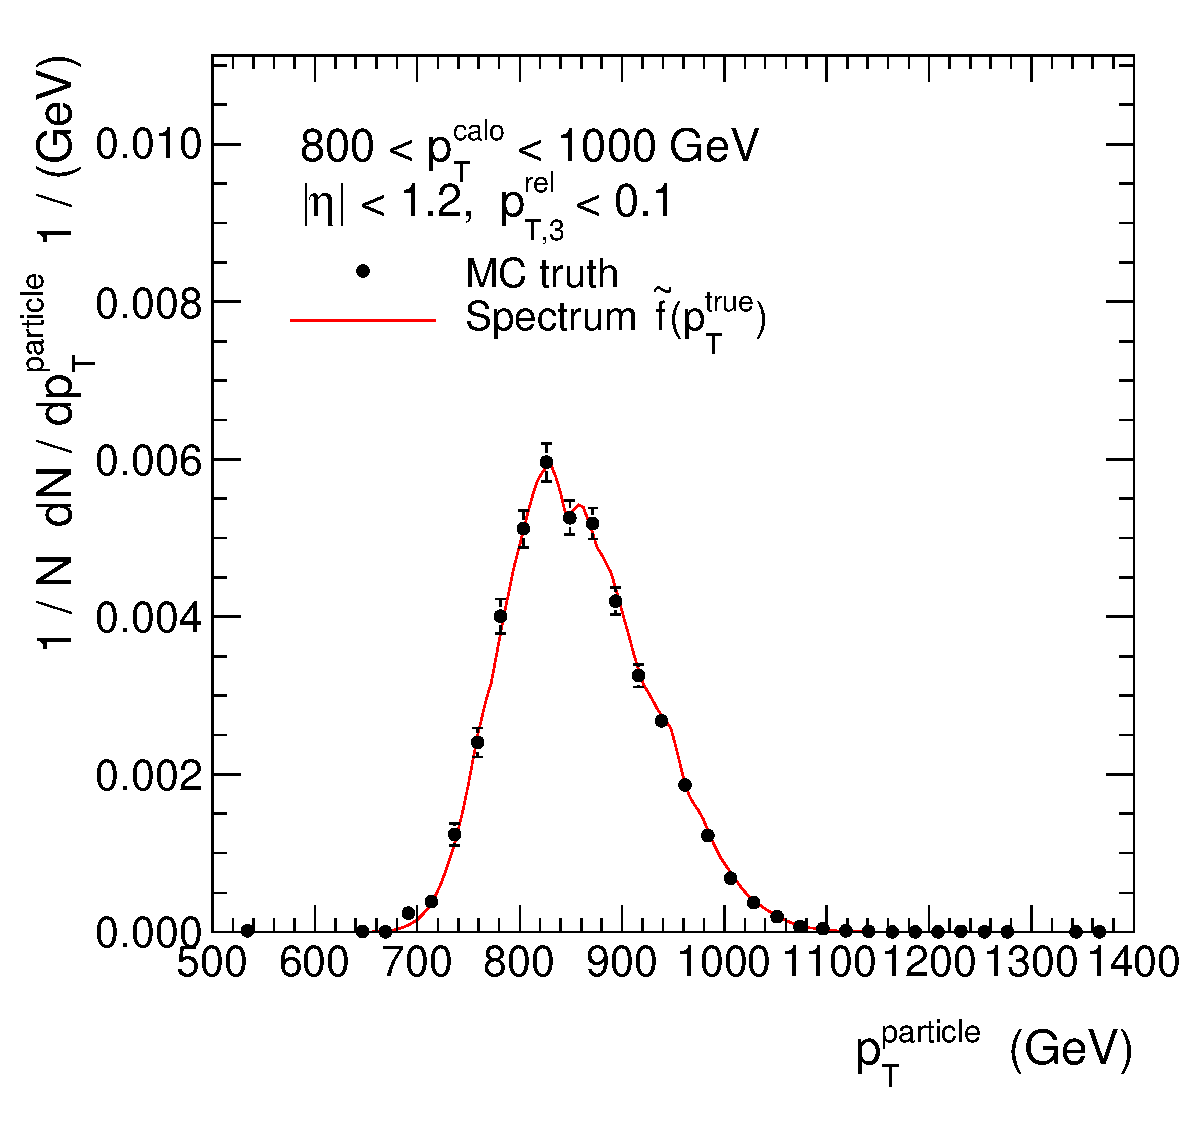
\includegraphics[width=0.3\textwidth]{figures/ResFit_Spring10QCDFlat_Gauss_Eta0_Spectrum_PtBin12} \\
  \end{tabular}
\caption{The parameterisation of the realistic particle jet \pt spectrum as used in the dijet likelihood (solid line) in comparison to the prediction from Monte Carlo truth (full circles) in different \pt bins for \mbox{$|\eta|<1.2$}. Migration effects are modeled assuming a Gaussian response function.}
\label{fig:ResFit:App:Gauss:Spectrum}
\end{figure}


% ----- Gauss Eta0 Extrapolations -----
\begin{figure}[ht]
  \centering
  \begin{tabular}{ccc}
    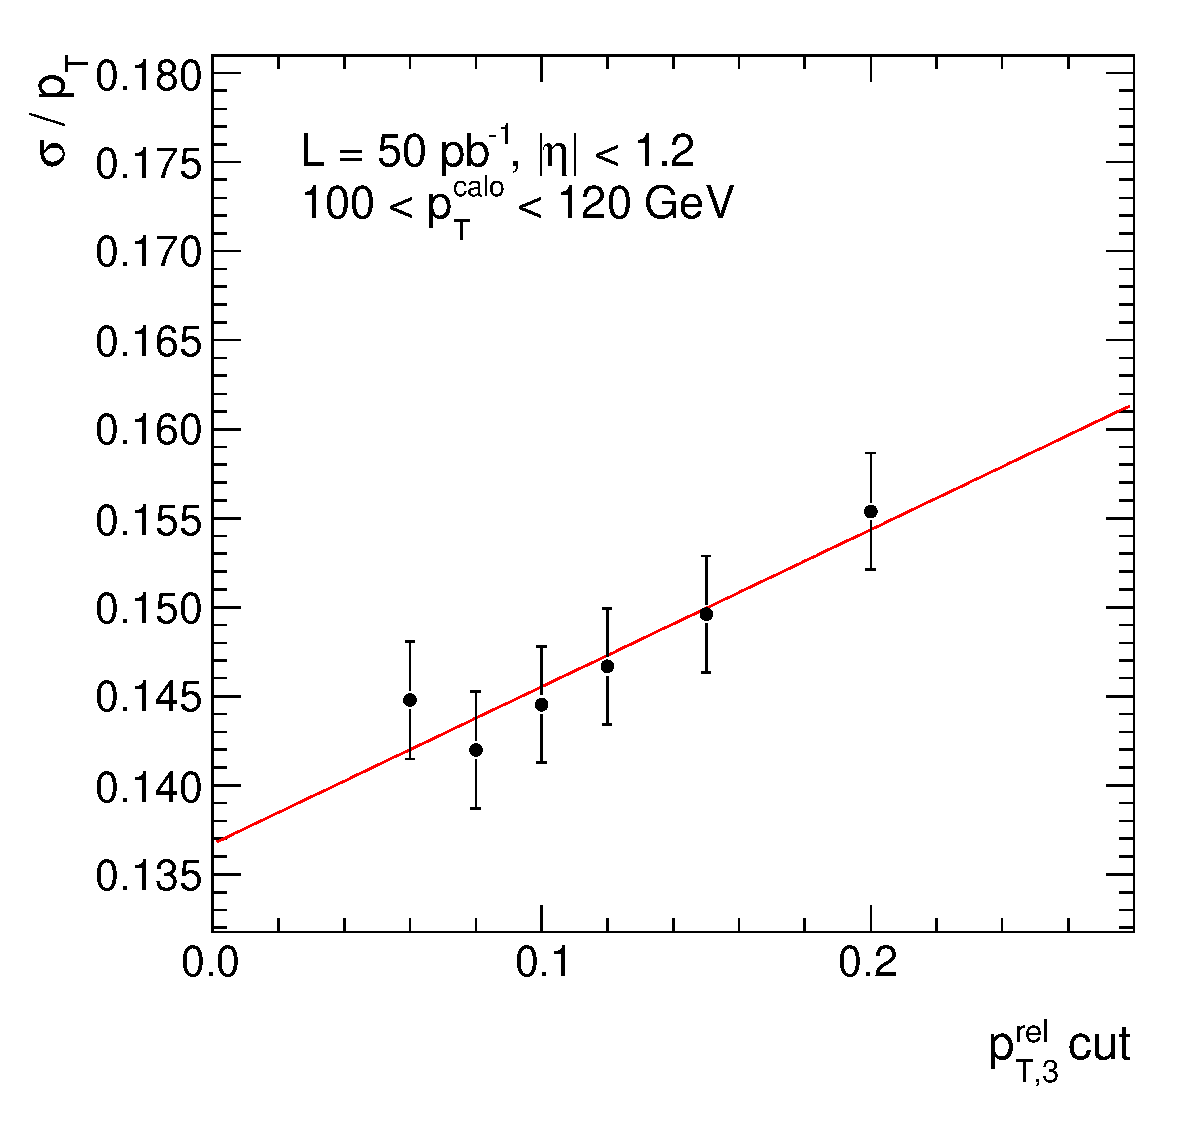
\includegraphics[width=0.3\textwidth]{figures/ResFit_Spring10QCDFlat_Gauss_Eta0_ExtrapolatedPar0_PtBin1} &
    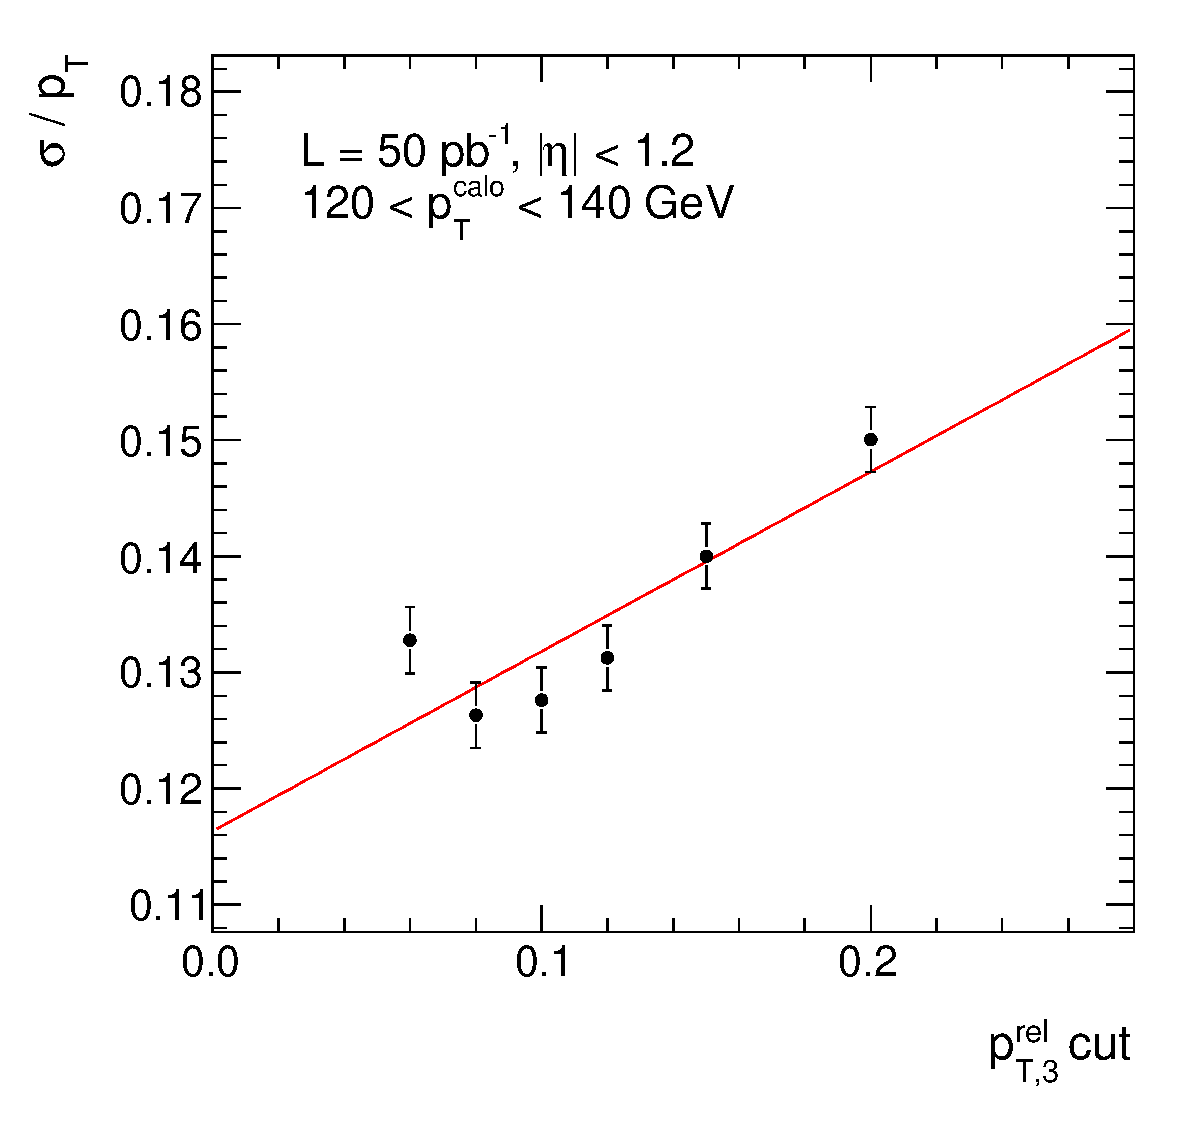
\includegraphics[width=0.3\textwidth]{figures/ResFit_Spring10QCDFlat_Gauss_Eta0_ExtrapolatedPar0_PtBin2} &
    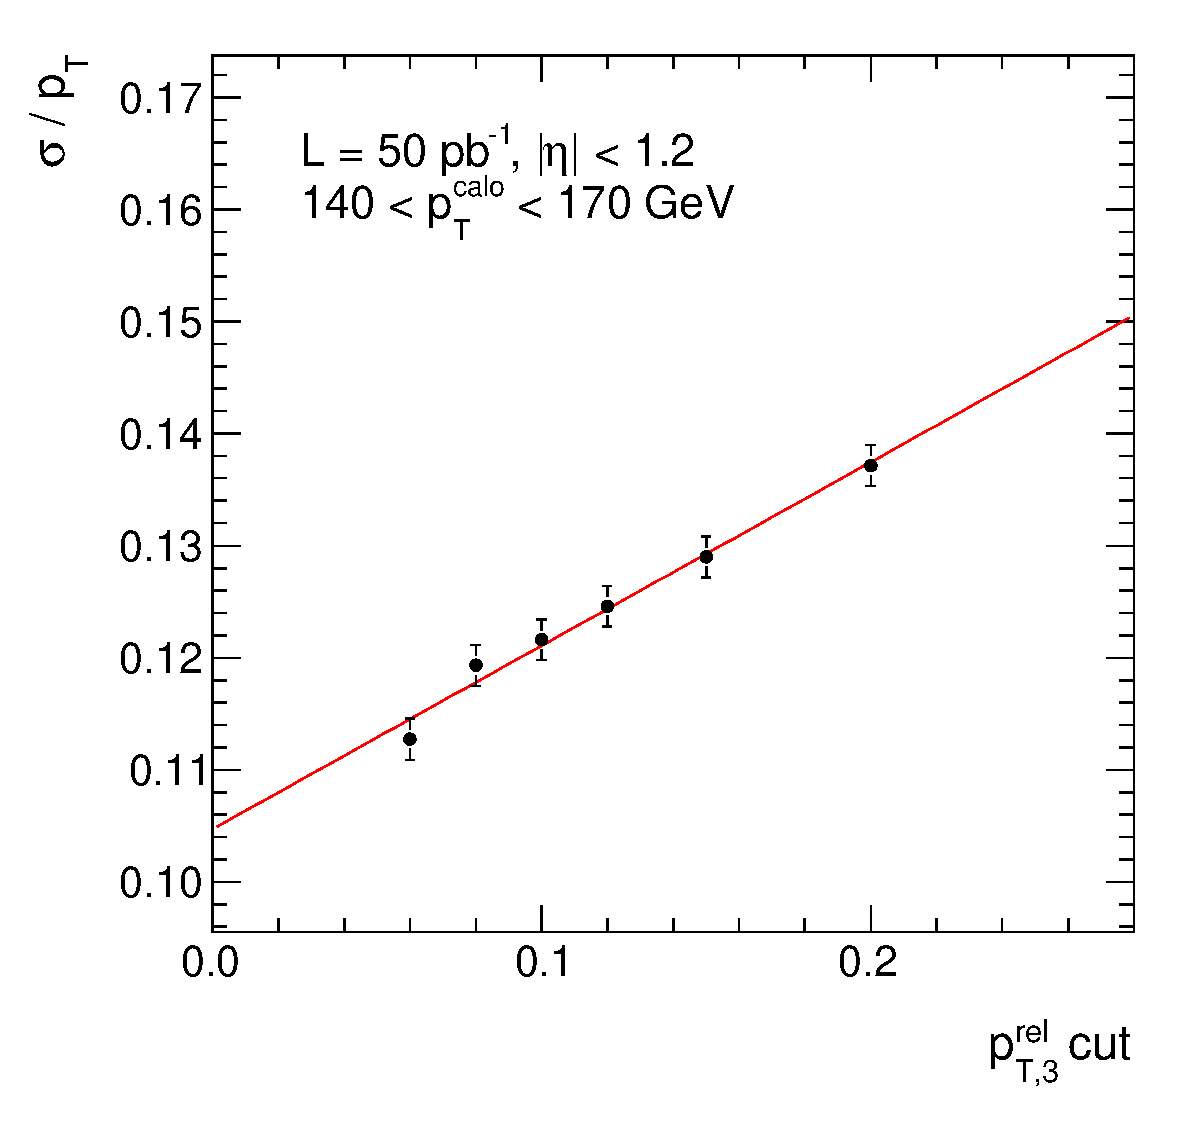
\includegraphics[width=0.3\textwidth]{figures/ResFit_Spring10QCDFlat_Gauss_Eta0_ExtrapolatedPar0_PtBin3} \\

    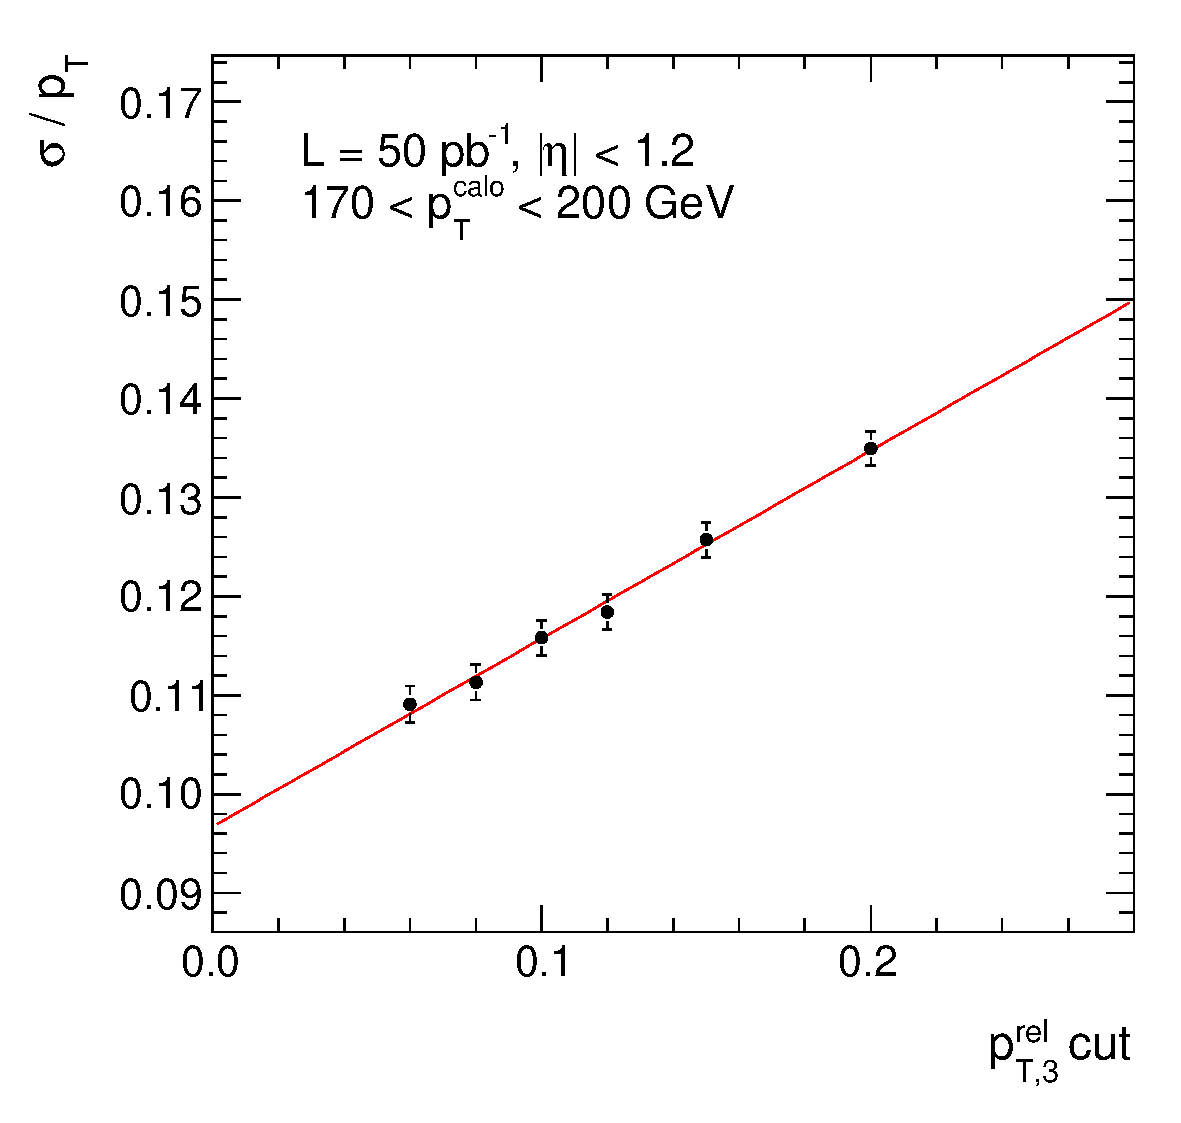
\includegraphics[width=0.3\textwidth]{figures/ResFit_Spring10QCDFlat_Gauss_Eta0_ExtrapolatedPar0_PtBin4} &
    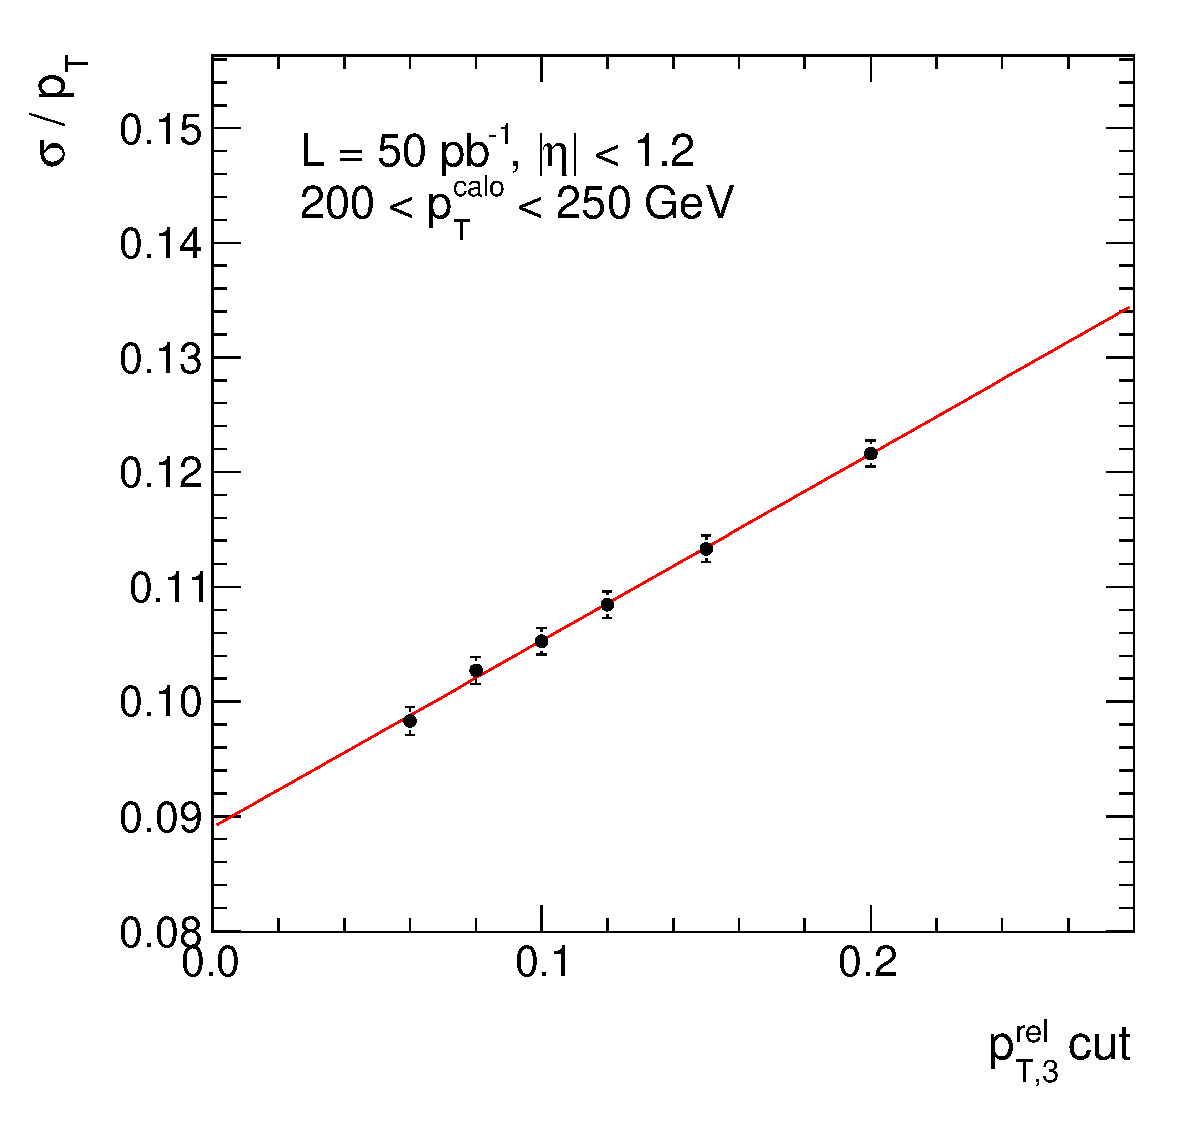
\includegraphics[width=0.3\textwidth]{figures/ResFit_Spring10QCDFlat_Gauss_Eta0_ExtrapolatedPar0_PtBin5} &
    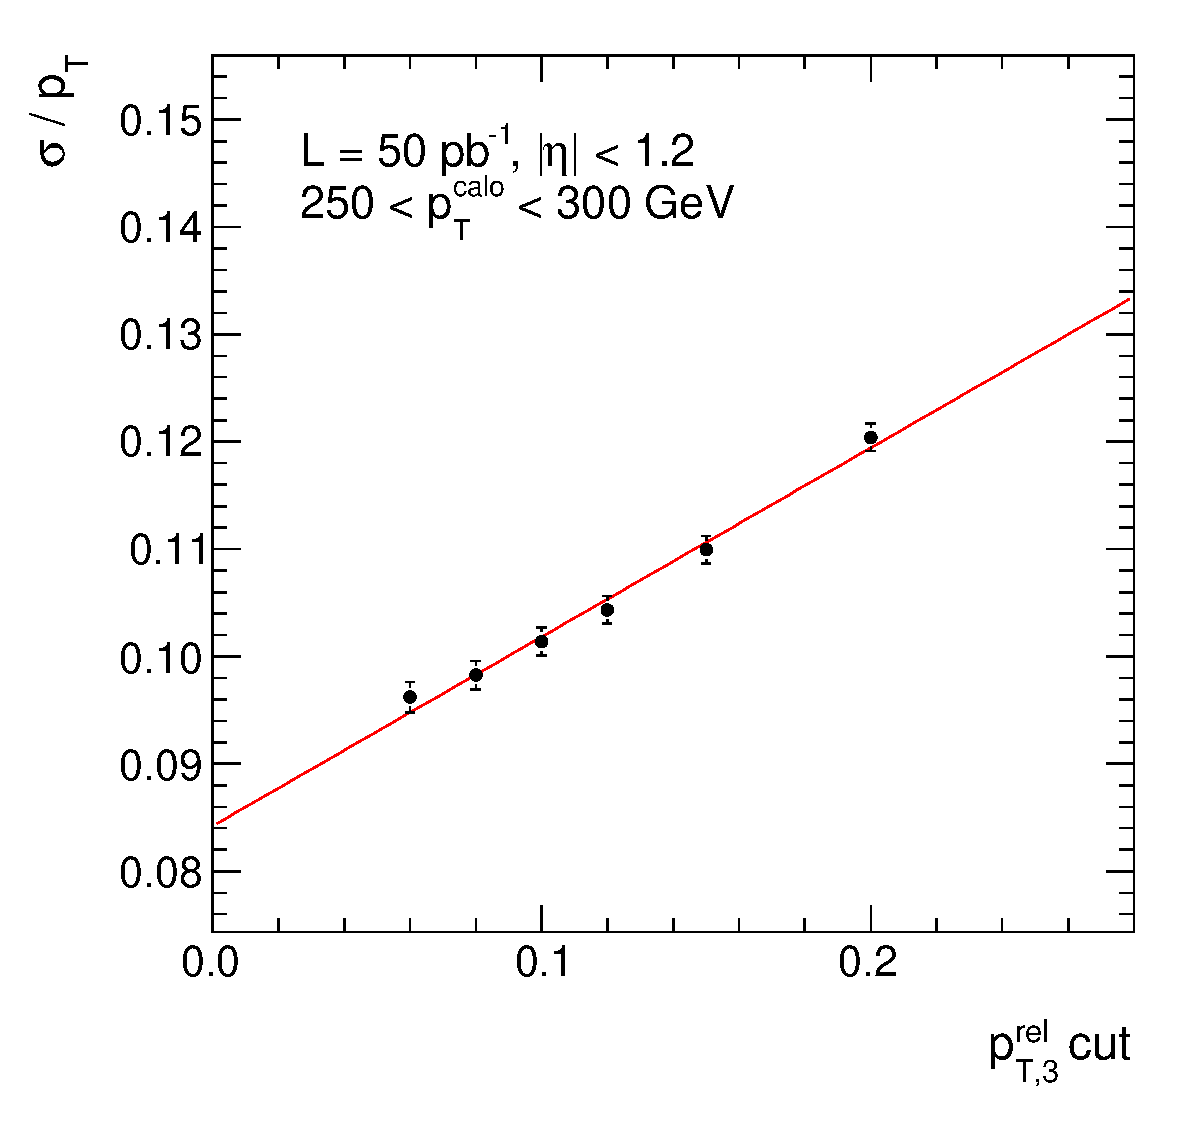
\includegraphics[width=0.3\textwidth]{figures/ResFit_Spring10QCDFlat_Gauss_Eta0_ExtrapolatedPar0_PtBin6} \\

    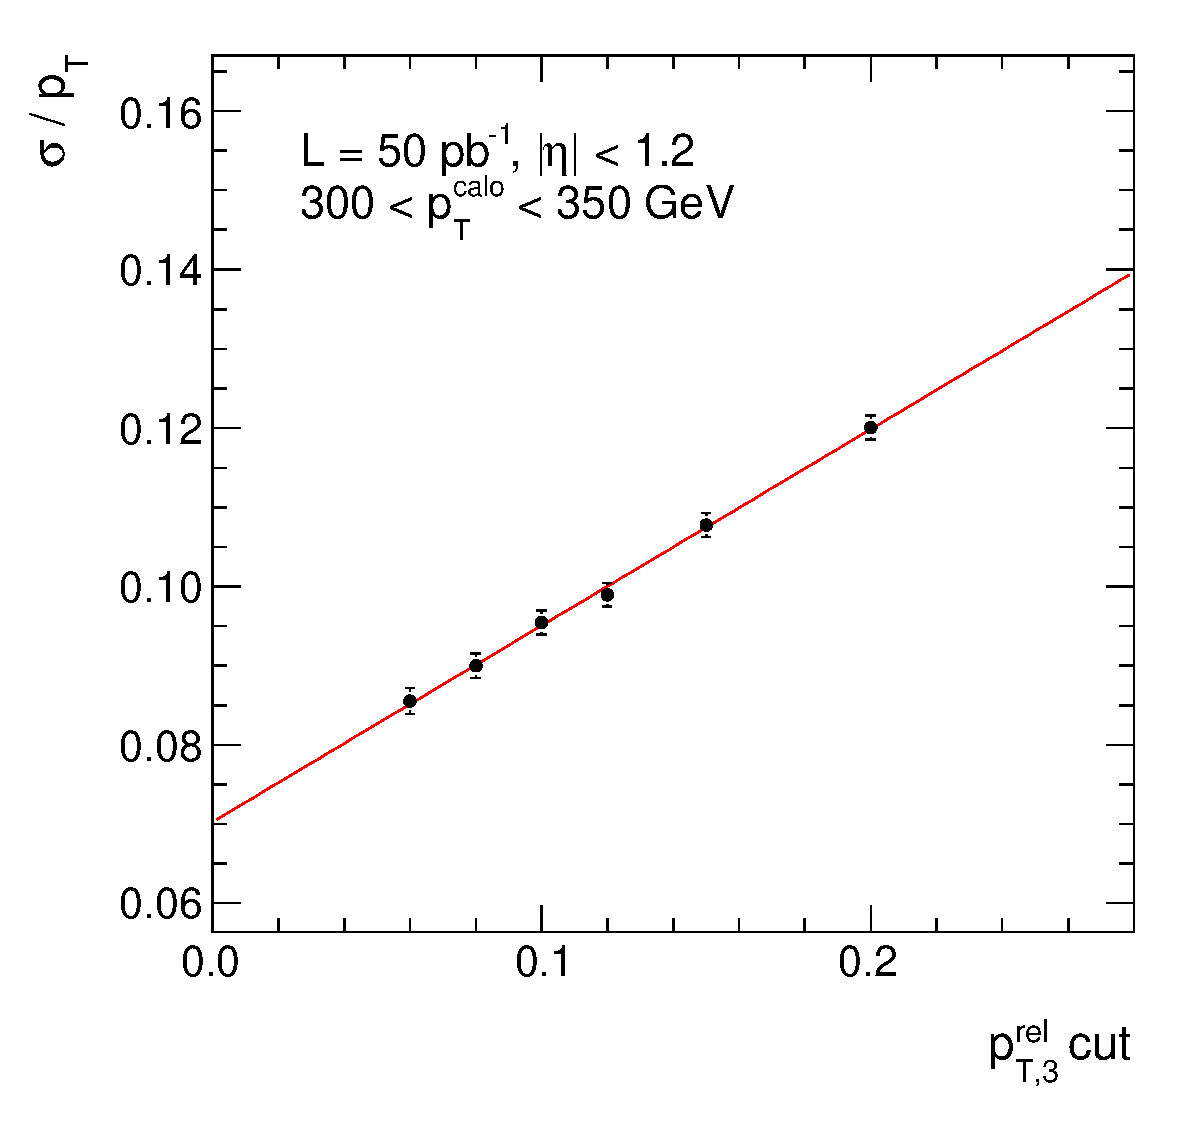
\includegraphics[width=0.3\textwidth]{figures/ResFit_Spring10QCDFlat_Gauss_Eta0_ExtrapolatedPar0_PtBin7} &
    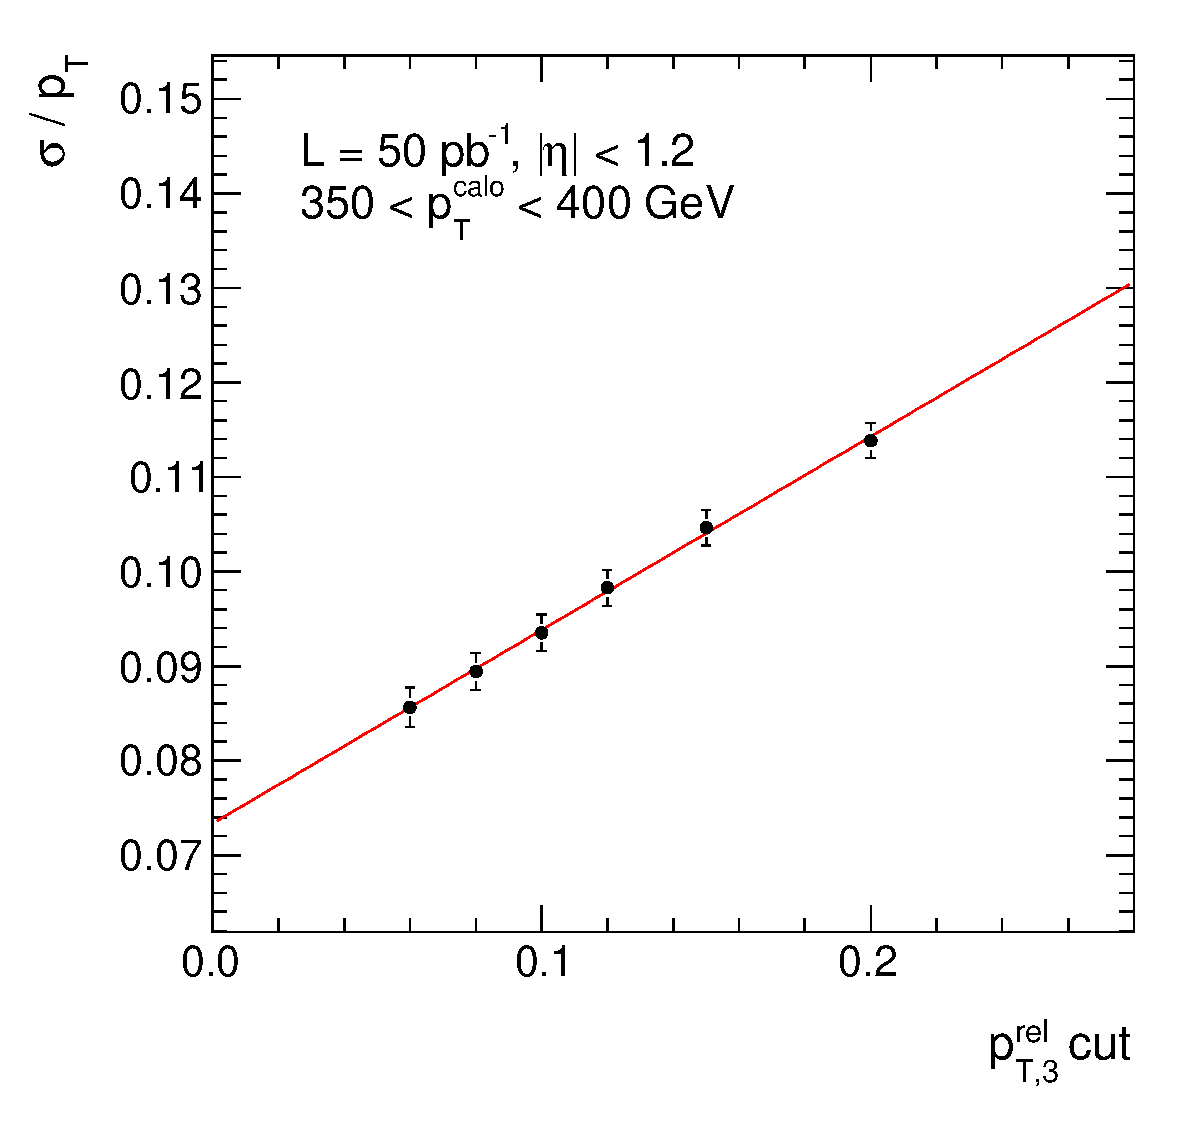
\includegraphics[width=0.3\textwidth]{figures/ResFit_Spring10QCDFlat_Gauss_Eta0_ExtrapolatedPar0_PtBin8} &
    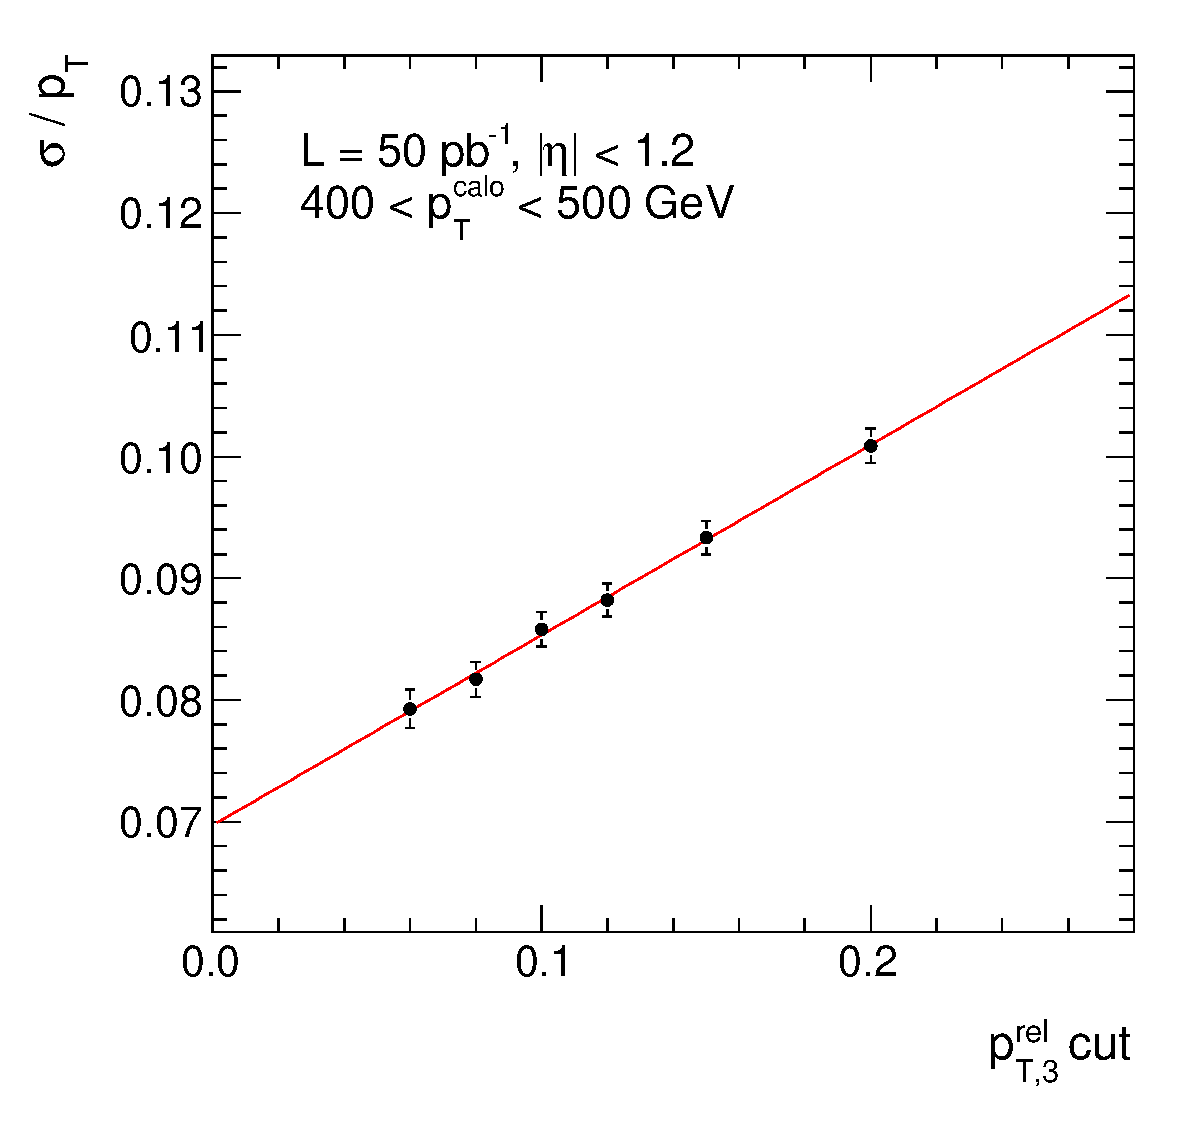
\includegraphics[width=0.3\textwidth]{figures/ResFit_Spring10QCDFlat_Gauss_Eta0_ExtrapolatedPar0_PtBin9} \\

    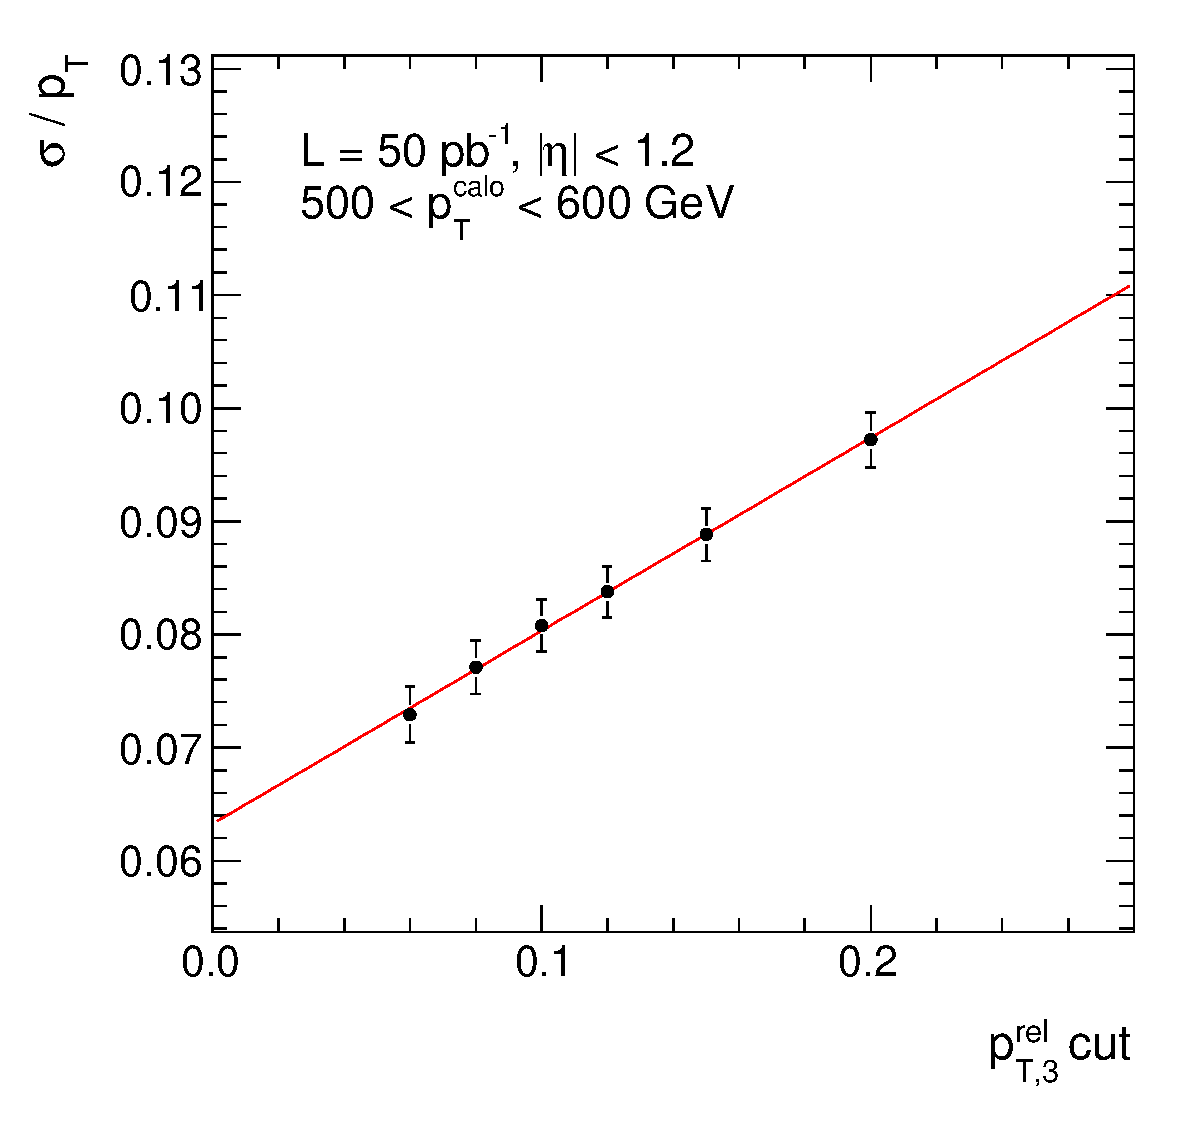
\includegraphics[width=0.3\textwidth]{figures/ResFit_Spring10QCDFlat_Gauss_Eta0_ExtrapolatedPar0_PtBin10} &
    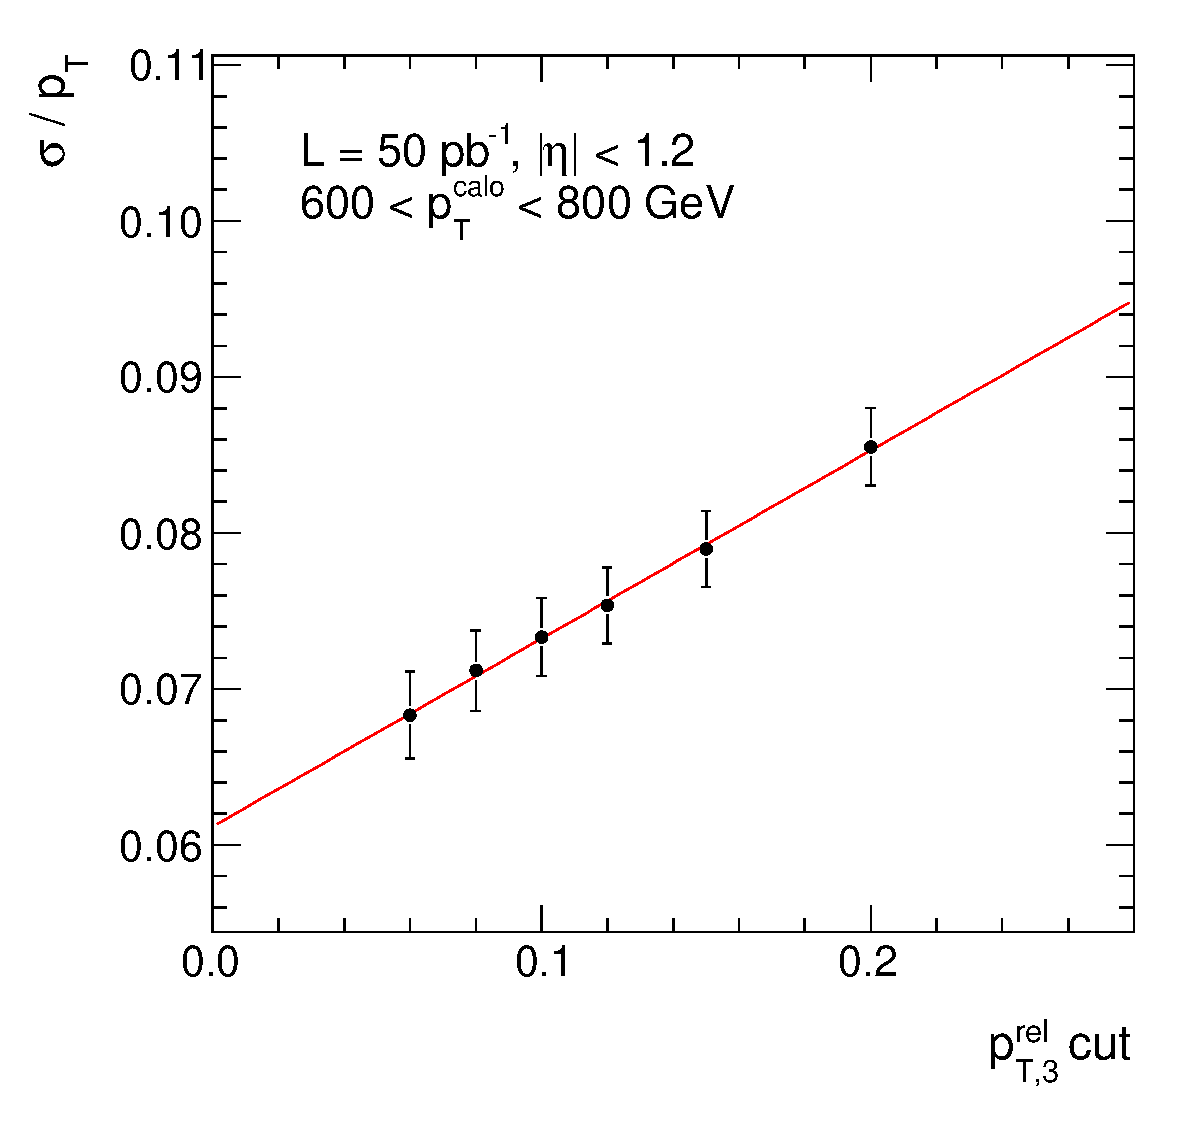
\includegraphics[width=0.3\textwidth]{figures/ResFit_Spring10QCDFlat_Gauss_Eta0_ExtrapolatedPar0_PtBin11} &
    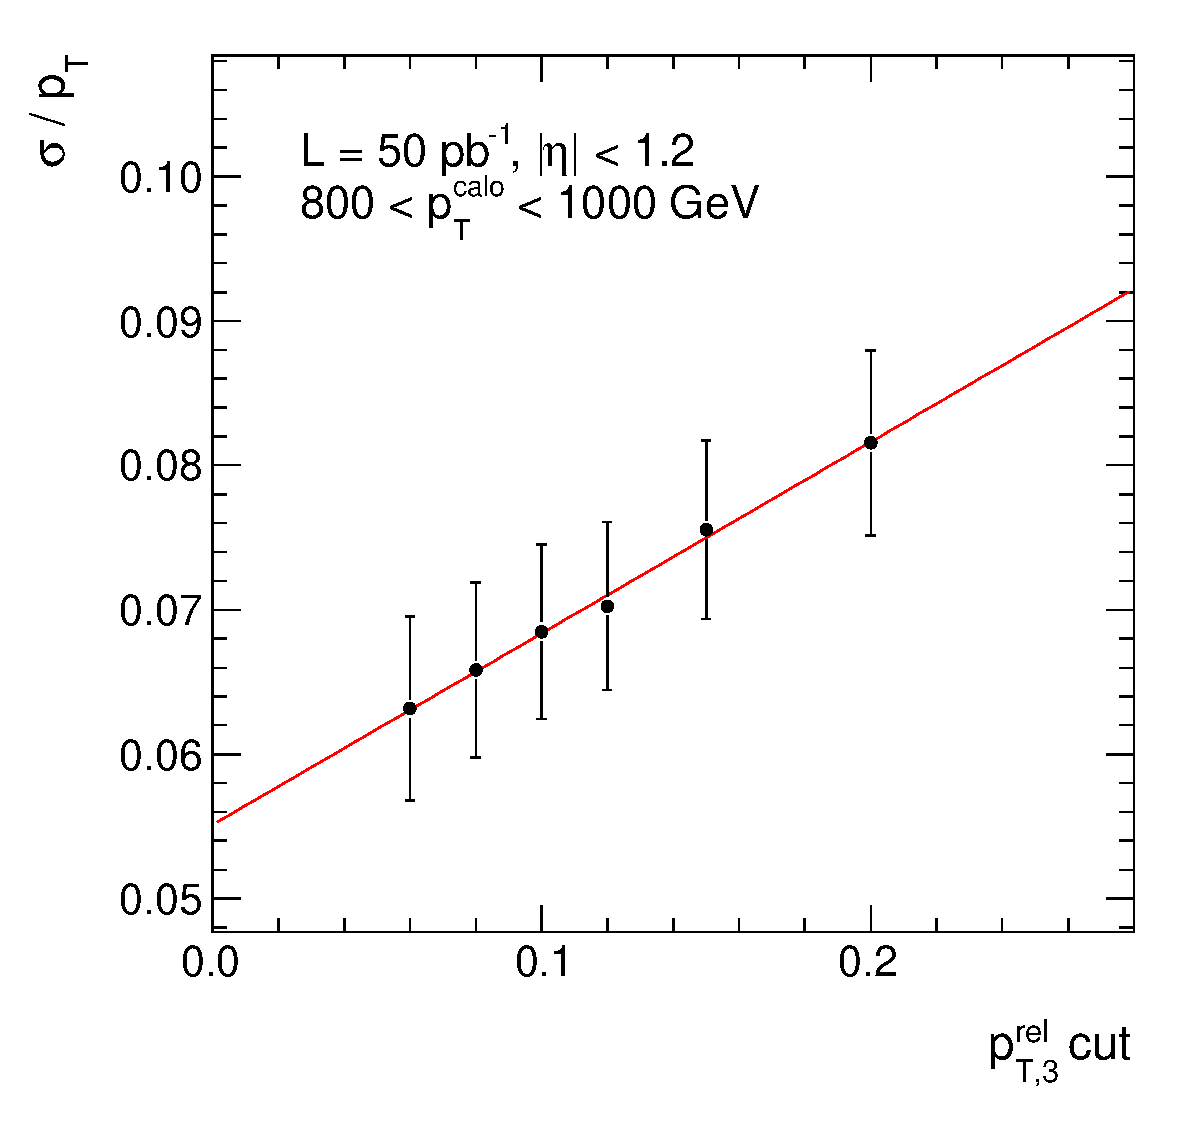
\includegraphics[width=0.3\textwidth]{figures/ResFit_Spring10QCDFlat_Gauss_Eta0_ExtrapolatedPar0_PtBin12} \\
  \end{tabular}
\caption{Resolutions $\bar{\sigma}/\pt$ from Gaussian fits for different limits on \ptrel in different \pt bins for \mbox{$|\eta|<1.2$}.
  The solid line is a linear fit to extrapolate $\bar{\sigma}/\pt$ to the ideal case of only two jets in the
  final state.}
\label{fig:ResFit:App:Gauss:Extrapolation}
\end{figure}


% ----- Gauss Eta0 MC truth closure -----
\begin{figure}[ht]
  \centering
  \begin{tabular}{ccc}
    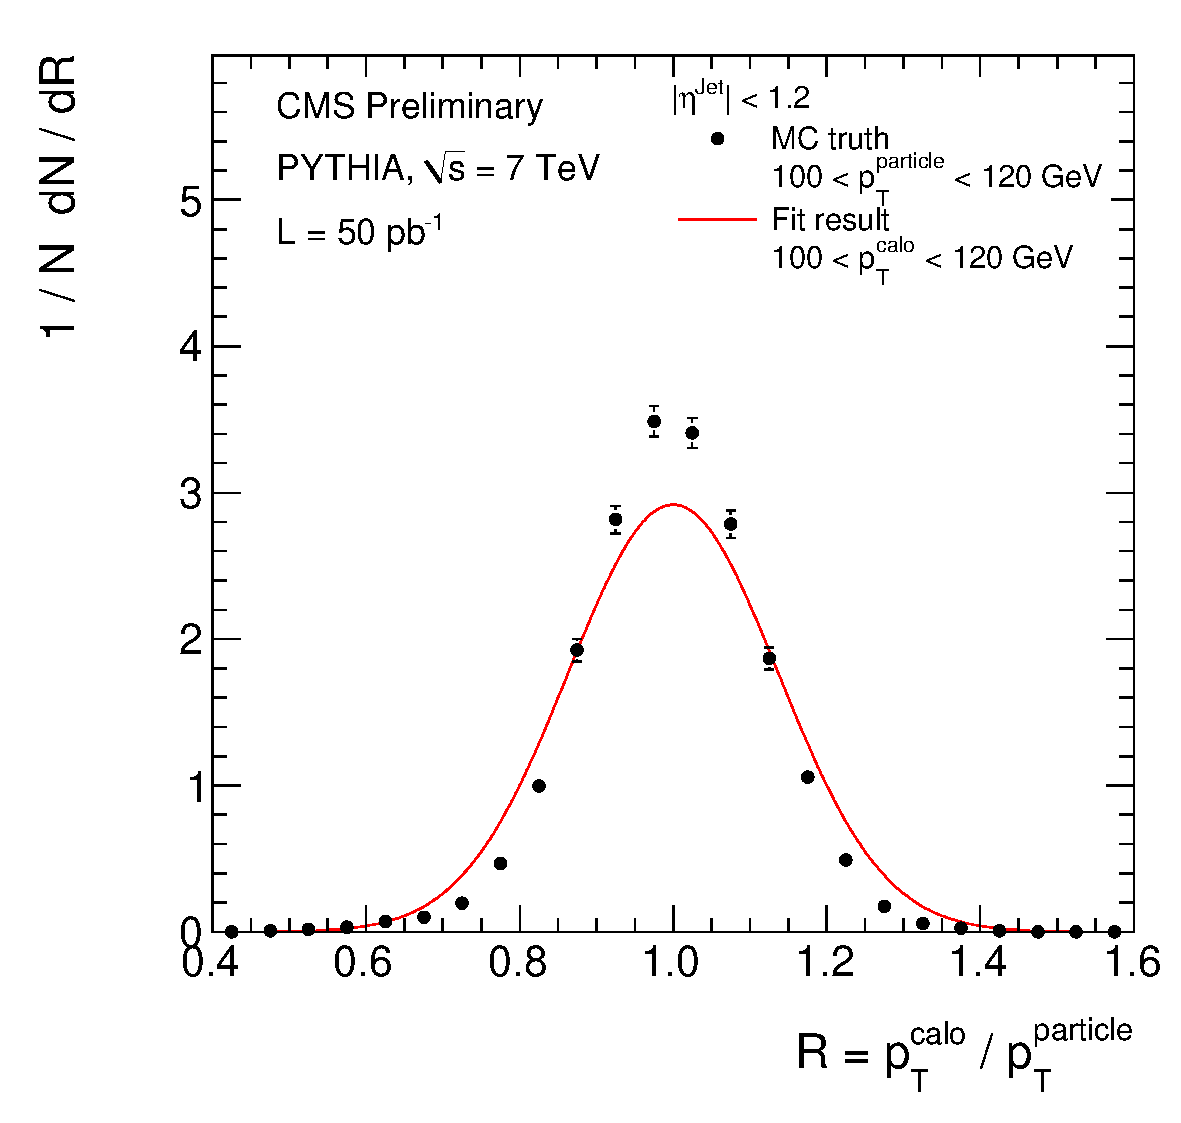
\includegraphics[width=0.3\textwidth]{figures/ResFit_Spring10QCDFlat_Gauss_Eta0_MCClosure_PtBin1} &
    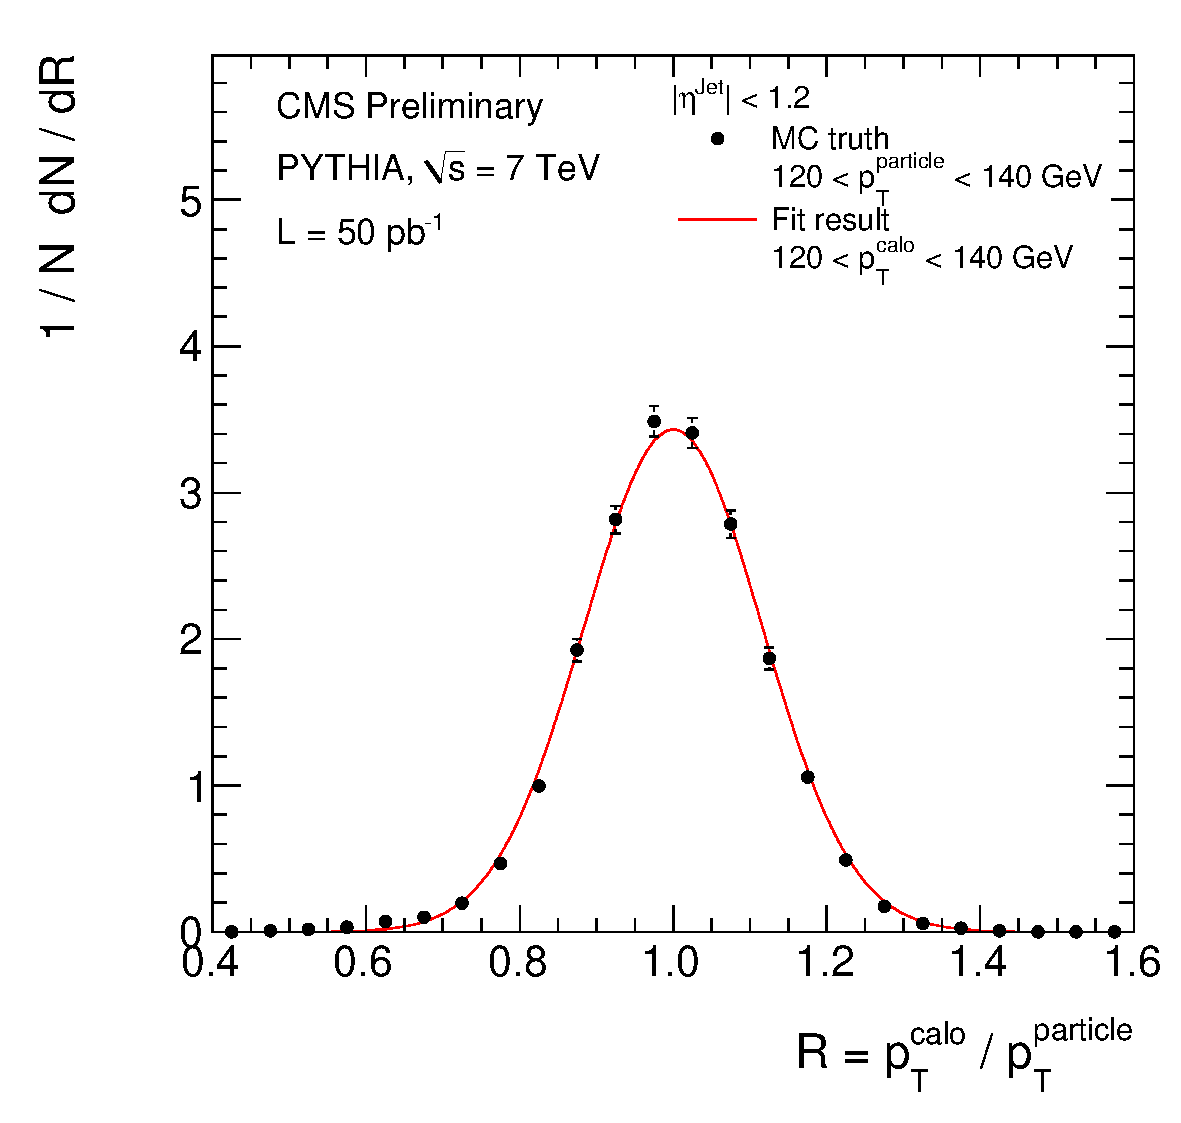
\includegraphics[width=0.3\textwidth]{figures/ResFit_Spring10QCDFlat_Gauss_Eta0_MCClosure_PtBin2} &
    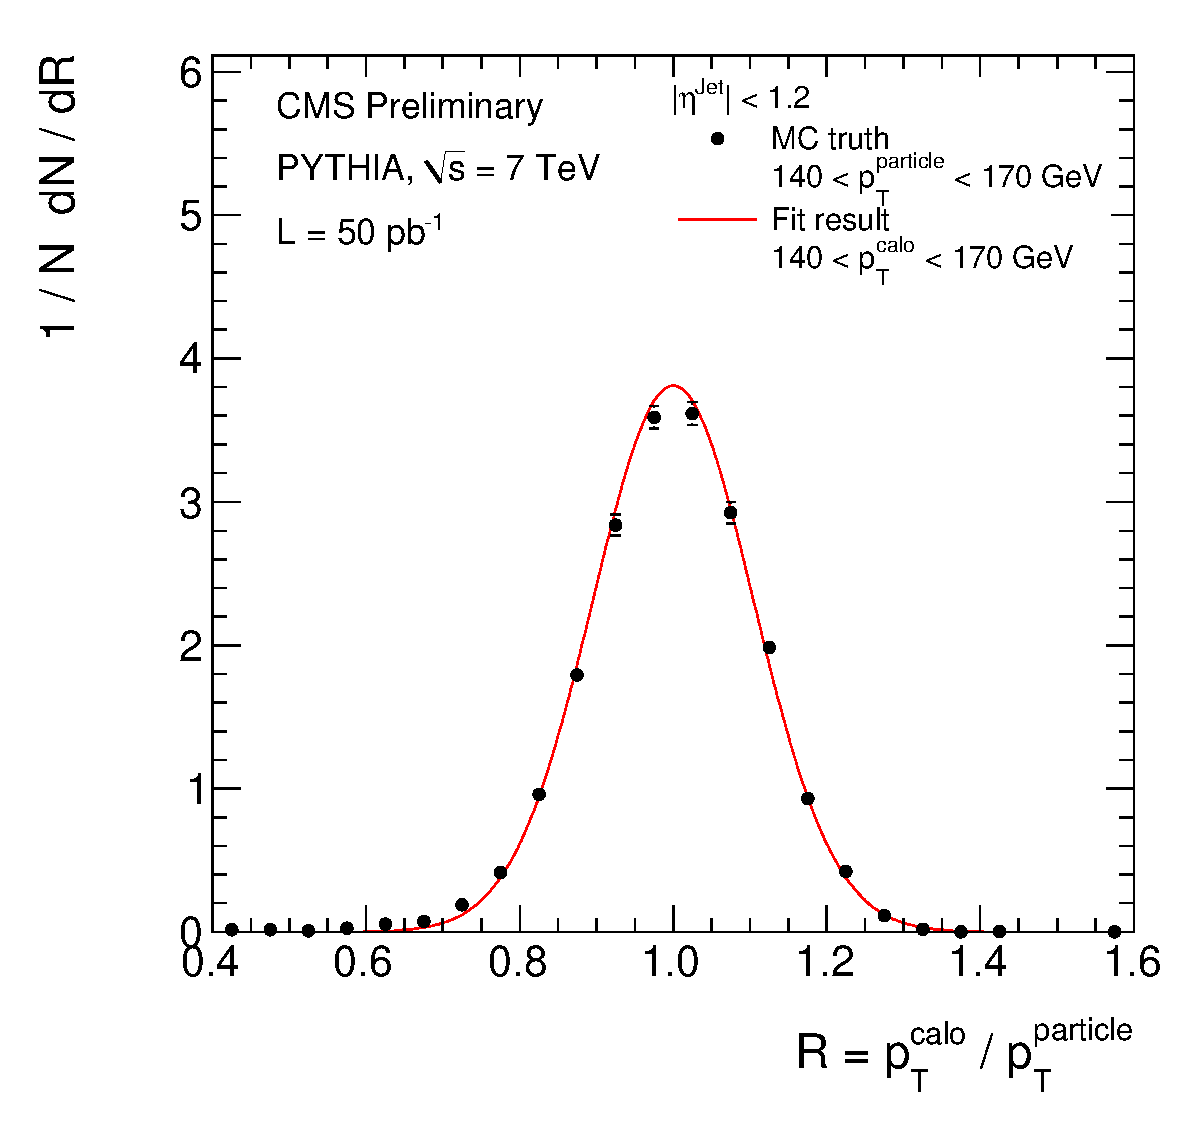
\includegraphics[width=0.3\textwidth]{figures/ResFit_Spring10QCDFlat_Gauss_Eta0_MCClosure_PtBin3} \\

    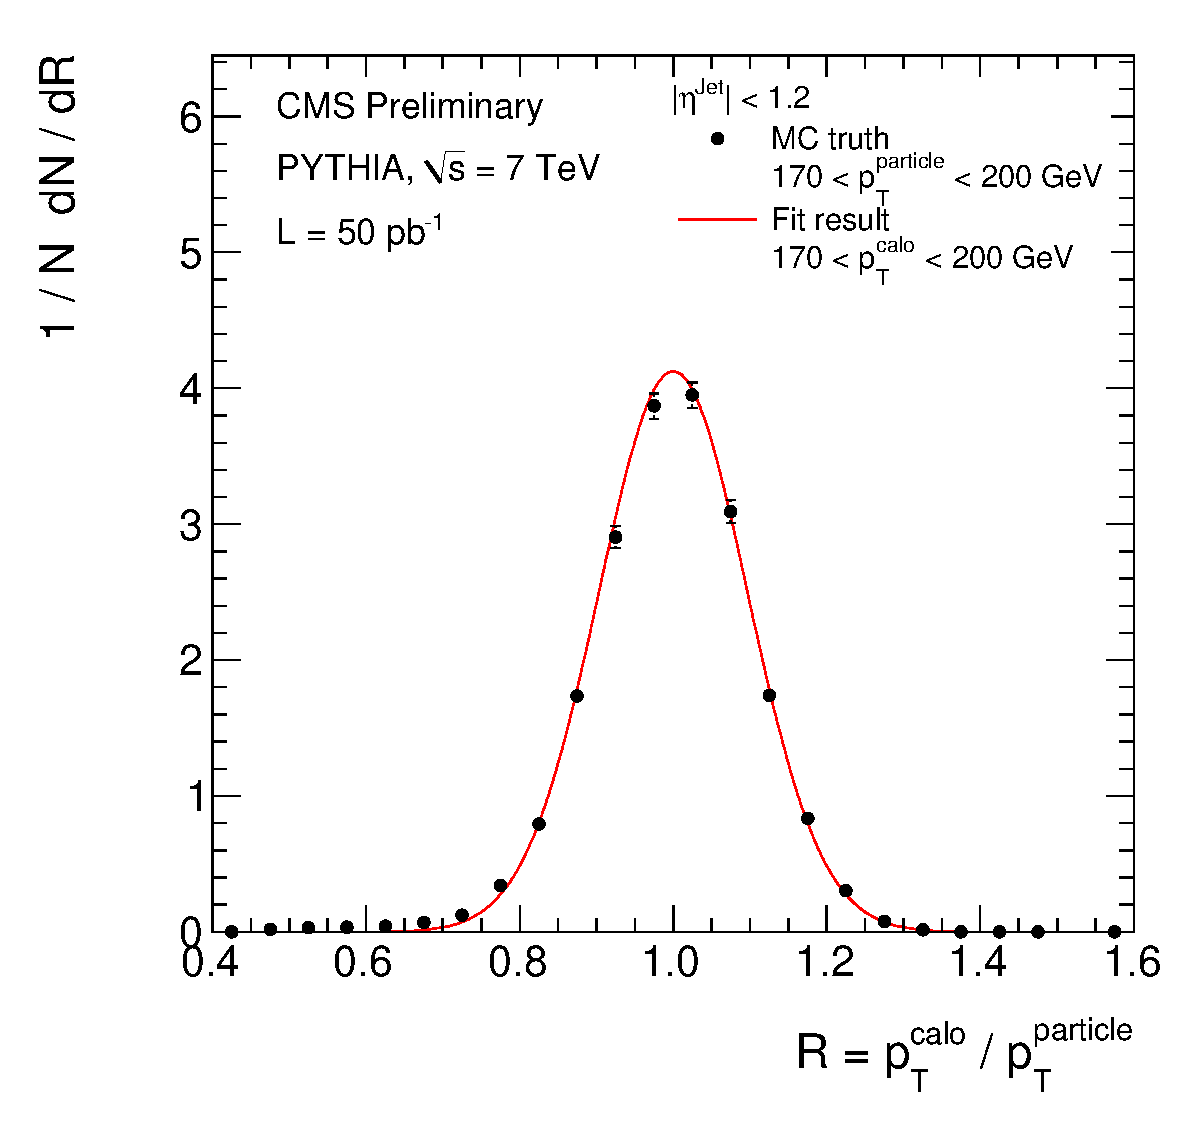
\includegraphics[width=0.3\textwidth]{figures/ResFit_Spring10QCDFlat_Gauss_Eta0_MCClosure_PtBin4} &
    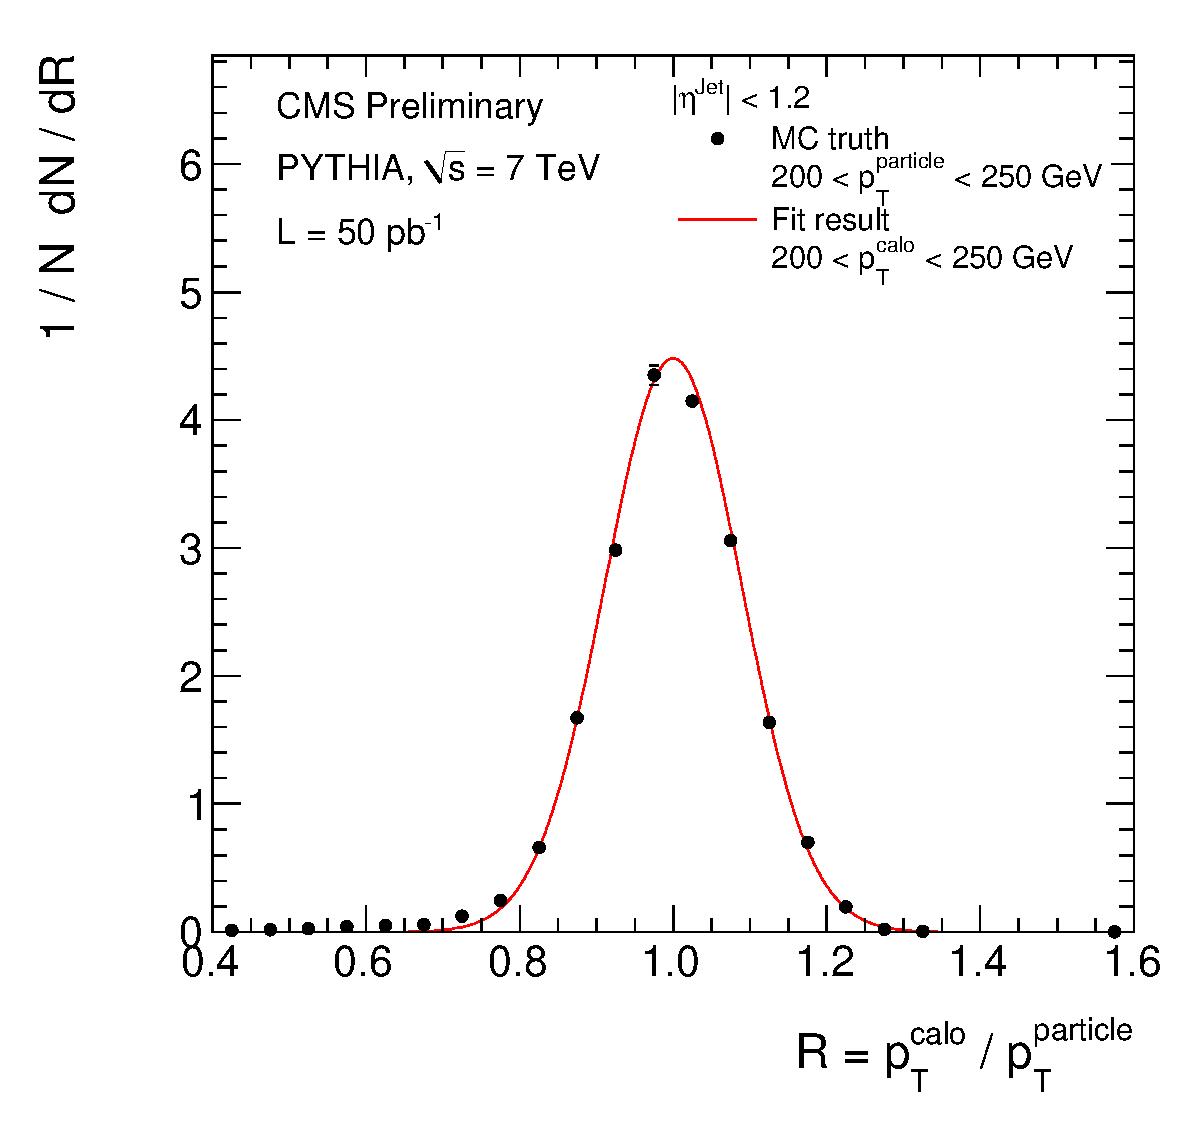
\includegraphics[width=0.3\textwidth]{figures/ResFit_Spring10QCDFlat_Gauss_Eta0_MCClosure_PtBin5} &
    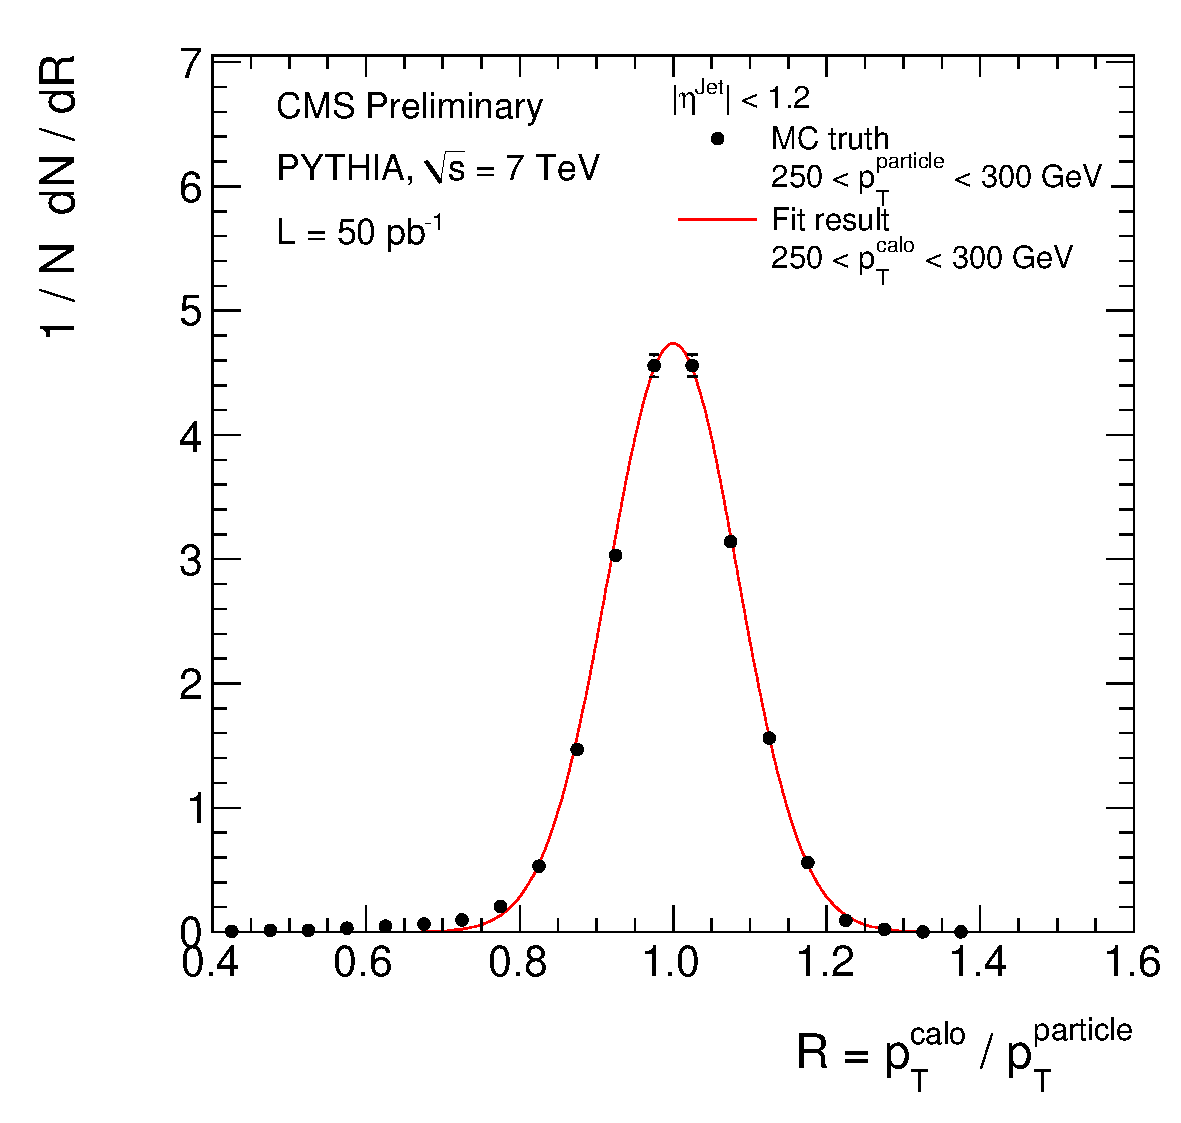
\includegraphics[width=0.3\textwidth]{figures/ResFit_Spring10QCDFlat_Gauss_Eta0_MCClosure_PtBin6} \\

    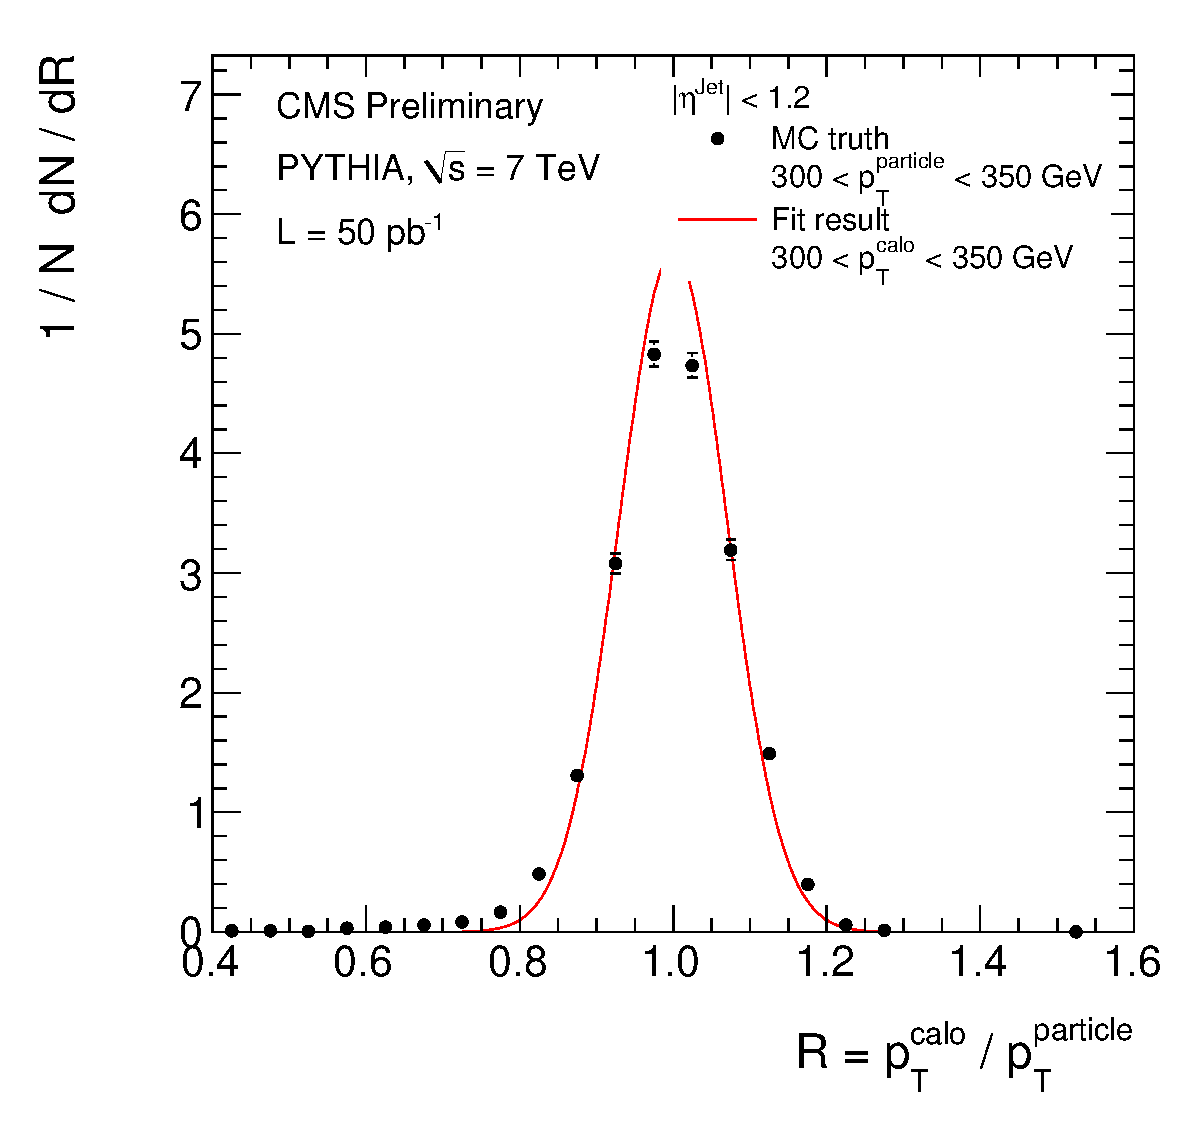
\includegraphics[width=0.3\textwidth]{figures/ResFit_Spring10QCDFlat_Gauss_Eta0_MCClosure_PtBin7} &
    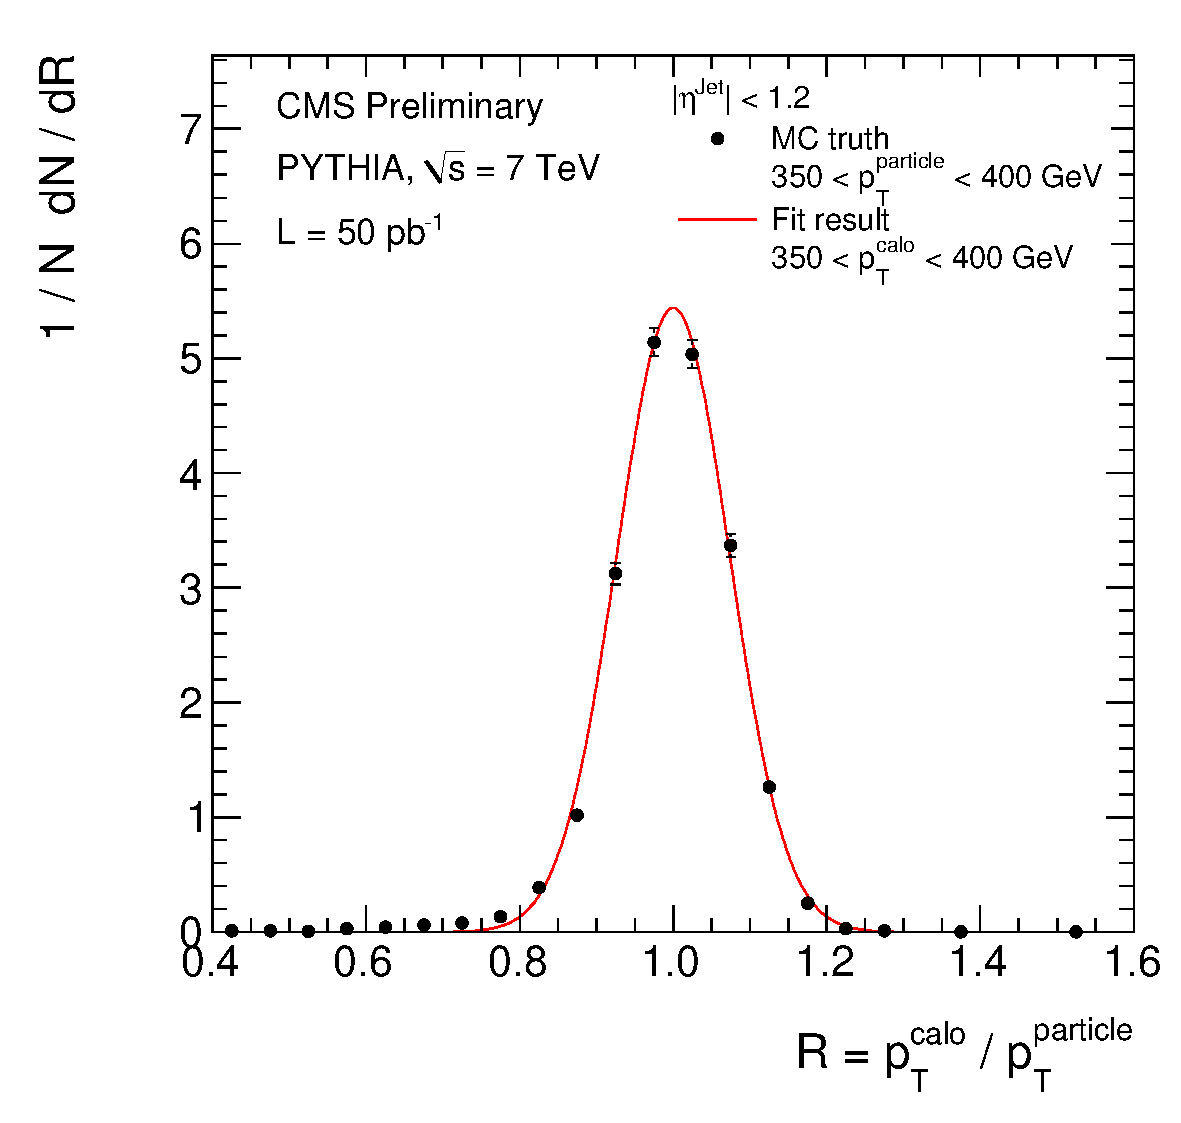
\includegraphics[width=0.3\textwidth]{figures/ResFit_Spring10QCDFlat_Gauss_Eta0_MCClosure_PtBin8} &
    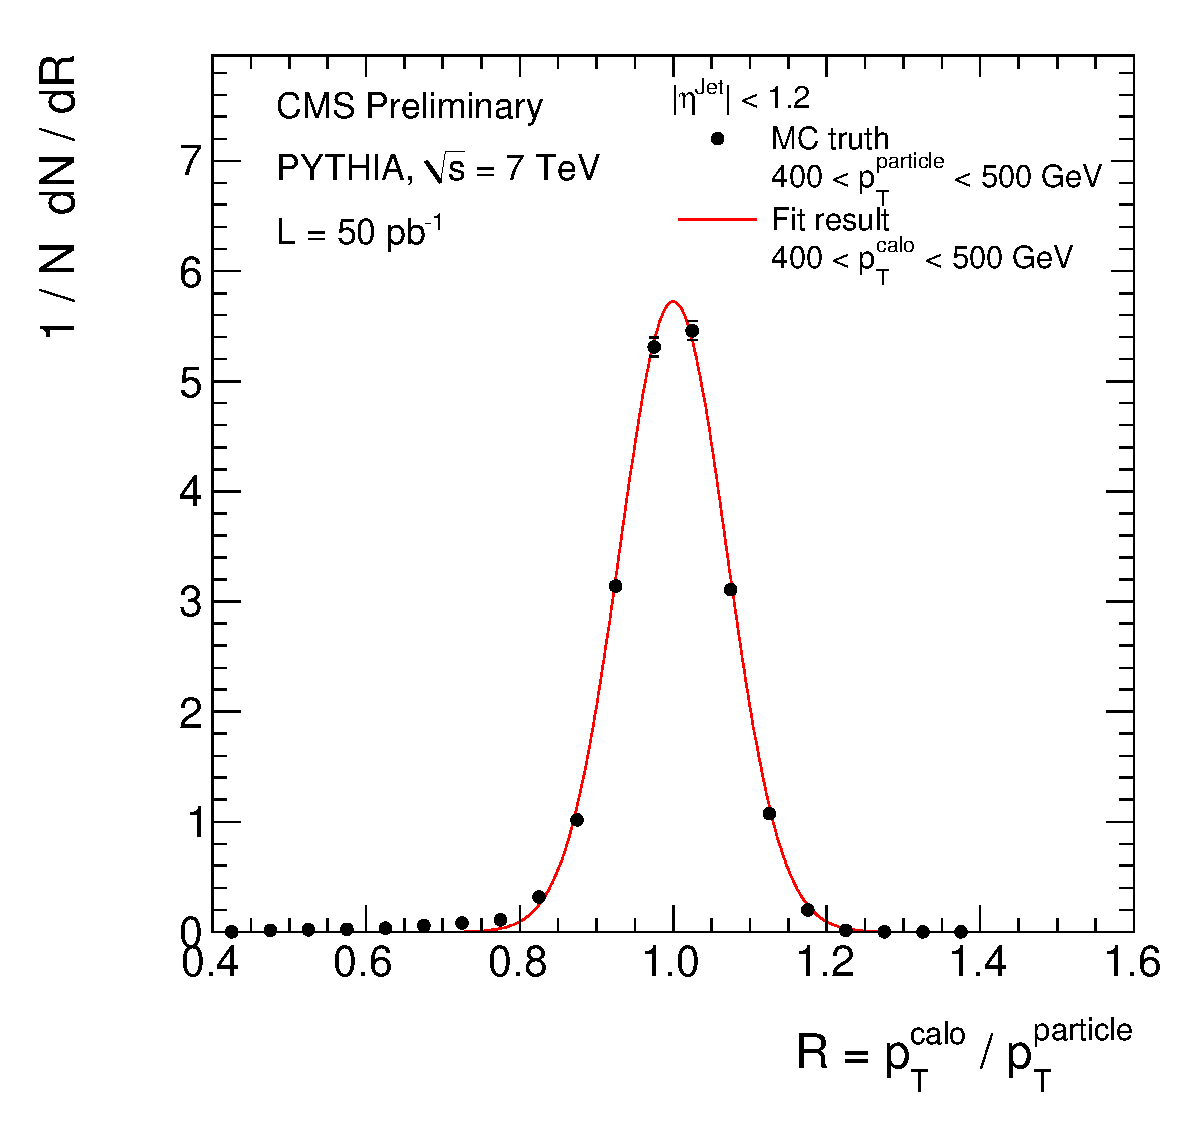
\includegraphics[width=0.3\textwidth]{figures/ResFit_Spring10QCDFlat_Gauss_Eta0_MCClosure_PtBin9} \\

    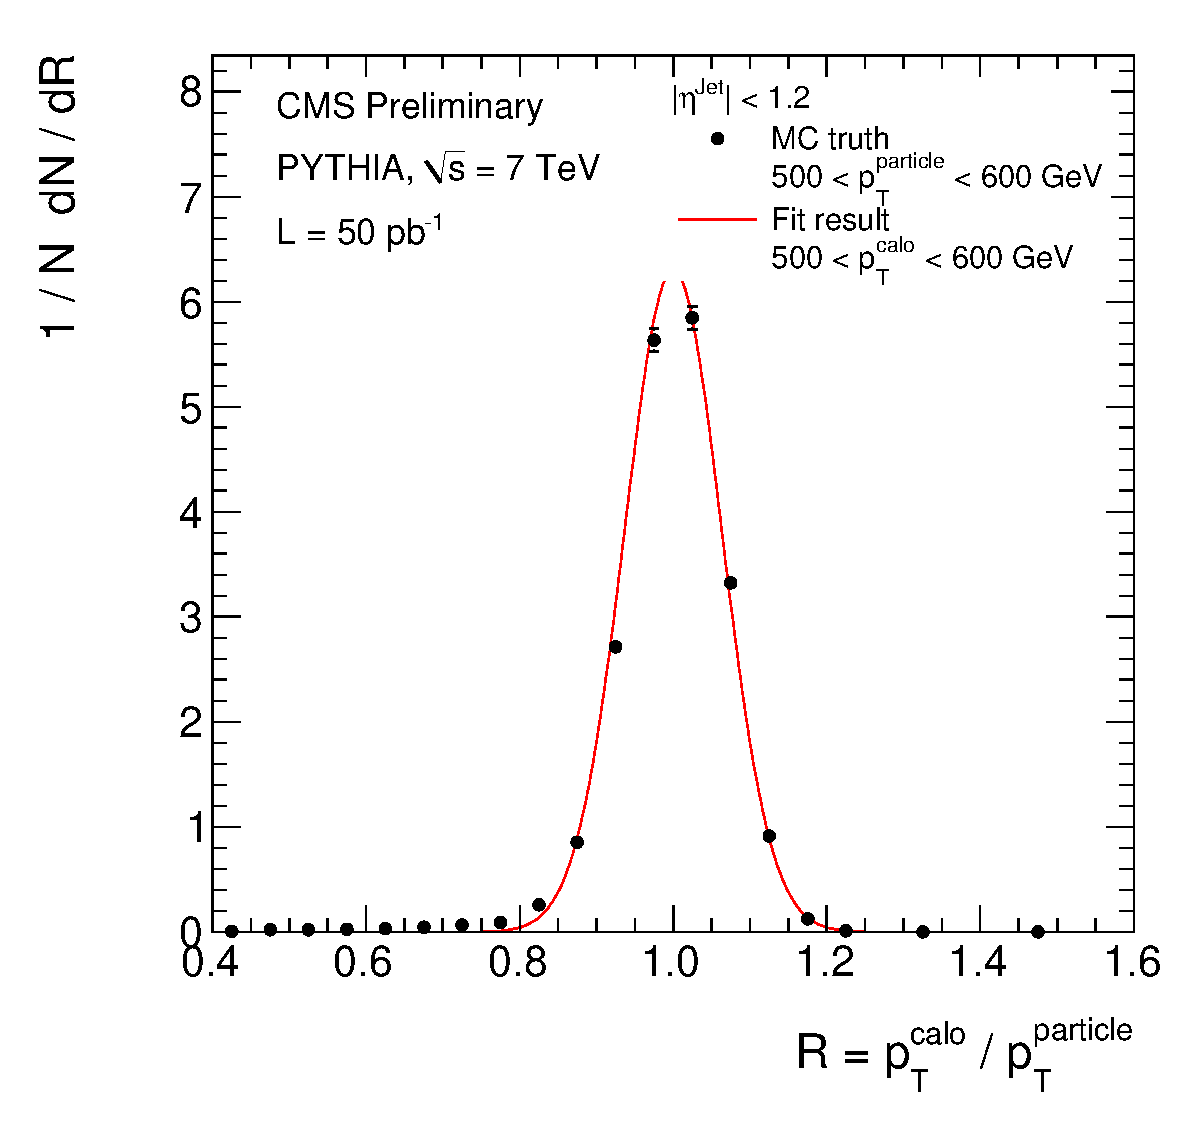
\includegraphics[width=0.3\textwidth]{figures/ResFit_Spring10QCDFlat_Gauss_Eta0_MCClosure_PtBin10} &
    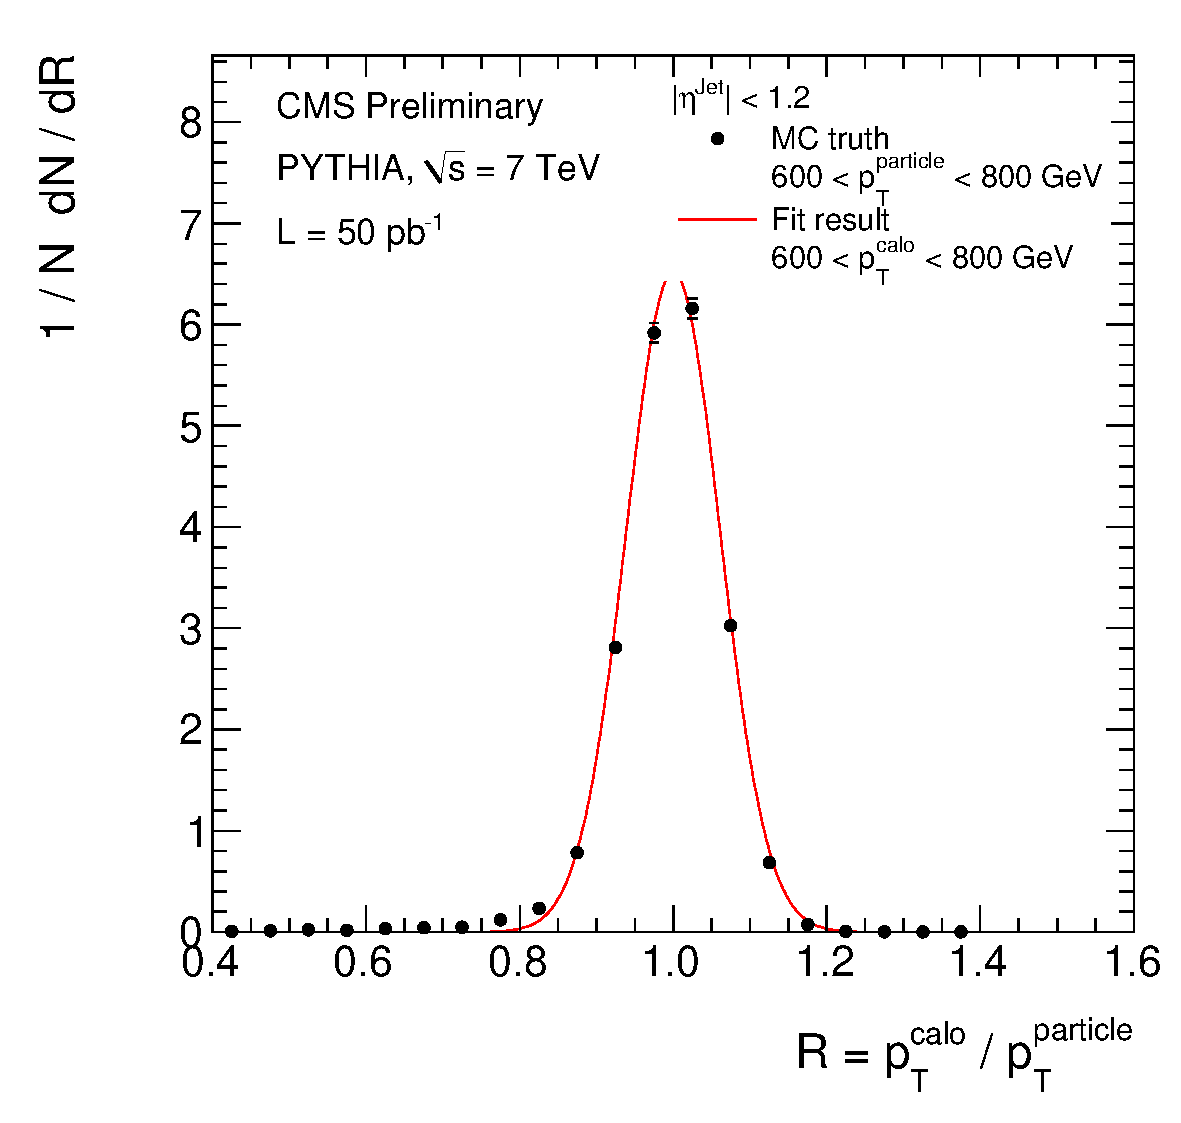
\includegraphics[width=0.3\textwidth]{figures/ResFit_Spring10QCDFlat_Gauss_Eta0_MCClosure_PtBin11} &
    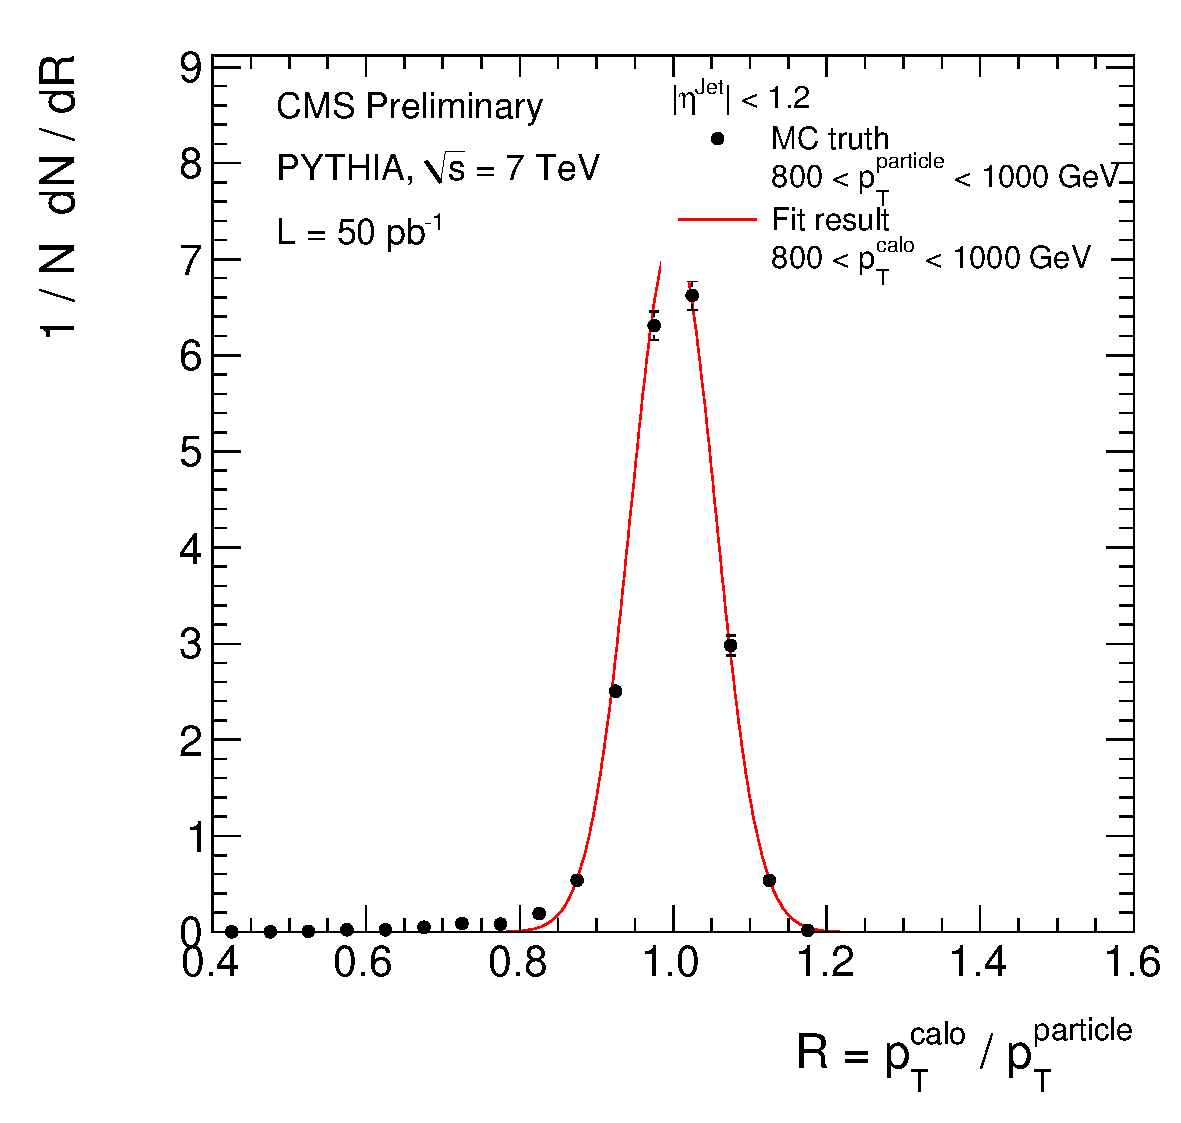
\includegraphics[width=0.3\textwidth]{figures/ResFit_Spring10QCDFlat_Gauss_Eta0_MCClosure_PtBin12} \\
  \end{tabular}
\caption{Closure \mbox{$|\eta|<1.2$}.}
\label{fig:ResFit:App:Gauss:MCClosure}
\end{figure}

\clearpage


\subsection{Crystal Ball response function}\label{sec:ResFit:App:AllResults:CrystalBall}

% ----- Crystal Ball Eta0 Spectra -----
\begin{figure}[ht]
  \centering
  \begin{tabular}{ccc}
    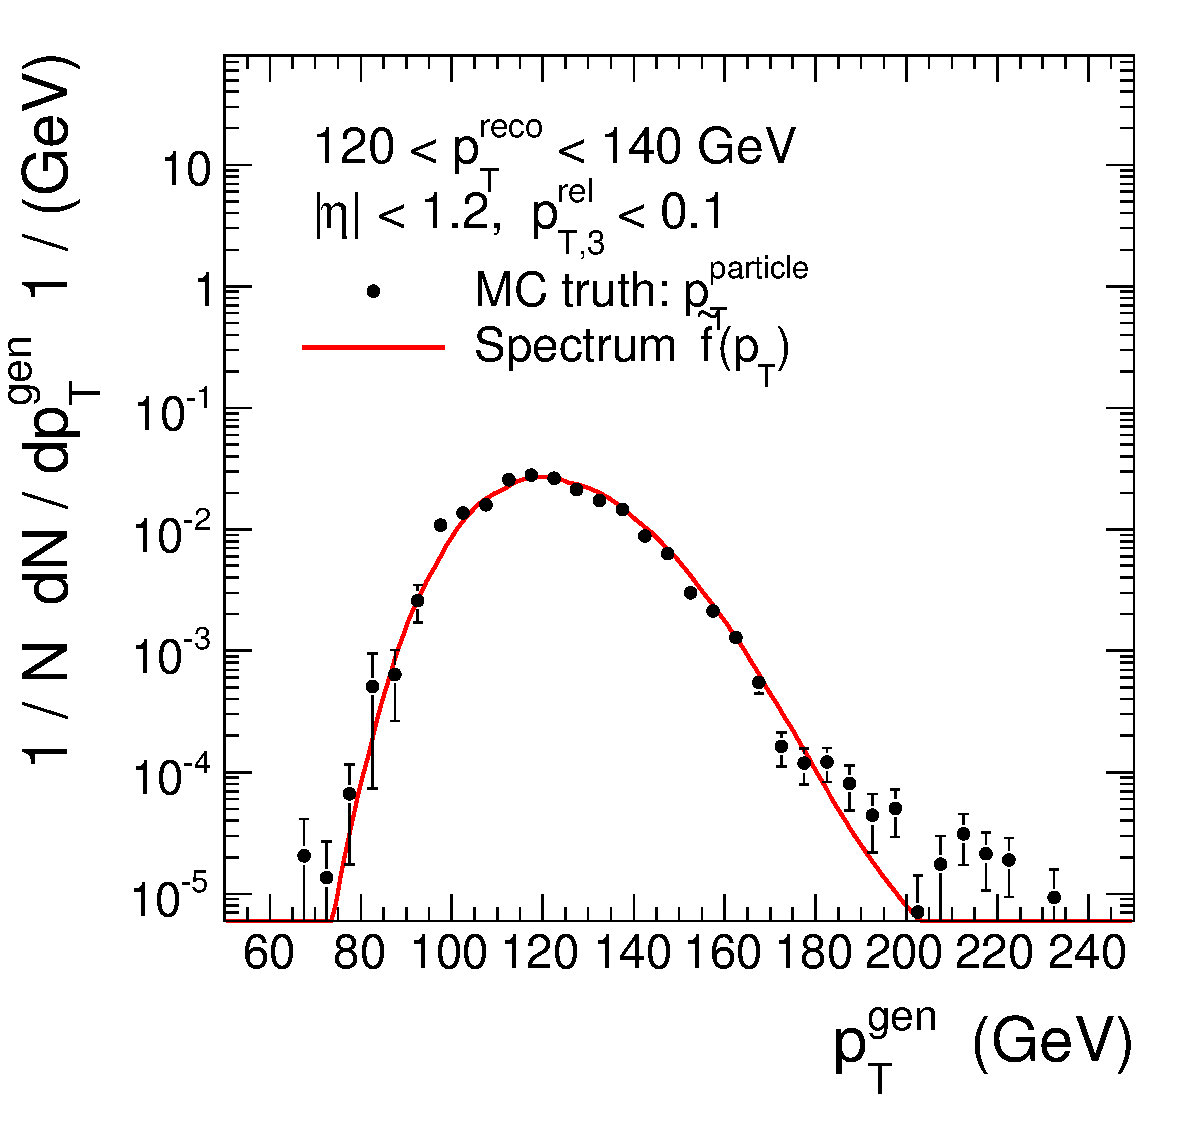
\includegraphics[width=0.3\textwidth]{figures/ResFit_Spring10QCDFlat_CB_Eta0_Spectrum_PtBin0} &
    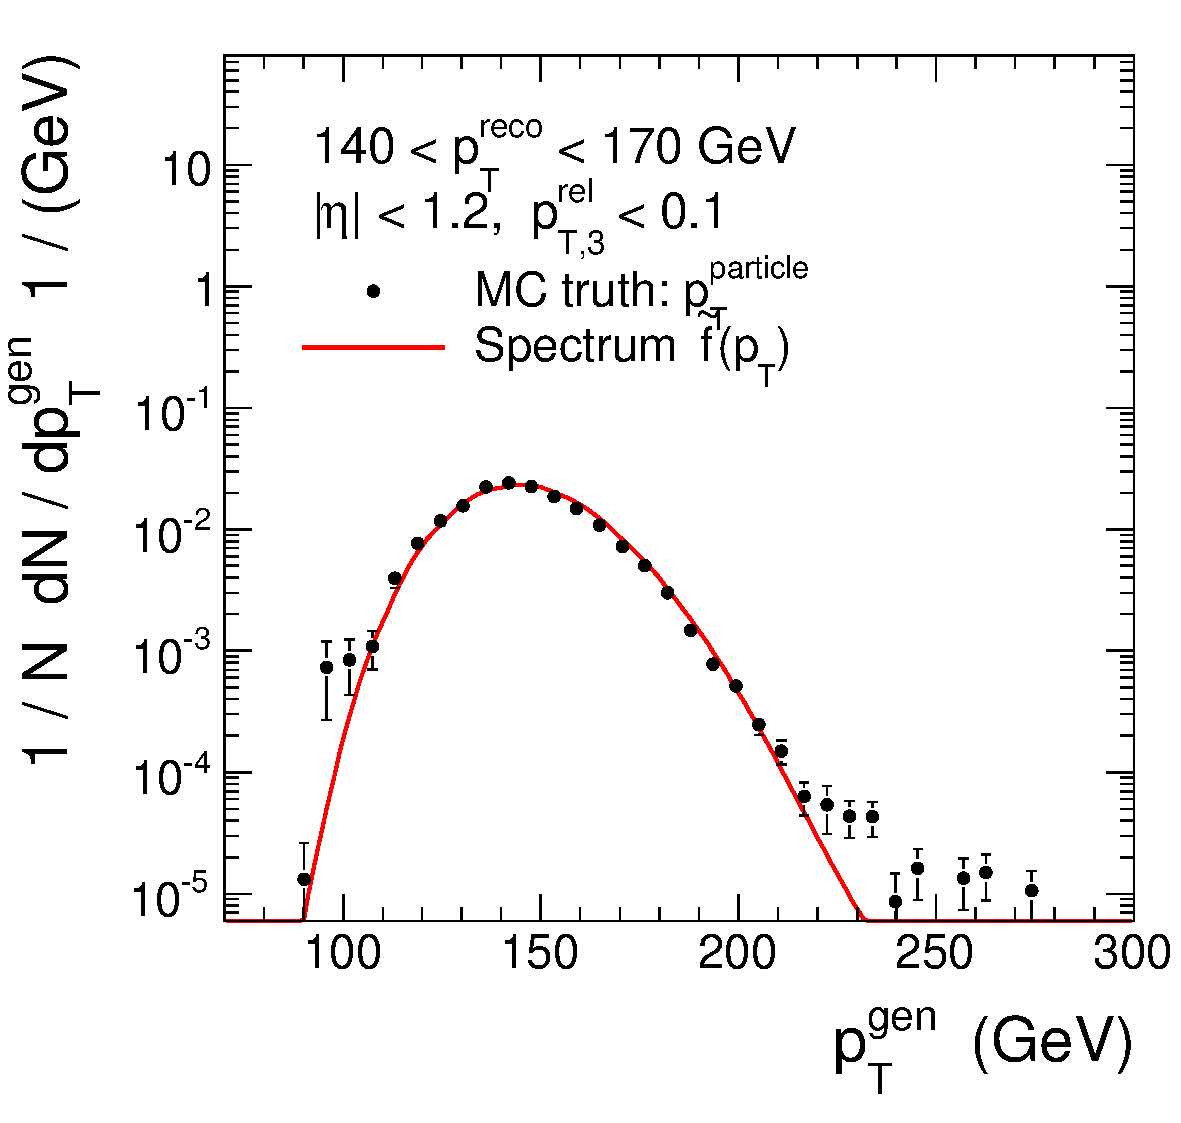
\includegraphics[width=0.3\textwidth]{figures/ResFit_Spring10QCDFlat_CB_Eta0_Spectrum_PtBin1} &
    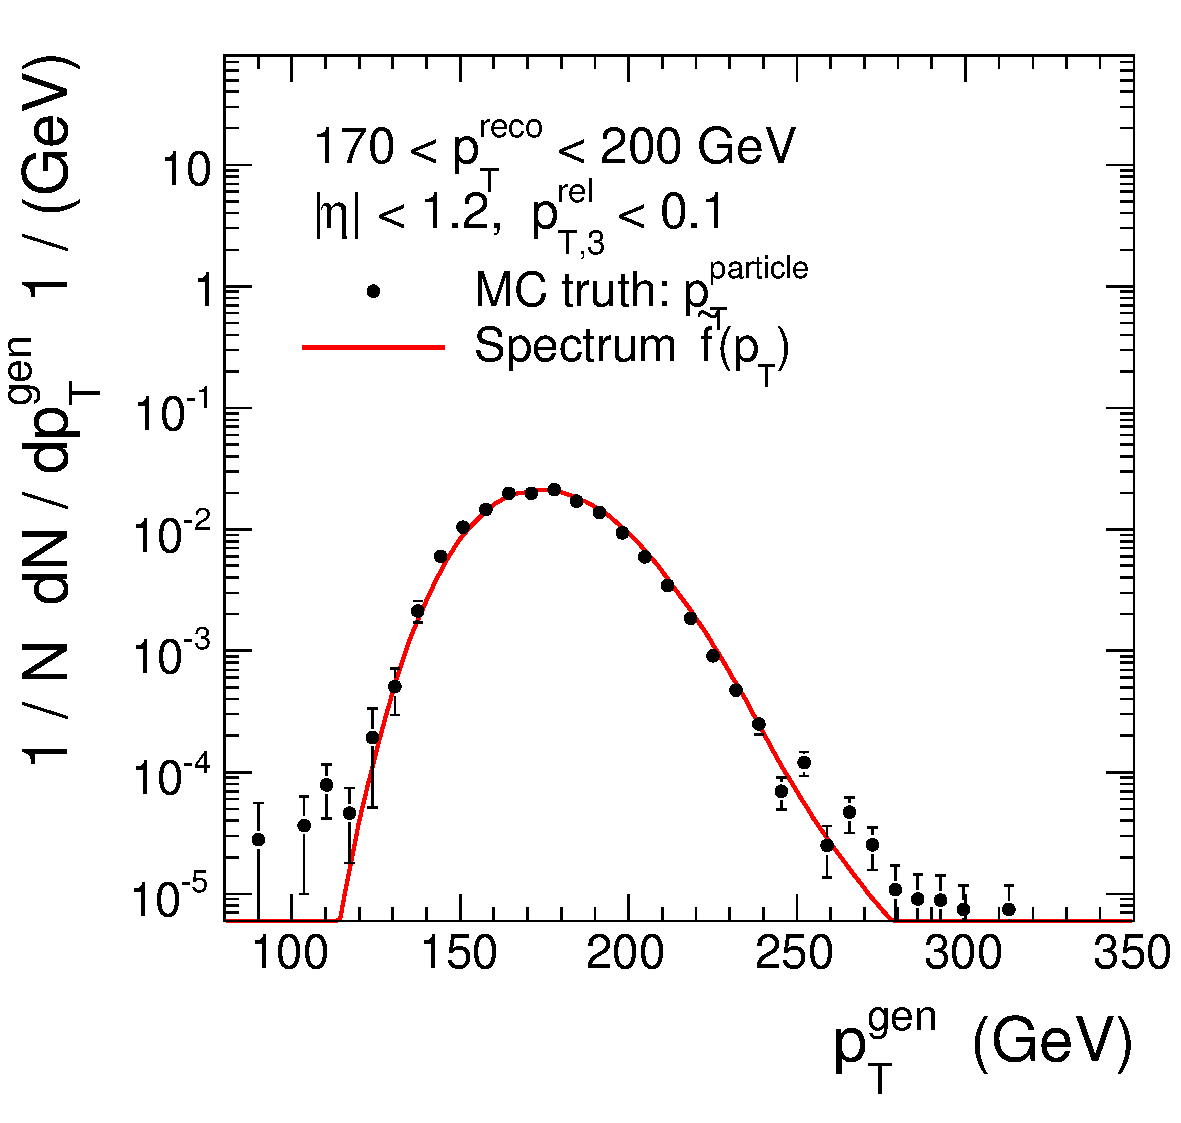
\includegraphics[width=0.3\textwidth]{figures/ResFit_Spring10QCDFlat_CB_Eta0_Spectrum_PtBin2} \\

    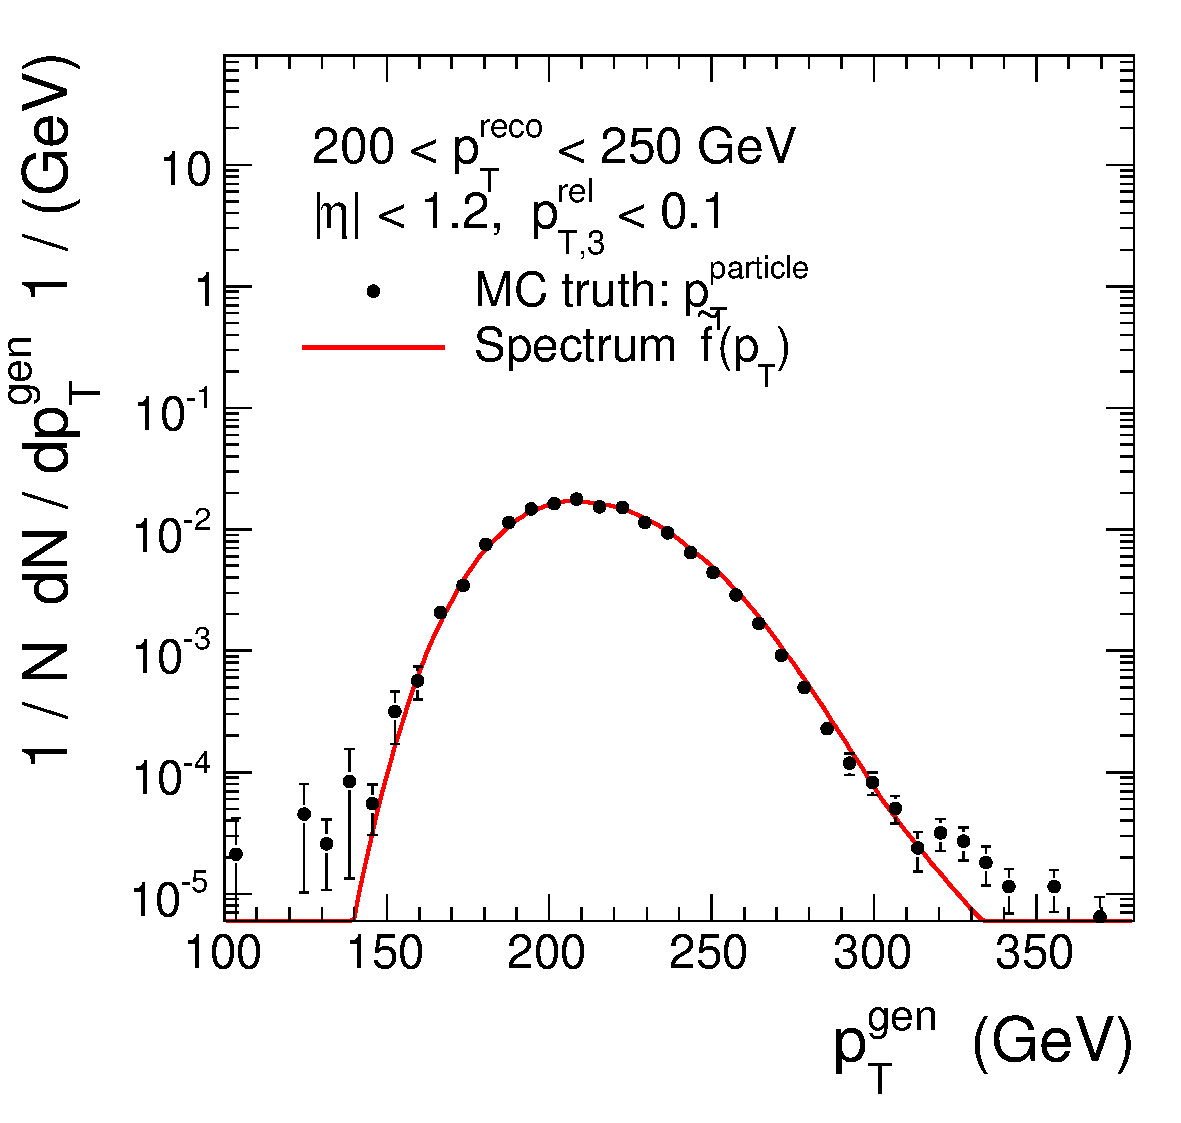
\includegraphics[width=0.3\textwidth]{figures/ResFit_Spring10QCDFlat_CB_Eta0_Spectrum_PtBin3} &
    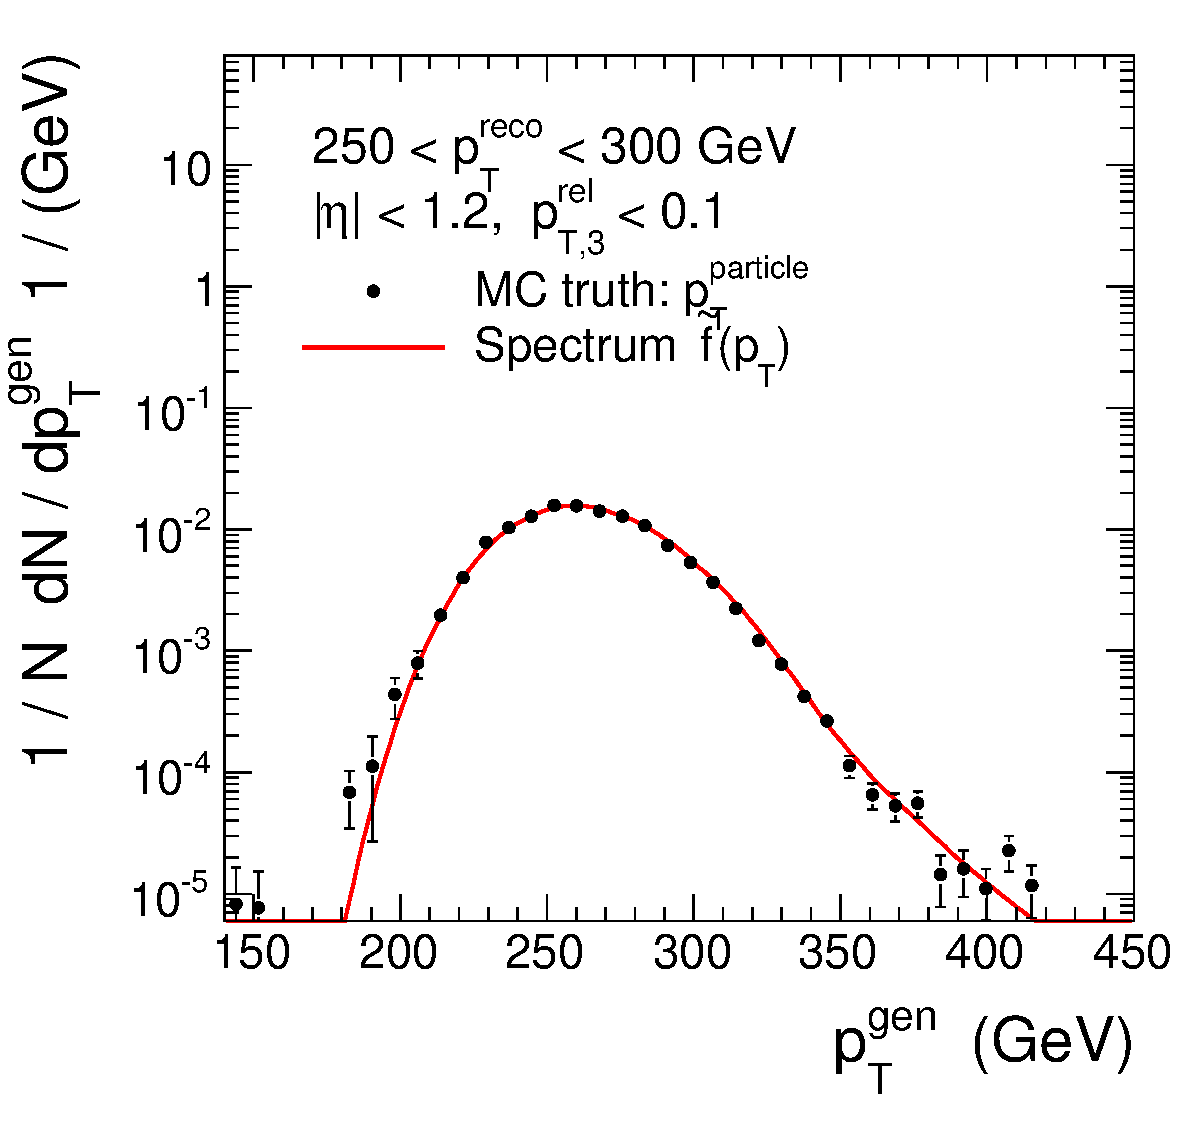
\includegraphics[width=0.3\textwidth]{figures/ResFit_Spring10QCDFlat_CB_Eta0_Spectrum_PtBin4} &
    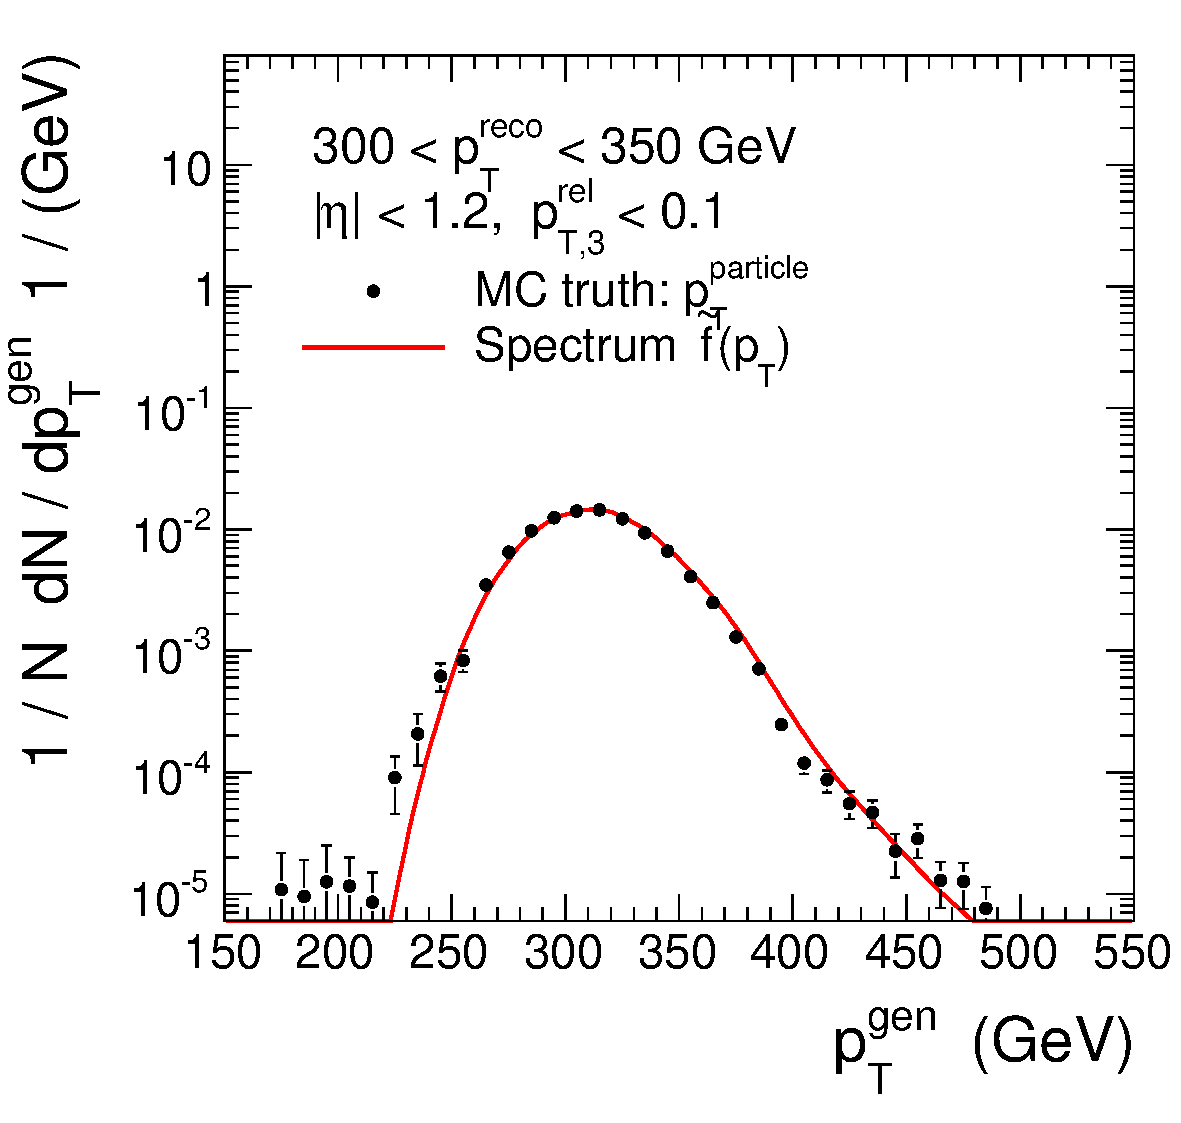
\includegraphics[width=0.3\textwidth]{figures/ResFit_Spring10QCDFlat_CB_Eta0_Spectrum_PtBin5} \\

    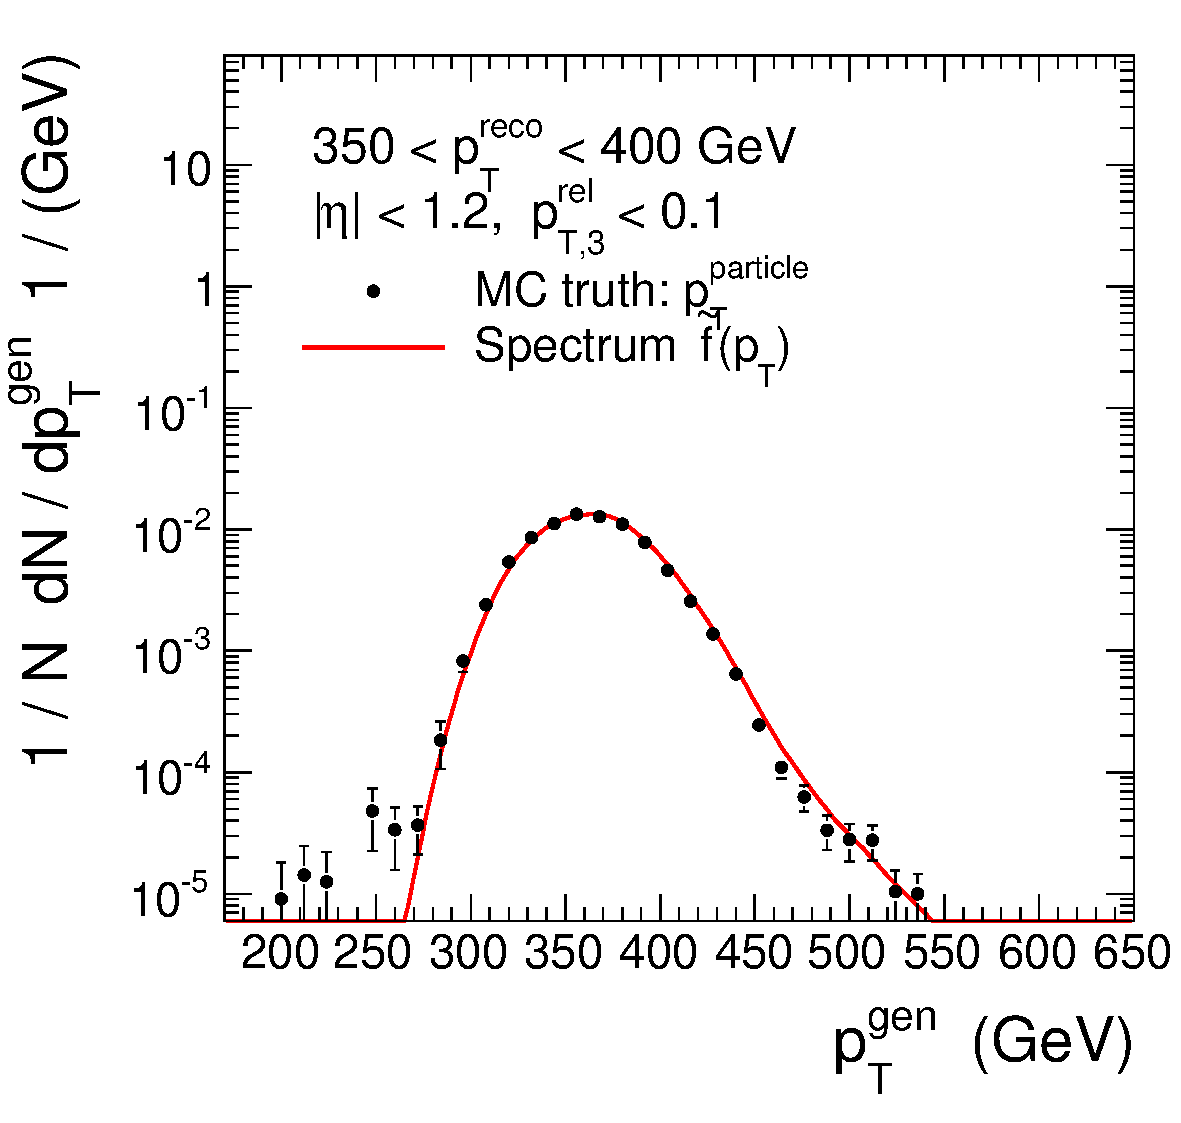
\includegraphics[width=0.3\textwidth]{figures/ResFit_Spring10QCDFlat_CB_Eta0_Spectrum_PtBin6} &
    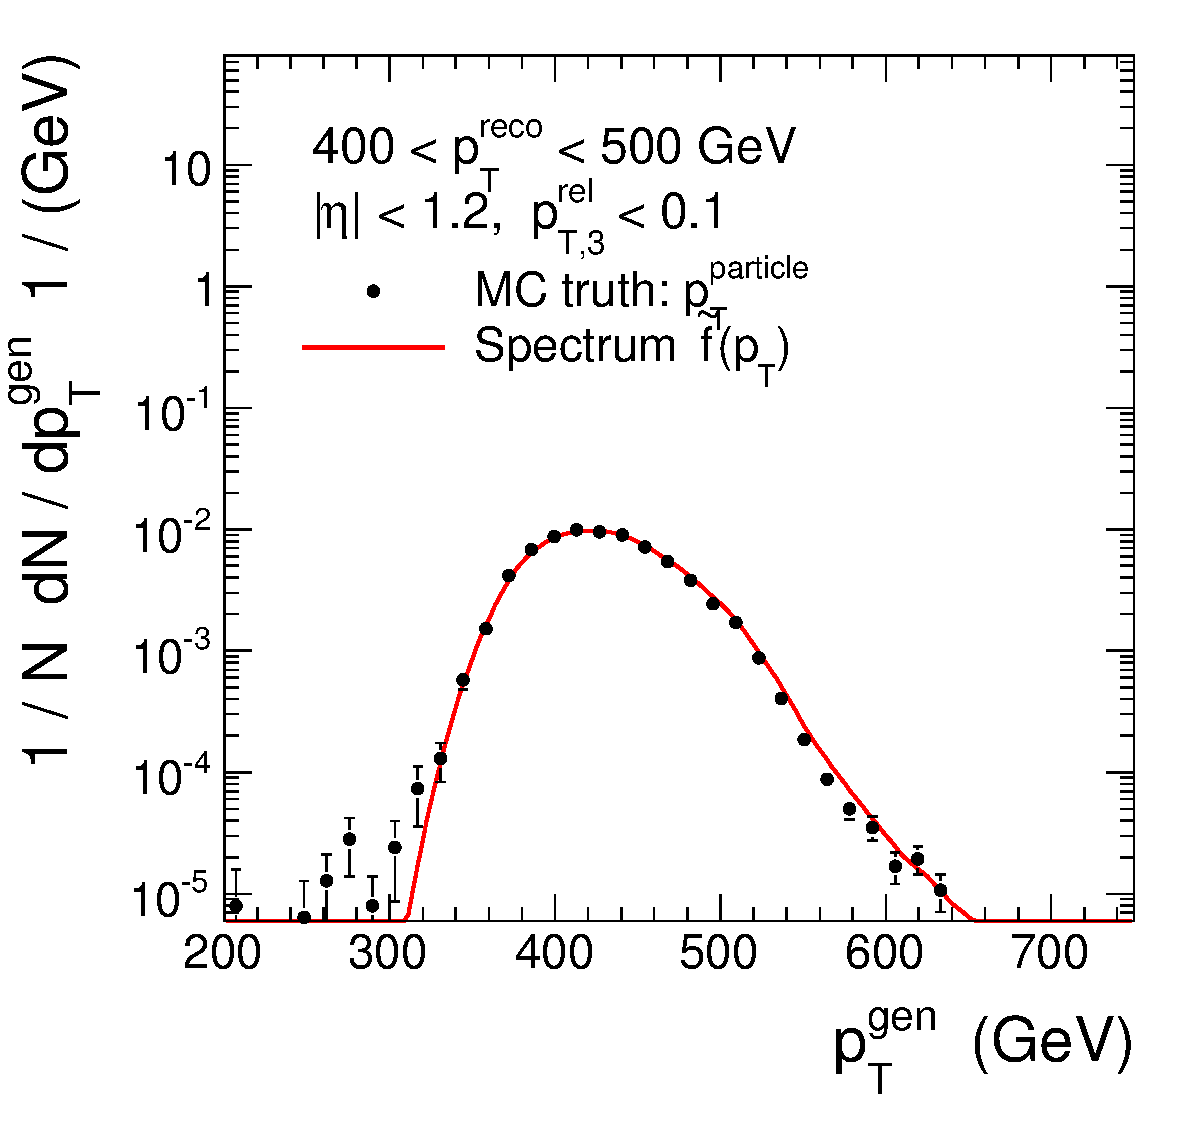
\includegraphics[width=0.3\textwidth]{figures/ResFit_Spring10QCDFlat_CB_Eta0_Spectrum_PtBin7} &
    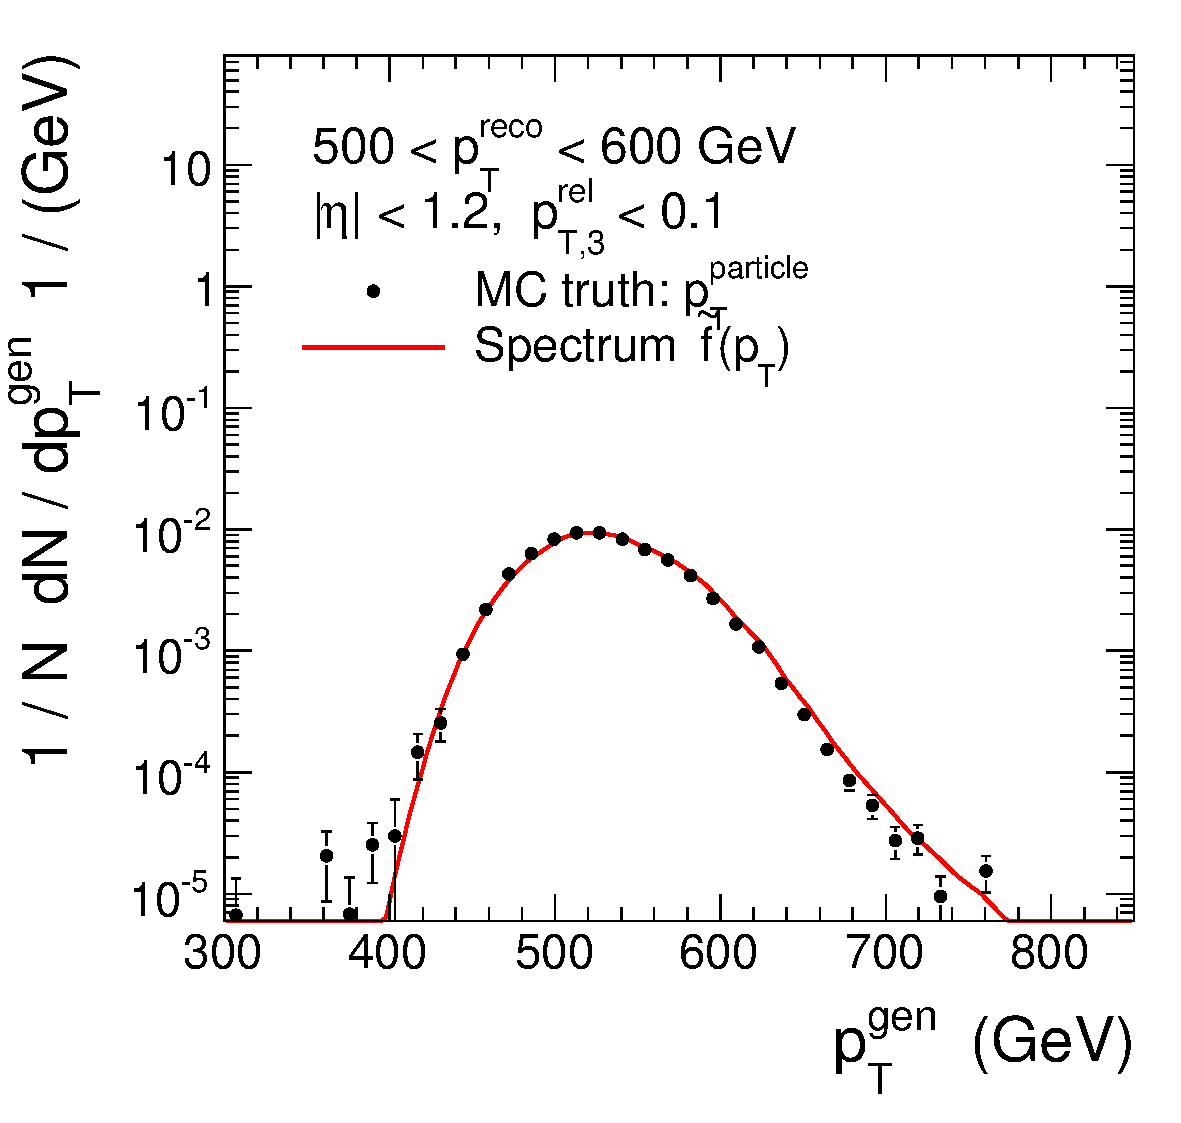
\includegraphics[width=0.3\textwidth]{figures/ResFit_Spring10QCDFlat_CB_Eta0_Spectrum_PtBin8} \\

    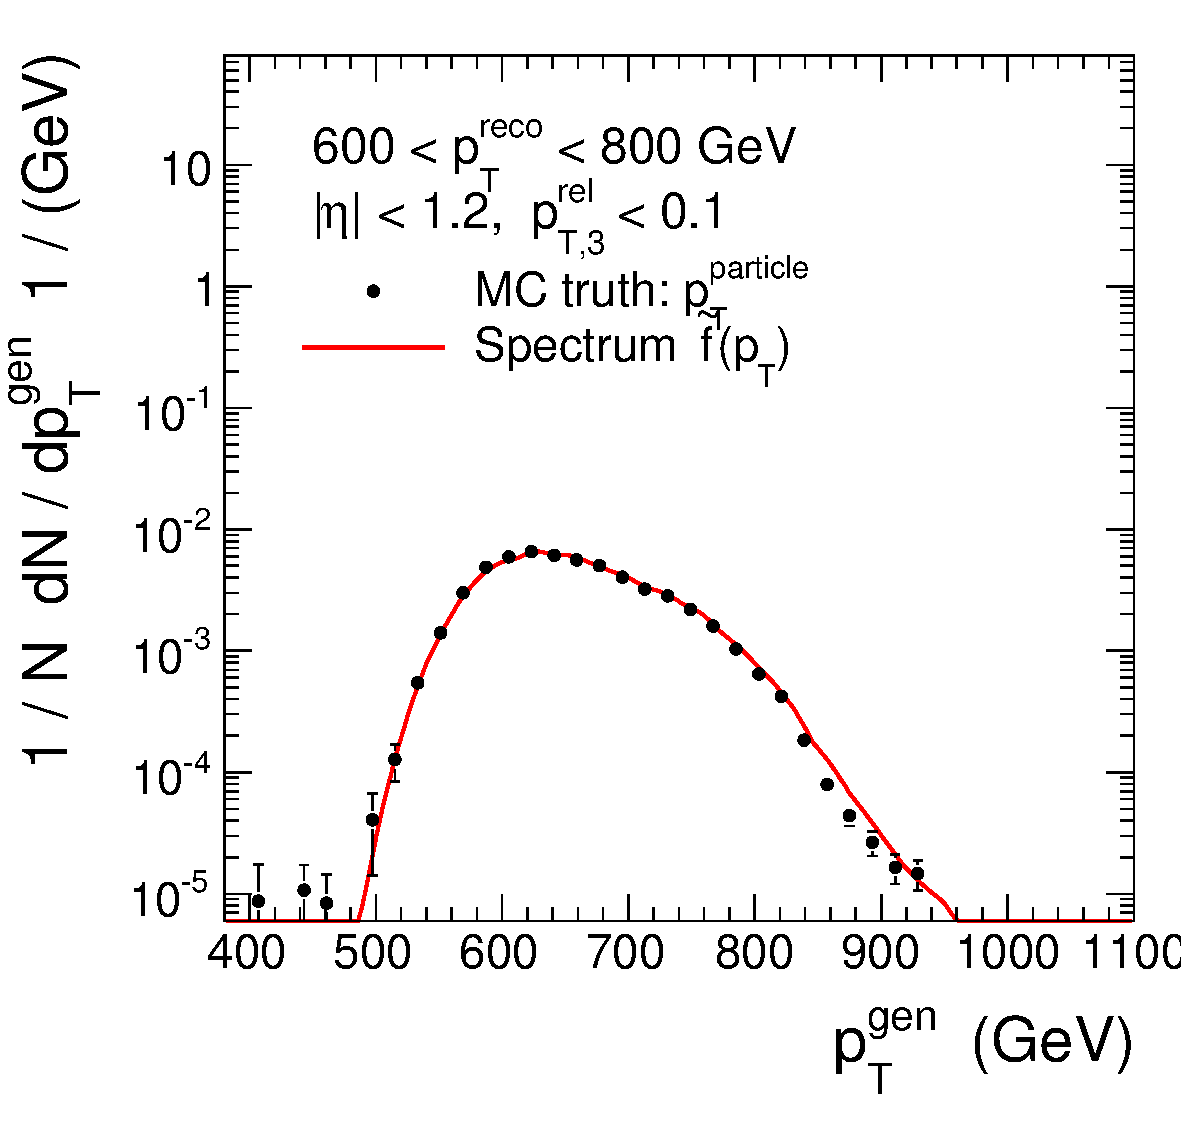
\includegraphics[width=0.3\textwidth]{figures/ResFit_Spring10QCDFlat_CB_Eta0_Spectrum_PtBin9} &
    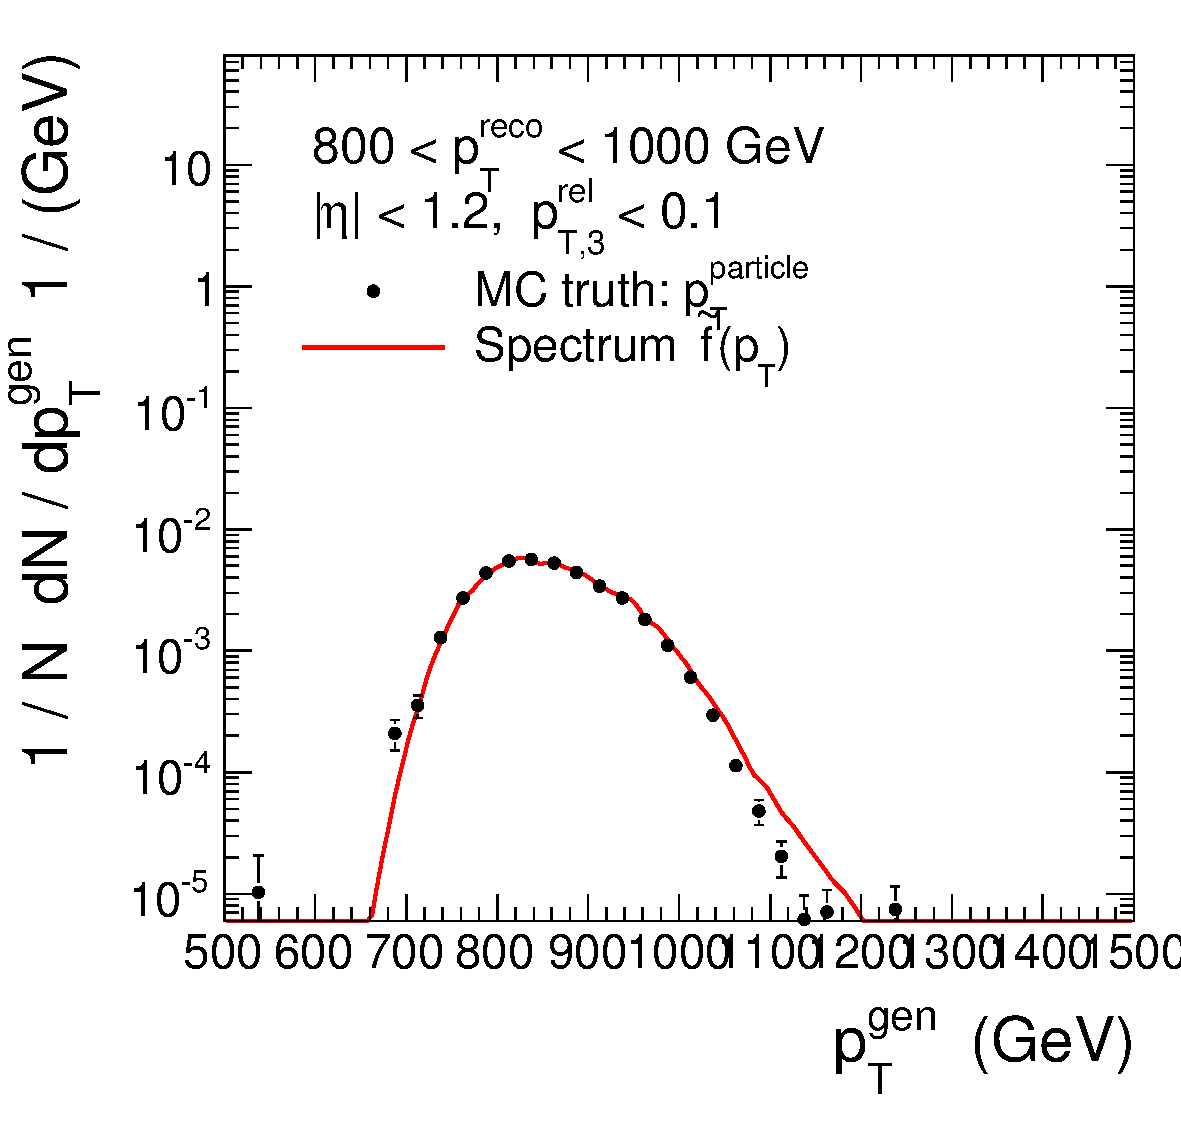
\includegraphics[width=0.3\textwidth]{figures/ResFit_Spring10QCDFlat_CB_Eta0_Spectrum_PtBin10} & \\
  \end{tabular}
\caption{The parameterisation of the realistic particle jet \pt spectrum as used in the dijet likelihood (solid line) in comparison to the prediction from Monte Carlo truth (full circles) in different \pt bins for \mbox{$|\eta|<1.2$}. Migration effects are modeled assuming a Crystal Ball response function.}
\label{fig:ResFit:App:CB:Spectrum}
\end{figure}


% ----- Crystal Ball Eta0 extrapolations -----
\begin{figure}[ht]
  \centering
  \begin{tabular}{ccc}
    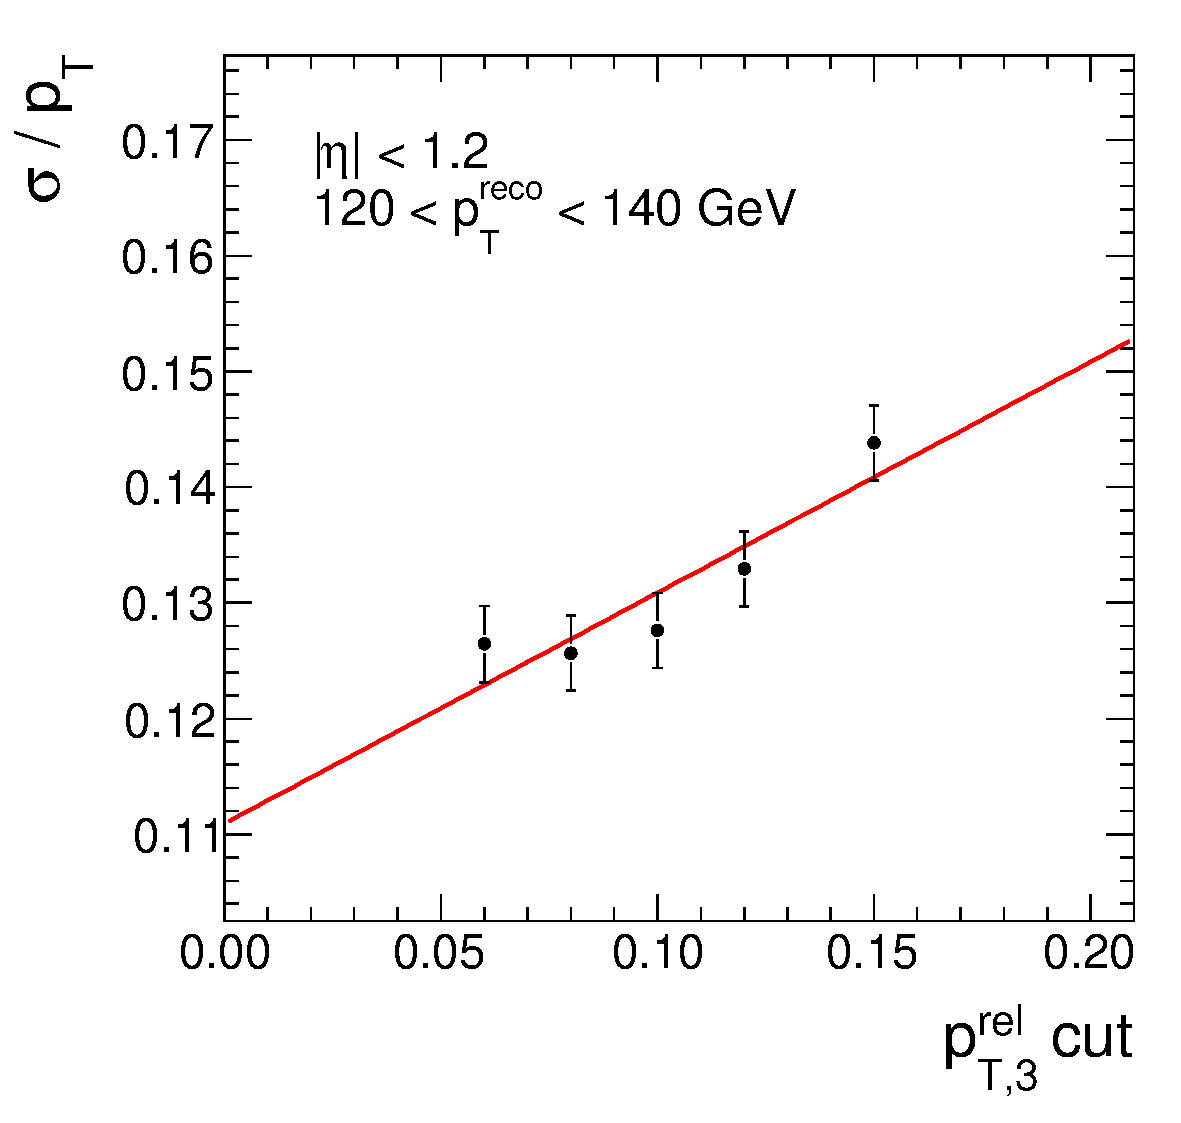
\includegraphics[width=0.3\textwidth]{figures/ResFit_Spring10QCDFlat_CB_Eta0_ExtrapolatedPar0_PtBin0} &
    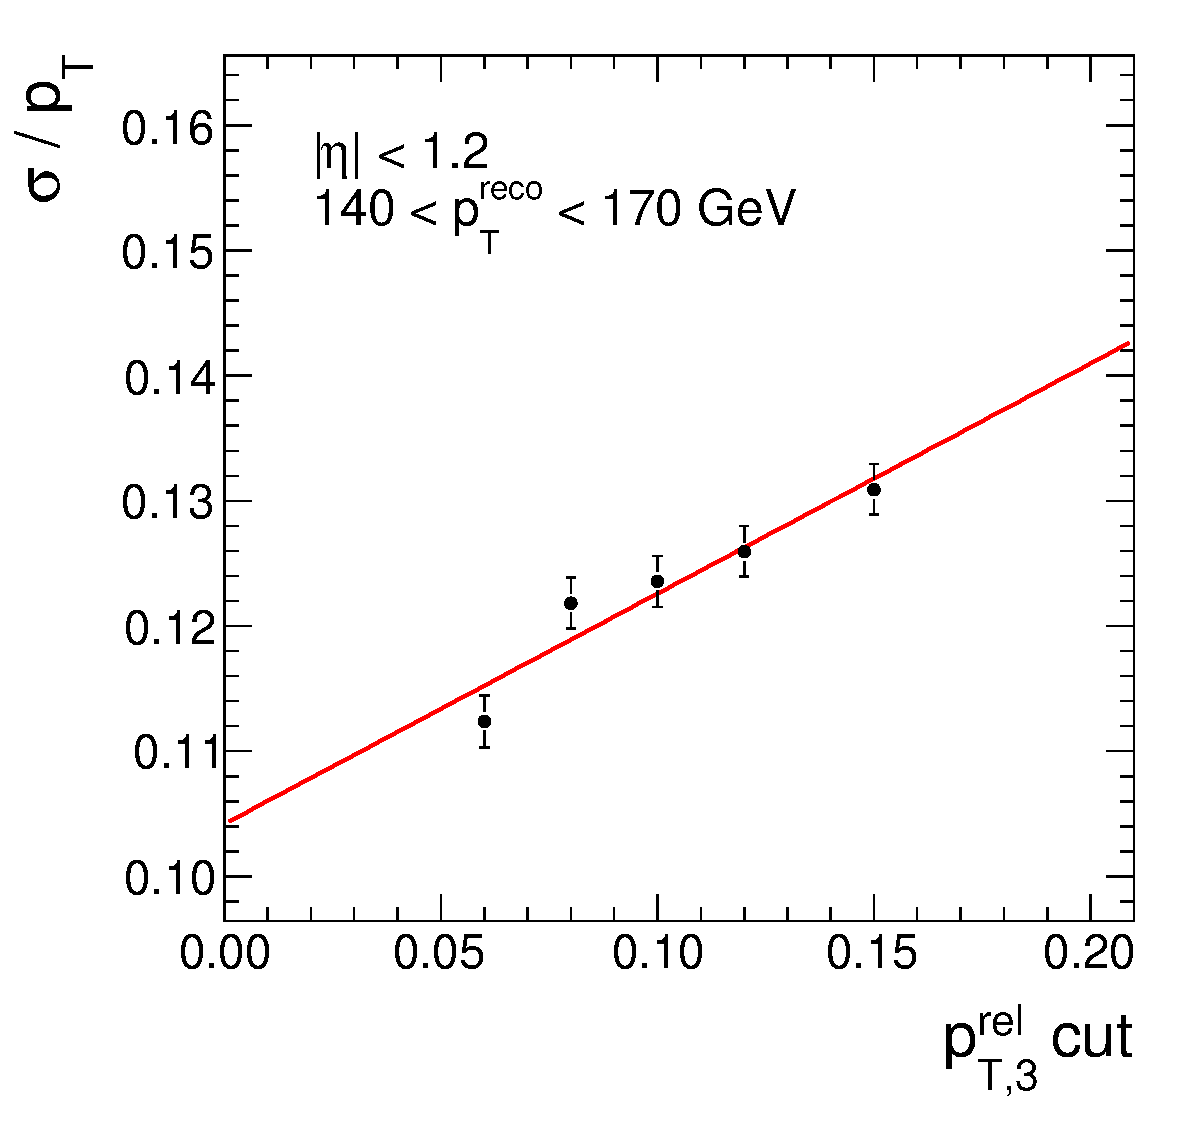
\includegraphics[width=0.3\textwidth]{figures/ResFit_Spring10QCDFlat_CB_Eta0_ExtrapolatedPar0_PtBin1} &
    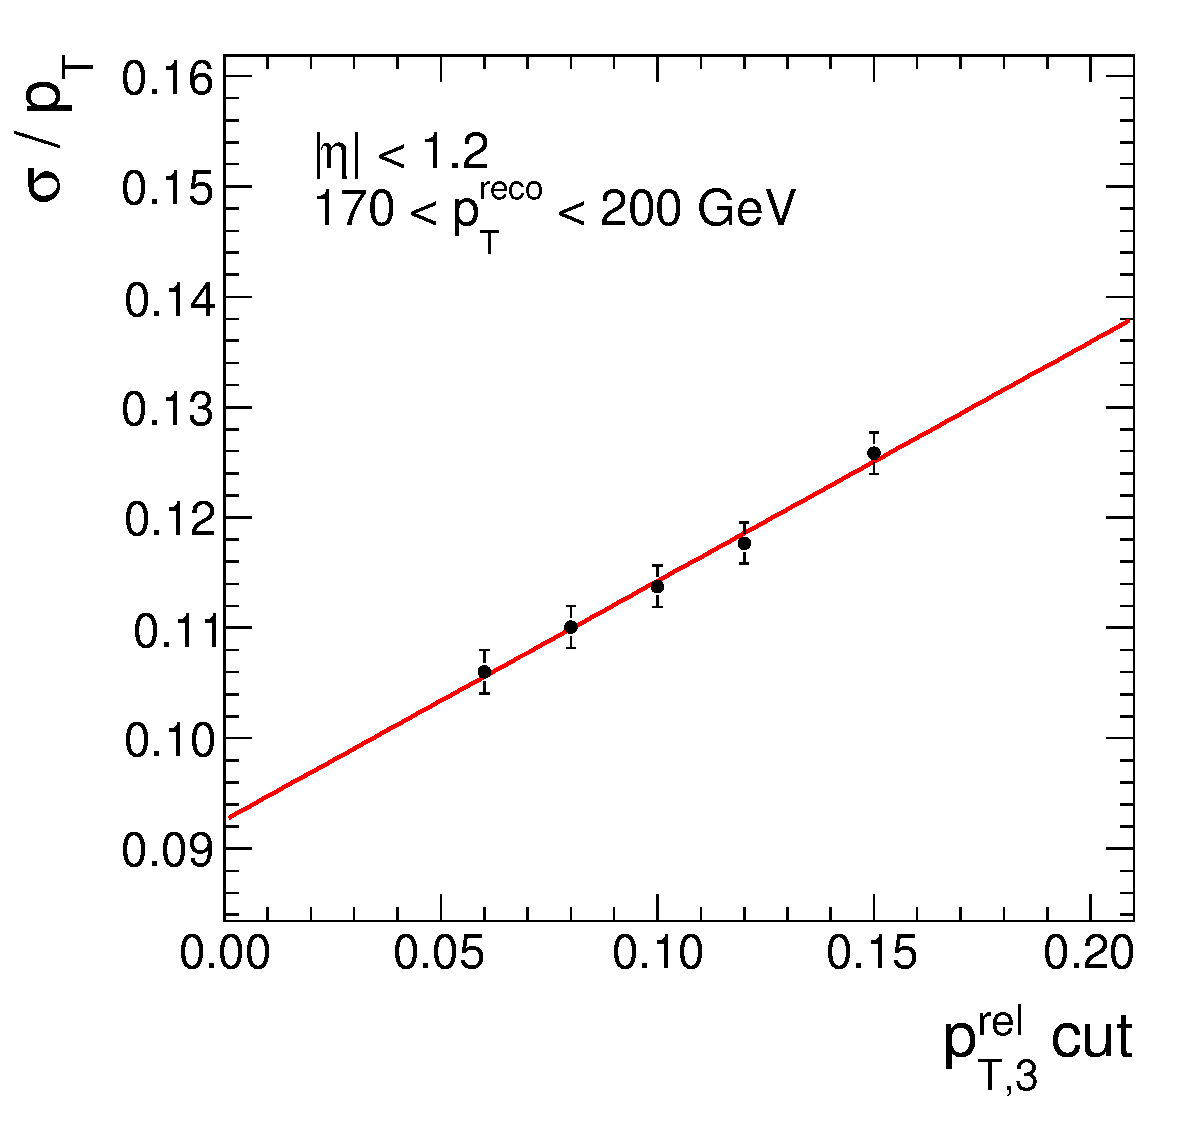
\includegraphics[width=0.3\textwidth]{figures/ResFit_Spring10QCDFlat_CB_Eta0_ExtrapolatedPar0_PtBin2} \\

    \includegraphics[width=0.3\textwidth]{figures/ResFit_Spring10QCDFlat_CB_Eta0_ExtrapolatedPar0_PtBin3} &
    \includegraphics[width=0.3\textwidth]{figures/ResFit_Spring10QCDFlat_CB_Eta0_ExtrapolatedPar0_PtBin4} &
    \includegraphics[width=0.3\textwidth]{figures/ResFit_Spring10QCDFlat_CB_Eta0_ExtrapolatedPar0_PtBin5} \\

    \includegraphics[width=0.3\textwidth]{figures/ResFit_Spring10QCDFlat_CB_Eta0_ExtrapolatedPar0_PtBin6} &
    \includegraphics[width=0.3\textwidth]{figures/ResFit_Spring10QCDFlat_CB_Eta0_ExtrapolatedPar0_PtBin7} &
    \includegraphics[width=0.3\textwidth]{figures/ResFit_Spring10QCDFlat_CB_Eta0_ExtrapolatedPar0_PtBin8} \\

    \includegraphics[width=0.3\textwidth]{figures/ResFit_Spring10QCDFlat_CB_Eta0_ExtrapolatedPar0_PtBin9} &
    \includegraphics[width=0.3\textwidth]{figures/ResFit_Spring10QCDFlat_CB_Eta0_ExtrapolatedPar0_PtBin10} & \\
  \end{tabular}
\caption{}
\label{fig:ResFit:App:CB:ExtrapolatedPar0}
\end{figure}

\begin{figure}[ht]
  \centering
  \begin{tabular}{ccc}
    \includegraphics[width=0.3\textwidth]{figures/ResFit_Spring10QCDFlat_CB_Eta0_ExtrapolatedPar1_PtBin0} &
    \includegraphics[width=0.3\textwidth]{figures/ResFit_Spring10QCDFlat_CB_Eta0_ExtrapolatedPar1_PtBin1} &
    \includegraphics[width=0.3\textwidth]{figures/ResFit_Spring10QCDFlat_CB_Eta0_ExtrapolatedPar1_PtBin2} \\

    \includegraphics[width=0.3\textwidth]{figures/ResFit_Spring10QCDFlat_CB_Eta0_ExtrapolatedPar1_PtBin3} &
    \includegraphics[width=0.3\textwidth]{figures/ResFit_Spring10QCDFlat_CB_Eta0_ExtrapolatedPar1_PtBin4} &
    \includegraphics[width=0.3\textwidth]{figures/ResFit_Spring10QCDFlat_CB_Eta0_ExtrapolatedPar1_PtBin5} \\

    \includegraphics[width=0.3\textwidth]{figures/ResFit_Spring10QCDFlat_CB_Eta0_ExtrapolatedPar1_PtBin6} &
    \includegraphics[width=0.3\textwidth]{figures/ResFit_Spring10QCDFlat_CB_Eta0_ExtrapolatedPar1_PtBin7} &
    \includegraphics[width=0.3\textwidth]{figures/ResFit_Spring10QCDFlat_CB_Eta0_ExtrapolatedPar1_PtBin8} \\

    \includegraphics[width=0.3\textwidth]{figures/ResFit_Spring10QCDFlat_CB_Eta0_ExtrapolatedPar1_PtBin9} &
    \includegraphics[width=0.3\textwidth]{figures/ResFit_Spring10QCDFlat_CB_Eta0_ExtrapolatedPar1_PtBin10} & \\
  \end{tabular}
\caption{}
\label{fig:ResFit:App:CB:ExtrapolatedPar1}
\end{figure}

\begin{figure}[ht]
  \centering
  \begin{tabular}{ccc}
    \includegraphics[width=0.3\textwidth]{figures/ResFit_Spring10QCDFlat_CB_Eta0_ExtrapolatedPar2_PtBin0} &
    \includegraphics[width=0.3\textwidth]{figures/ResFit_Spring10QCDFlat_CB_Eta0_ExtrapolatedPar2_PtBin1} &
    \includegraphics[width=0.3\textwidth]{figures/ResFit_Spring10QCDFlat_CB_Eta0_ExtrapolatedPar2_PtBin2} \\

    \includegraphics[width=0.3\textwidth]{figures/ResFit_Spring10QCDFlat_CB_Eta0_ExtrapolatedPar2_PtBin3} &
    \includegraphics[width=0.3\textwidth]{figures/ResFit_Spring10QCDFlat_CB_Eta0_ExtrapolatedPar2_PtBin4} &
    \includegraphics[width=0.3\textwidth]{figures/ResFit_Spring10QCDFlat_CB_Eta0_ExtrapolatedPar2_PtBin5} \\

    \includegraphics[width=0.3\textwidth]{figures/ResFit_Spring10QCDFlat_CB_Eta0_ExtrapolatedPar2_PtBin6} &
    \includegraphics[width=0.3\textwidth]{figures/ResFit_Spring10QCDFlat_CB_Eta0_ExtrapolatedPar2_PtBin7} &
    \includegraphics[width=0.3\textwidth]{figures/ResFit_Spring10QCDFlat_CB_Eta0_ExtrapolatedPar2_PtBin8} \\

    \includegraphics[width=0.3\textwidth]{figures/ResFit_Spring10QCDFlat_CB_Eta0_ExtrapolatedPar2_PtBin9} &
    \includegraphics[width=0.3\textwidth]{figures/ResFit_Spring10QCDFlat_CB_Eta0_ExtrapolatedPar2_PtBin10} & \\
  \end{tabular}
\caption{}
\label{fig:ResFit:App:CB:ExtrapolatedPar2}
\end{figure}


% ----- Crystal Ball Eta0 MCClosure -----
\begin{figure}[ht]
  \centering
  \begin{tabular}{ccc}
    \includegraphics[width=0.3\textwidth]{figures/ResFit_Spring10QCDFlat_CB_Eta0_MCClosure_PtBin0} &
    \includegraphics[width=0.3\textwidth]{figures/ResFit_Spring10QCDFlat_CB_Eta0_MCClosure_PtBin1} &
    \includegraphics[width=0.3\textwidth]{figures/ResFit_Spring10QCDFlat_CB_Eta0_MCClosure_PtBin2} \\

    \includegraphics[width=0.3\textwidth]{figures/ResFit_Spring10QCDFlat_CB_Eta0_MCClosure_PtBin3} &
    \includegraphics[width=0.3\textwidth]{figures/ResFit_Spring10QCDFlat_CB_Eta0_MCClosure_PtBin4} &
    \includegraphics[width=0.3\textwidth]{figures/ResFit_Spring10QCDFlat_CB_Eta0_MCClosure_PtBin5} \\

    \includegraphics[width=0.3\textwidth]{figures/ResFit_Spring10QCDFlat_CB_Eta0_MCClosure_PtBin6} &
    \includegraphics[width=0.3\textwidth]{figures/ResFit_Spring10QCDFlat_CB_Eta0_MCClosure_PtBin7} &
    \includegraphics[width=0.3\textwidth]{figures/ResFit_Spring10QCDFlat_CB_Eta0_MCClosure_PtBin8} \\

    \includegraphics[width=0.3\textwidth]{figures/ResFit_Spring10QCDFlat_CB_Eta0_MCClosure_PtBin9} &
    \includegraphics[width=0.3\textwidth]{figures/ResFit_Spring10QCDFlat_CB_Eta0_MCClosure_PtBin10} & \\
  \end{tabular}
\caption{Closure \mbox{$|\eta|<1.2$}.}
\label{fig:ResFit:App:CB:MCClosure}
\end{figure}

\clearpage